\documentclass[capchap,capsec,sumarioincompleto,a4paper,12pt,plainheader,normaltoc]{utfprtex}%

%\usepackage{utfprtexPropostaTCC} 	% mt: usar quando for a proposta. Nesse caso, elimine as quinquilharias também (rosto, banca, ata, etc.)
\usepackage{utfprtexTCC}	
\usepackage[T1]{fontenc}% pacote para acentuação Português
\usepackage[brazil]{babel} % pacote portugues brasileiro
\usepackage[utf8]{inputenc}
\usepackage{amsmath,amsfonts,amssymb} % pacote matematico
\usepackage{graphicx}
\usepackage{float}
\usepackage{circuitikz}
\usepackage{listings}
\usepackage{tikz}
\usepackage{psfrag,stmaryrd,array,comment,pxfonts,subfig,textcomp}
\usepackage{amsmath}
\usepackage{geometry}
\usepackage[breaklinks=true,linktocpage=true,pdfauthor={Jefferson Willian França Góes},pdftitle={Trabalho de Conclusão de Curso 2},pdfsubject={Trabalho de Conclusão de Curso 2}]{hyperref}
\usepackage[alf,abnt-emphasize=bf,abnt-etal-text=it,bibjustif,abnt-etal-cite=2,abnt-etal-list=0,abnt-full-initials=yes]{abntcite}
\usepackage{nomencl}
\usepackage{graphicx,psfrag,stmaryrd,array,psfrag}
\usepackage{multirow}
\usepackage{xcolor}
\usepackage{listings}
\usepackage{nomencl}
\usepackage{chngcntr}
\definecolor{mGreen}{rgb}{0,0.6,0}
\definecolor{mGray}{rgb}{0.5,0.5,0.5}
\definecolor{mPurple}{rgb}{0.58,0,0.82}
\definecolor{backgroundColour}{rgb}{0.95,0.95,0.92}

\definecolor{deepblue}{rgb}{0,0,0.5}
\definecolor{deepred}{rgb}{0.6,0,0}
\definecolor{deepgreen}{rgb}{0,0.5,0}

\lstdefinestyle{CStyle}{
	backgroundcolor=\color{backgroundColour},   
	commentstyle=\color{mGreen},
	keywordstyle=\color{magenta},
	numberstyle=\tiny\color{mGray},
	stringstyle=\color{mPurple},
	basicstyle=\footnotesize,
	breakatwhitespace=false,         
	breaklines=true,                                  
	keepspaces=true,                 
	numbers=left,                    
	numbersep=5pt,                  
	showspaces=false,                
	showstringspaces=false,
	showtabs=false,                  
	tabsize=2,
	language=C
}

\lstdefinestyle{Python}{
	language=Python,
	otherkeywords={self},             % Add keywords here
	keywordstyle=\color{deepblue},
	emphstyle=\color{deepred},    % Custom highlighting style
	stringstyle=\color{deepgreen},
	frame=tb,                         % Any extra options here
	showstringspaces=false            % 
}

\usepackage{Refs/des}
\usetikzlibrary{decorations.pathreplacing, arrows, positioning, calc, chains,fit,shapes}
\geometry{
 a4paper,
 left=30mm,
 top=30mm,
 bottom=20mm,
right=20mm
 }
\setlength{\parindent}{1.5cm}

%\hyphenation{}

\fazlistasiglas % Parâmetro opcional é o título da lista.

\newcommand*{\captionsource}[2]{%
  \caption[{#1}]{%
    #1%
    \\\hspace{\linewidth}%
    \textbf{Fonte:} #2%
  }%
}


\renewcommand{\lstlistingname}{Código}% Listing -> Algorithm
\renewcommand{\lstlistlistingname}{Lista de Códigos}%


\renewcommand{\floatpagefraction}{0.90}
\renewcommand{\topfraction}{0.95}
\renewcommand{\bottomfraction}{0.95}
\renewcommand{\textfraction}{0.05}
\setlength{\intextsep}{5pt}
\setlength{\textfloatsep}{5pt}
\setlength{\floatsep}{5pt}

\pdfstringdefDisableCommands{\edef\uppercase{}}

\autorA{Jefferson Willian França Góes}
\titulo{Aperfeiçoamento de um Sistema de reconhecimento de padrões do alfabeto de libras utilizando luva sensora}

\orientador{Prof. Dr. Fábio Luiz Bertotti}
\coorientador{Prof. Dr. Dalcimar Casanova}

\palavraschave{Redes Neurais. Microcontroladores. Processamento de sinais. LIBRAS} % Palavras chave
\keywords{Neural Network. Microcontroller. Signal Processing. LIBRAS} % Palavras chave em inglês

\bancaA{Prof. Dr. Ricardo Bernardi}
\bancaB{Prof Dra. Kathya Linares}

\local{Pato Branco}

\data{2019} 

%%%%%%%%% Fim das definições iniciais %%%%%%%%%

\begin{document} 
    \counterwithout{lstlisting}{chapter}
\capa 
\folhaderosto

	\tikz[remember picture,overlay] \node[opacity=1,inner sep=0pt] at (current page.center){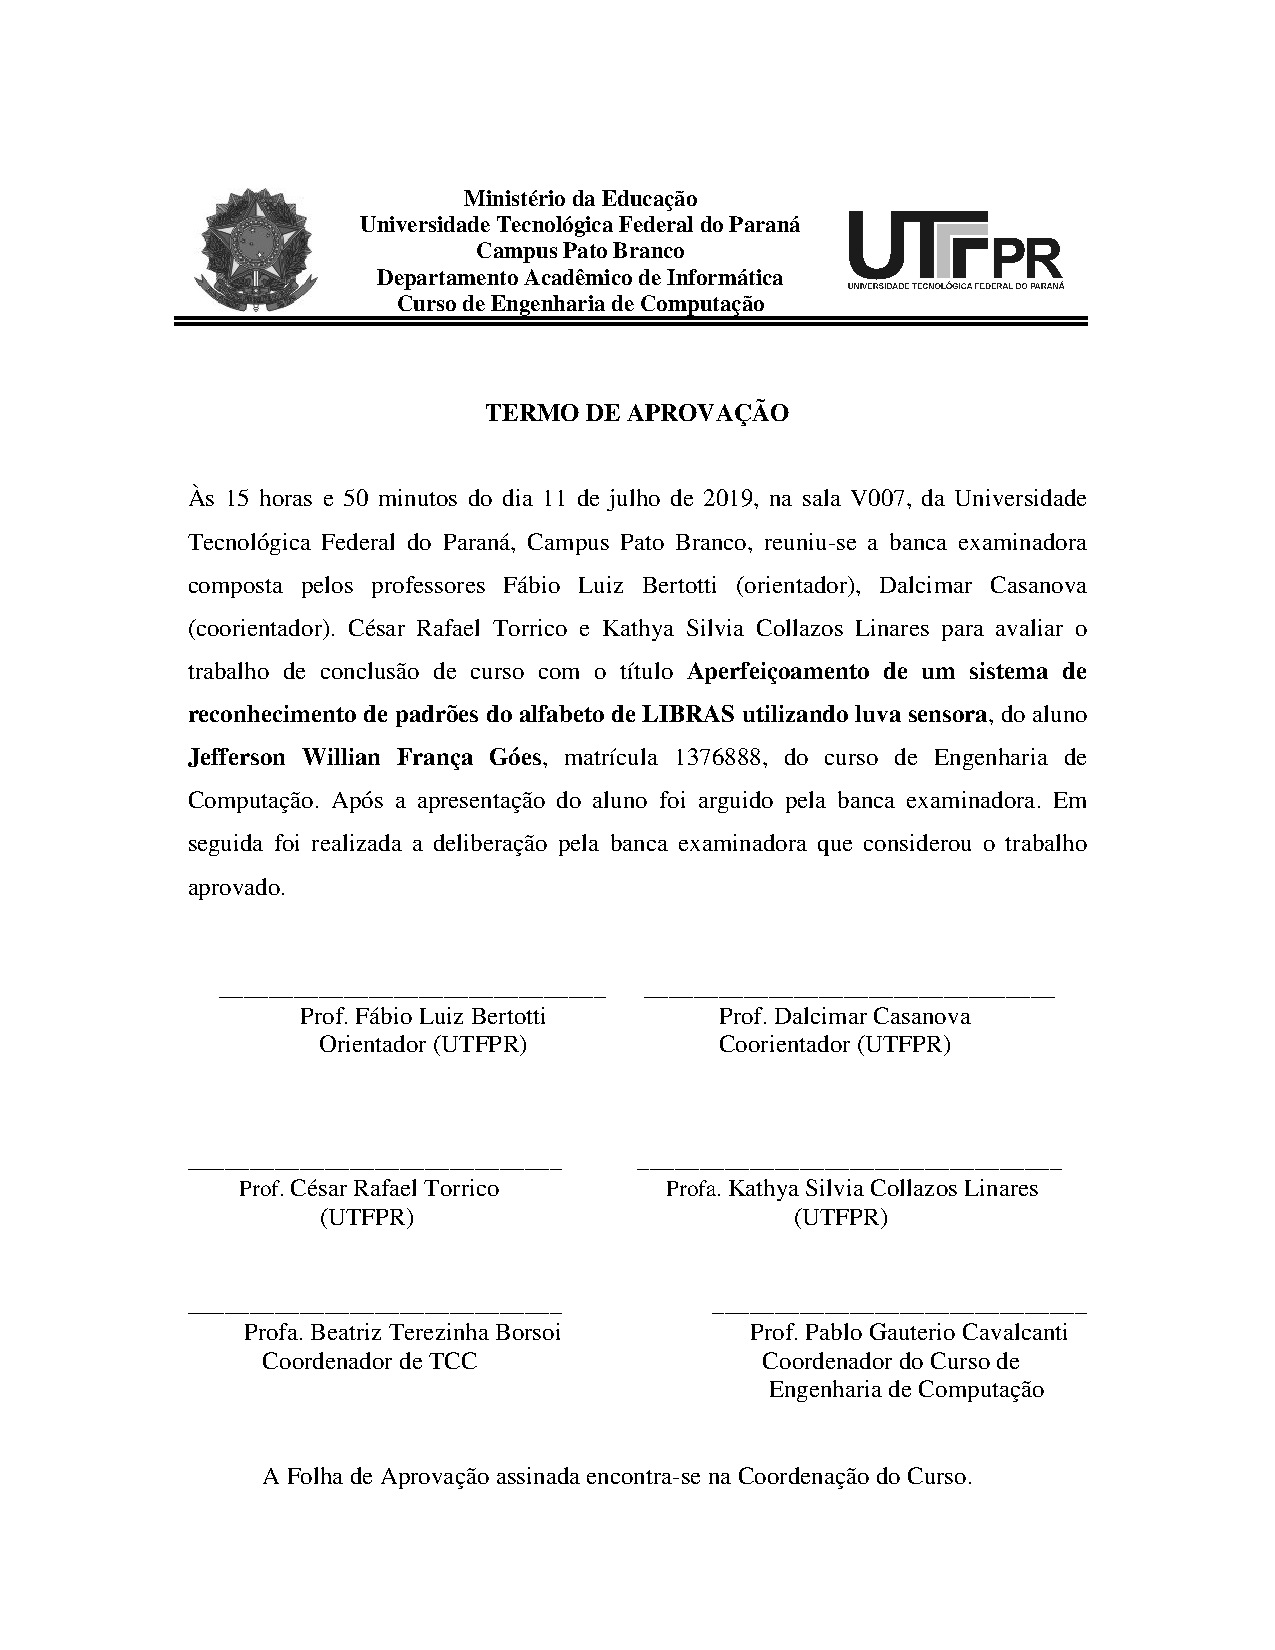
\includegraphics[width=\paperwidth,height=\paperheight]{imagens/termodeaprovacao.pdf}};
	\clearpage

% EPIGRAFE (opcional).
\begin{Epigrafe}{Alan Turing} % Parametro obrigatorio entre {} é o autor da epigrafe.
	Um computador pode ser chamado de inteligente se ele pode enganar uma pessoa a pensar que é um ser humano.
\end{Epigrafe}


%% AGRADECIMENTOS
\begin{Agradecimentos}
Primeiramente agradeço ao meu orientador pela sugestão de um trabalho que já foi feito, dando continuidade aos trabalhos feitos por outros acadêmicos. Também agradeço ao meu coorientador pelo suporte dado em relação as redes neurais e como fazer tudo isso funcionar. Agradecendo também a minha namorada pelas correções fornecidas no trabalho e estar ao meu lado nessa jornada que também se estende à minha família e amigos que me aguentaram e me ajudaram nesta fase difícil da faculdade. E por último mas não menos importante um agradecimento aos professores em geral que me fizeram evoluir e descobrir mais sobre eu mesmo para superar todos os desafios.
\end{Agradecimentos}

% RESUMO:
\begin{Resumo}
%\hspace*{-1.53cm}GÓES, Jefferson W. F. APERFEIÇOAMENTO DE UM SISTEMA DE RECONHECIMENTO DE PADRÕES DO ALFABETO DE LIBRAS UTILIZANDO LUVA SENSORA. 2019. 46f. Monografia (Trabalho de Conclusão de Curso 2) - Curso de Engenharia de Computação, Universidade Tecnológica Federal do Paraná, Câmpus Pato Branco. Pato Branco, 2019.\par\quad\par

\hspace*{-1.53cm}Linguagem Brasileira de Sinais (LIBRAS) é uma língua gestual-visual amplamente utilizada por surdos no Brasil. No ensino de LIBRAS, a interação com o objeto de ensino pode potencializar o aprendizado. A partir dessa premissa, acredita-se que um sistema de detecção do alfabeto de LIBRAS pode contribuir no processo de aprendizagem, assim como na tradução da linguagem em elementos textuais. Desta forma, este trabalho apresenta o 
aperfeiçoamento de um sistema para reconhecimento de padrões do alfabeto de LIBRAS utilizando uma luva sensora previamente concebida. Como resultado, obteve-se um sistema que utiliza redes neurais capaz de reconhecer todas as letras do alfabeto, com um percentual de acerto de 84%.
\end{Resumo}

% ABSTRACT
\begin{Abstract}
%\hspace*{-1.53cm}GÓES, Jefferson. IMPROVEMENT OF A PATTERN RECOGNITION SYSTEM FOR LIBRAS ALPHABET USING A SENSING GLOVE. 2019. 68f. Monografia (Trabalho de Conclusão de Curso 2) - Curso de Engenharia de Computação, Universidade Tecnológica Federal do Paraná, Câmpus Pato Branco. Pato Branco, 2019. \par\quad\par


\hspace*{-1.53cm}The Brazilian Sign Language (LIBRAS) it's a gestural-visual language used by deaf people in Brazil. In the teaching of LIBRAS, an interaction with the object of teaching can potentiate learning. From this premise, it is believed that a system of detection of the alphabet of LIBRAS can contribute in the learning process, as well as in the translation of the language into textual elements. Thus, this work presents the improvement of a system for recognizing patterns of the alphabet of LIBRAS using a previously conceived sensor glove. As a result, we obtained a system that uses neural networks capable of recognizing all the letters of the alphabet, with a correct percentage of 84%.
\end{Abstract}


\listadefiguras
%\listofquadros
\listadetabelas

\newpage
\section*{\textbf{Lista de Siglas}}
\vspace{10mm}

\begin{itemize}
	\item[ADC] \hspace{30mm} Conversor Analógico Digital
	\item[fem] \hspace{30mm} Força Eletromotriz
	\item[MEMS] \hspace{30mm} Sistemas microeletromecânicos
	\item[MLP] \hspace{30mm} Perceptron Multicamada
\end{itemize}


\sumario

\chapter{Considerações Iniciais} \label{consideracoes_iniciais}
A linguagem de sinais (LS), é uma idioma não verbal, altamente desenvolvida e organizada, na qual indivíduo usa expressões faciais 
e gestos com as mãos para se expressar. Nem todas as pessoas conseguem entender e compreender uma linguagem baseada em sinais, os 
que compreendem, geralmente, são membros da família ou membros da comunidade surda \cite{smartglovecommunication}.

Para \citeonline{Comunicacao}, a Língua Brasileira de Sinais (LIBRAS) é considerado como um idioma que possui uma estrutura 
gramatical própria, contendo particularidades idiomáticas e variações regionais, as quais assemelham-se ao sotaque ou gírias. 
Contudo é importante ressaltar a diferença entre LIBRAS e o alfabeto manual, o qual é um recurso para os falantes da língua de 
sinais que auxilia na representação de siglas, lugares ou algum vocabulário para o qual não existe sinal definido \cite{LIBRAS?}.

Considerando as dificuldades de interação entre as pessoas que falam e os surdos, o protótipo desenvolvido como resultado deste 
trabalho visa prover uma forma de interação mais efetiva entre essas pessoas utilizando o alfabeto de sinais.

O propósito deste trabalho se deriva do projeto já implementado, o qual tinha por objetivo a elaboração de uma luva com sensores 
indutivos para detecção do alfabeto manual de LIBRAS. O sucesso em detectar letras as quais não possuem movimento serão levados em 
conta na implementação de um sensor inercial \cite[p. 95]{RUANI}.

A detecção do alfabeto manual somente com sensores indutivos, dispostos em uma luva sensora construído por \citeonline{RUANI}, 
possui limitações quando há padrões com movimento, sendo necessária a inclusão de um sensor inercial na luva para o reconhecimento 
de padrões com movimento.

Levando em consideração o que já foi desenvolvido, ao introduzir um sensor do tipo inercial ao sistema, a captura de dados é sensível ao tempo, e os dados devem ser processados. O microcontrolador atual (MSP430) não suportaria tal carga, sendo necessário o \textit{upgrade} para um ARM Cortex-M3. 
Considerando que serão classificados há uma necessidade de modificar a rede neural já implementada.

\section{Objetivos}
\subsection{Objetivo Geral}
	Aperfeiçoar um sistema para detecção de padrões do alfabeto de LIBRAS por meio de luva sensora, adicionando um sensor 
inercial e promovendo melhorias de \textit{hardware} necessárias para suportar o processamento dos dados do sensor inercial.
\subsection{Objetivos Específicos}
\begin{itemize}

	\item Portar um código existente para o microcontrolador STM32F103C8T6;

	\item Implementar o sensor inercial MPU-6050;

	\item Coletar dados para treinamento e validação de um algoritmo de classificação;

	\item Utilizar algoritmos de aprendizado em Python para realizar treinamento e simulações;

	\item Implementar o algoritmo de classificação no microcontrolador;

	\item Desenvolver uma interface para visualização dos resultados da classificação;

	\item Testar e validar o sistema a partir de outros usuários.

\end{itemize}

%\section{Organização do trabalho}
%%Referencial Teórico
\chapter{Referencial Teórico}
\section{Libras}

A Língua Brasileira de Sinais (LIBRAS) é um idioma que possui uma estrutura gramatical própria, contendo particularidades 
idiomáticas e regionalismos, que se assemelham ao sotaque ou as gírias da língua portuguesa. Cada país fala uma língua diferente, 
nos Estados Unidos, por exemplo, é utilizada a \textit{American Sign Language} (ASL), com seu vocabulário derivado da Língua 
Francesa de Sinais há 180 anos, e LIBRAS, também é derivada da Língua Francesa de Sinais. Embora a Inglaterra e Estados Unidos tenham inglês como idioma principal, as 
línguas de sinais são completamente diferentes. Isto também serve para o português e LIBRAS, onde LIBRAS não é o português 
sinalizado.\cite{Comunicacao}.

Para \citeonline{Zieren2006b}, em linguagens de sinais em geral, a informação é gerada por combinação dos seguintes fatores: 
configuração de mão; posicionamento da mão ou ponto de articulação; movimento; orientação (direção do sinal); e expressão facial e 
corporal.
Alguns sinais podem ser distinguidos pela configuração de mão somente, e em outros casos é a combinação de todos os fatores que 
devem ser executados evitando uma interpretação ambígua.

Em alguns casos, não existem sinais que expressem siglas, nomes, ações ou gírias. Então é desenvolvido de um alfabeto manual 
(vide Figura \ref{fig:alfabeto}) que é constituído de configuração de mão que representa uma letra e, em alguns casos, um 
movimento. Através da datilologia ou soletração digital, este alfabeto é utilizado para expressar essas palavras para as quais não 
existe um sinal equivalente  \cite{PorUmaGramatica}.


\begin{figure}[H]
	\centering
	\vspace{4mm}
	\caption{Alfabeto manual de LIBRAS}
	\label{fig:alfabeto}
	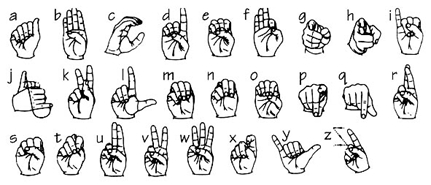
\includegraphics[scale =0.5]{imagens/Alfabeto_Libras.jpeg}
	\caption*{Fonte: \citeonline{Comunicacao}.}
\end{figure}


Como a Figura \ref{fig:CERTO} apresenta, a palavra "certo" que em datilologia exige cinco gestos para definir o  seu significado, 
enquanto utilizando o sinal existente, pode ser definida apenas com um gesto.
\begin{figure}[H]
	\vspace{4mm}
	\centering
	\caption{Comparação entre datilologia e sinal pronto da palavra certo}
	\label{fig:CERTO}
	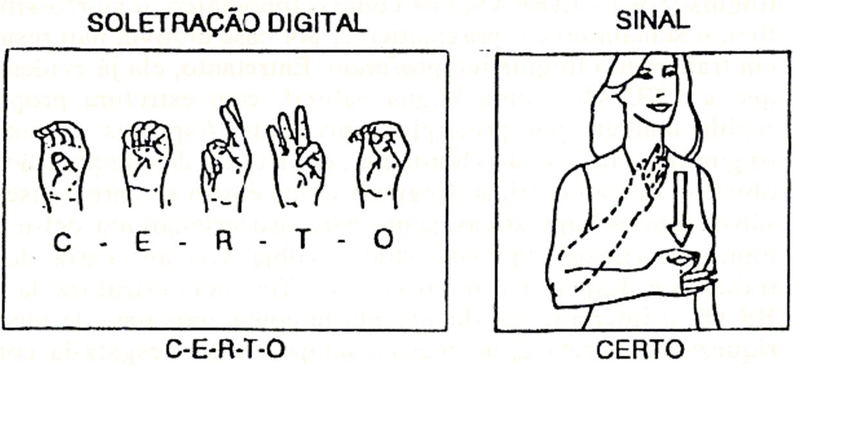
\includegraphics[scale=0.4, trim={0 1cm 2cm 0}, clip]{imagens/Certo}
	\caption*{Fonte: \citeonline[p. 22]{PorUmaGramatica}.}
\end{figure}

Existem ainda, muitas limitações no processo de comunicação, entre surdos e ouvintes em ambientes como
trabalho, escolas, universidades e no próprio ambiente familiar de surdos, provocando um distanciamento
\cite{jogoslibras}, que podem ser minimizadas, gradativamente, pelo
uso de objetos de aprendizagem \cite{ferramentas}.


Conforme \citeonline{martinsEmatos}, as tecnologias podem facilitar a inserção comunicativa dos surdos, assim como para os ouvintes, com o uso
frequente, por exemplo, das redes sociais, que apesar de primar pelo lazer, possibilitam um maior contato com o
português, uso de dicionários on-line e os objetos de aprendizagem (hipermídias, softwares, jogos etc), permitindo
aos surdos, o contato com materiais mais interessantes e atrativos.




\section{Luvas Sensoras}
Segundo \citeonline{baseadoruani} mapeamento de mão é a tecnologia  mais popular para entrada de dados na Realidade Virtual  (VR). As entradas baseadas em luva permitem que o usuário aplique a sua coordenação e habilidade para as atividades de VR. Os tipos de luvas abordados são as luvas mais expressivas no mercado, e a luva indutiva que é a luva utilizada neste trabalho.


\subsection{Luva com sensores de fibra ótica}
As luvas de dados baseadas em sensores de fibra ótica usam um LED emissor de infravermelho como fonte, com o sinal sendo 
conduzido por um tubo flexível de fibra. Então, uma fotocélula é colocado no outro lado e mede a intensidade do sinal enviado via 
fibra \cite{baseadoruani}.
		
A luva de dados 5DT Data Glove 16 da empresa Five Dimention Technologies, demonstrada na Figura \ref{fig:5DT}, com 15 sensores de fibra ótica, 2 em cada dedo e 
1 sensor na junta do dedo. E um último, um sensor inercial para determinar os movimentos circulares com a luva. Contém também 
Conversor A/D (Analógico para digital) de até 12 bits para cada sensor. Da luva inteira (14 sensores) podem ser obtidas até 100 
amostras por segundo \cite{FiveD}.

\begin{figure}[H]
	\vspace{4mm}
    \centering
    \caption{Luva com sensores de fibra ótica da Five Dimension Tecnologies}
    \label{fig:5DT}
    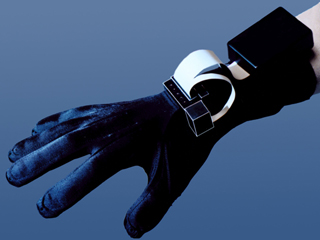
\includegraphics[scale=0.6]{imagens/5DT_Glove.jpeg}    
    \caption*{Fonte: \citeonline{FiveD}.}
\end{figure}
	

	\subsection{Luva com sensores de flexão}	
Os sensores de flexão  utilizam um material que varia a resistência de acordo com o grau da dobra realizada, utilizando uma 
escala de 0 a 90 graus. Em luvas que utilizam esse tipo de sensor são colocados cinco sensores, um para cada dedo. Quando os dedos 
são flexionados, a resistência do sensor varia resultando em uma tensão equivalente ao grau de flexão de cada dedo. 
\cite{baseadoruani}.
	
A empresa CyberGlove Systems produz uma série de luvas para o desenvolvimento de animações e captura de movimentos, entre elas, a CyberGlove III que pode ser vista na Figura \ref{fig:CyberGlove}, a qual faz uso de 22 sensores de flexão com resolução menor do que um grau. Também dispõe de interface 
Wi-Fi e conexão para cartão USB \cite{cGlove}.
	
	
	\begin{figure}[H]
		\vspace{4mm}
		\centering
		\caption{Luva de dados CyberGlove III da Cyber Glove Systems LLC}
		\label{fig:CyberGlove}
		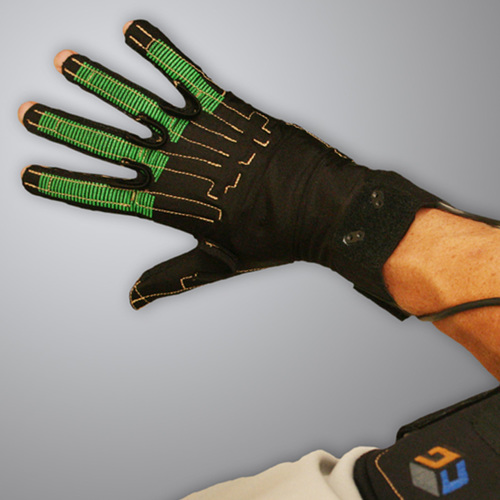
\includegraphics[scale=0.3]{imagens/CyberGlove.jpeg}		
		\caption*{Fonte: \citeonline{cGlove}.}
	\end{figure}
	
	\section{Luva com sensores inerciais}
	
Em luvas com sensores inerciais, os sensores são calibrados em um mesmo ponto onde é considerado o eixo zero, com base nessa calibragem são utilizados 2 sensores entre uma junta para medir o ângulo das duas partes do dedo em relação a junta \cite{calculojunta}.

Um exemplo deste tipo é a IGS Cobra da empresa Synertial(vide \ref{fig:Cobra}), com 16 sensores inerciais com 9 eixos de liberdade 
(acelerômetro, giroscópio e magnetômetro) \cite{synert}.
		
		
	\begin{figure}[H]
		\vspace{4mm}
		\centering
		\caption{Luva de dados IGS Cobra da Synertial}
		\label{fig:Cobra}
		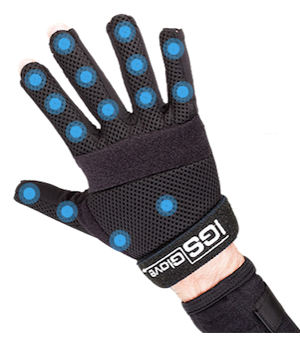
\includegraphics[scale=0.5]{imagens/Cobra.png}		
		\caption*{Fonte: \citeonline{synert}}
	\end{figure}

		
		
\subsection{Luva com sensores indutivos}
Uma luva indutiva ou luva com sensores indutivos utiliza um sensor de rastreamento magnético, onde uma fonte irradia um campo magnético e um pequeno sensor retorna a posição e orientação em relação a fonte magnética. O princípio de  funcionamento será abordado na seção \ref{sec:indutivo}.
\section{Trabalho Previamente Desenvolvido}
O trabalho elaborado por \citeonline{RUANI} tinha como objetivo geral: Desenvolver um dispositivo do tipo luva sensora capaz de 
reconhecer configurações de mão, correspondente ao alfabeto manual de LIBRAS, e realizar a tradução destas para o seu significado 
na Língua Portuguesa, apresentando o resultado na forma de texto em um \textit{display}. A luva foi desenvolvida a partir de sensores indutivos, incluindo circuito de excitação
para as bobinas, assim como circuito de leitura e sistema embarcado usando o 
microcontrolador MSP430F5529.

\subsection{Construção das bobinas}
Com base no trabalho de \citeonline{baseadoruani}, foi possível obter um método para construir uma luva com sensores indutivos 
que tem o funcionamento explicado na seção \ref{sec:indutivo}. 	
Para obter a posição dos sensores na luva foi observado diferentes sinais de LIBRAS e como eles se diferem, por exemplo U e V, 
somente o ângulo entre o dedo indicador e dedo médio pode diferenciar essas letras. Considerando todas as letras e suas posições 
de mão, foi obtido o seguinte esquema de sensores e geradores, como demonstrado na Figura \ref{fig:disposicaoSensores}.

	\begin{figure}[H]
		\vspace{4mm}
		\centering
		\caption{Mapa de sensores e geradores de sinal na luva}
		\label{fig:disposicaoSensores}
		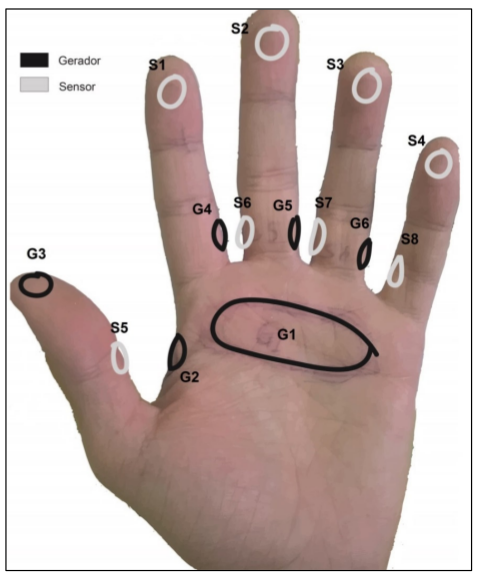
\includegraphics[scale=0.5]{imagens/SensoresMao.png}		
		\caption*{Fonte: \citeonline[p. 68]{RUANI}.}		
	\end{figure}
	
	
A espessura das bobinas foi definida para que não atrapalhasse no movimento normal da mão ao vestir a luva, tendo $14\textrm{ }mm$ de 
diâmetro. Todas as bobinas foram construídas a mão e com o mesmo número de espiras. Naturalmente que devido ao processo manual de 
fabricação há uma variação nas indutâncias. A frequência ressonante  do circuito LC foi definida em torno de $100\textrm{ }kHz$, 
projetando o 
resto dos componentes a partir disso. Uma das bobinas construídas é exibida na Figura \ref{fig:bobinas}.


	\begin{figure}[H]
		\vspace{4mm}
		\centering
		\caption{Bobina construída para luva}
		\label{fig:bobinas}
		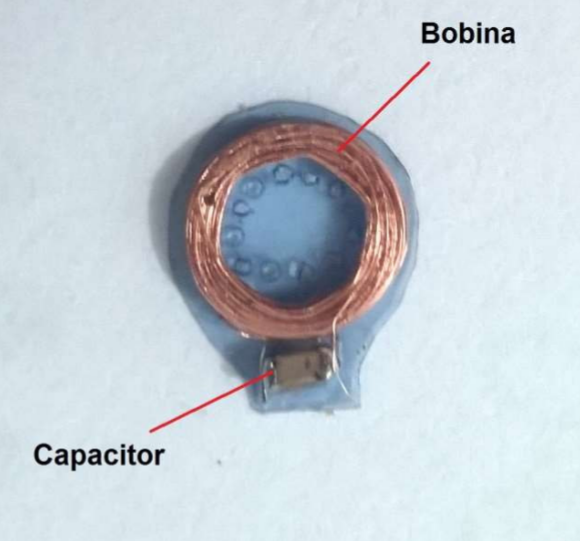
\includegraphics[scale=0.25]{imagens/SensorIndutivo.png}
		\caption*{Fonte: \citeonline[p. 71]{RUANI}.}		
	\end{figure}

 O resultado é apresentado na Figura \ref{fig:luvaRuani}, onde é mostrada a luva construída com os sensores indutivos.

	\begin{figure}[H]
		\vspace{4mm}
		\centering
		\caption{Vista frontal e lateral da luva sensora desenvolvida}
		\label{fig:luvaRuani}
		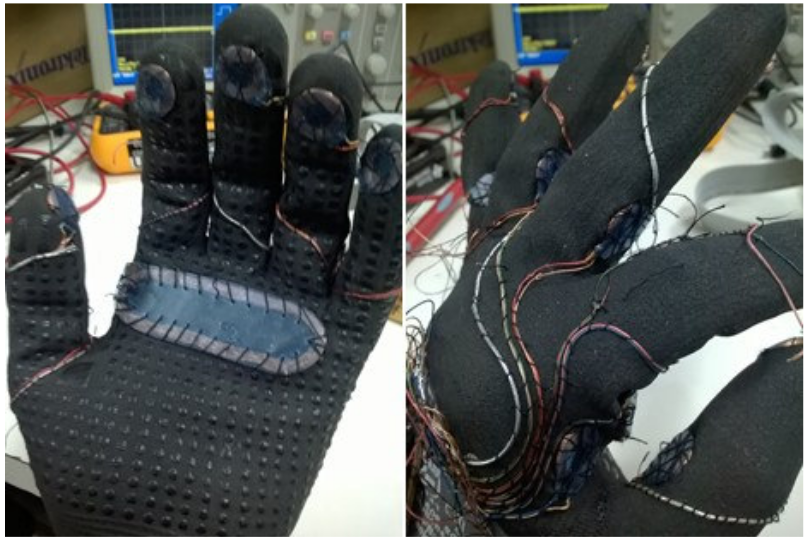
\includegraphics[scale=0.5]{imagens/luvaRuani.png}	
		\caption*{Fonte: \citeonline[p. 87]{RUANI}.}		
	\end{figure}

	

\subsection{Circuito de condicionamento de sinais}
\label{sec:placa}
Para o funcionamento do sistema como um todo, todos os sinais provenientes dos sensores indutivos devem ser tratados para a  
leitura correta no conversor analógico digital (ADC) do microcontrolador.
Na figura \ref{fig:hard} é possível ver todo o tratamento de \textit{hardware} feito para o processamento dos sinais do sensores 
indutivos.

\begin{figure}[H]
	\vspace{4mm}
  	\centering
	\caption{Diagrama de blocos do sistema desenvolvido por \citeonline[p.65]{RUANI}}		
  	\label{fig:hard}	
  	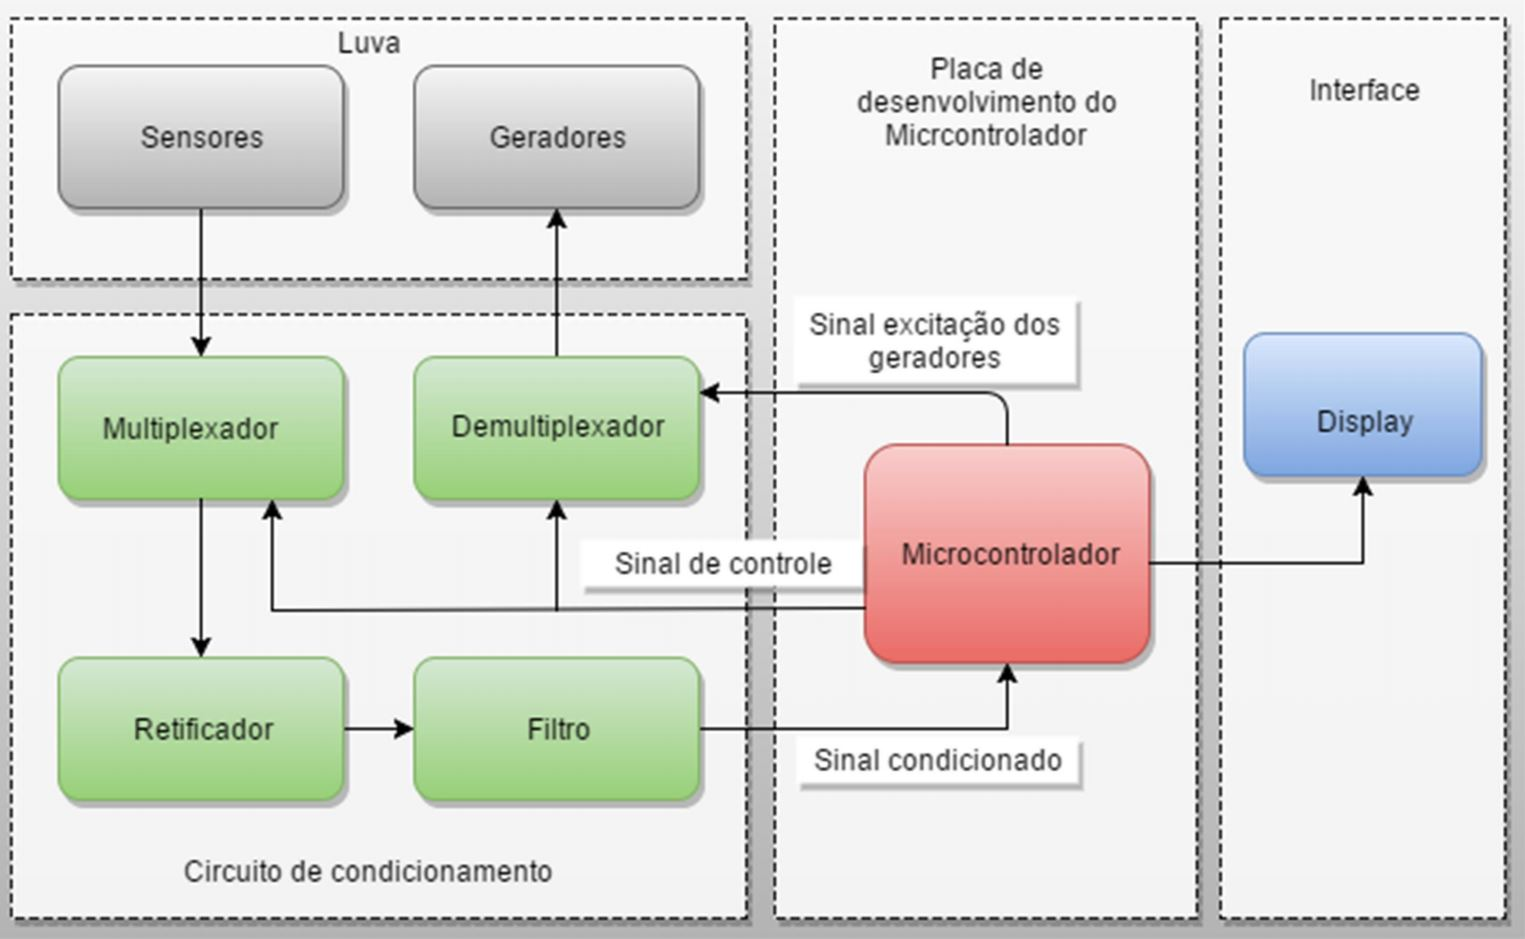
\includegraphics[scale=0.3]{imagens/desc_luva_ruani.JPG}
  	\caption*{Fonte: \citeonline[p. 65]{RUANI}.}
\end{figure}

A modelagem do circuito de aquisição e processamento dos sinais foi proposta por \citeonline{baseadoruani}, o qual 
foi adaptado para simplificar o circuito. Uma das modificações foi substituir o gerador senoidal e deixar o microcontrolador 
gerar uma onda quadrada, considerando que a mudança de forma de onda não interfere significativamente na resposta dos sensores, 
sendo que é a frequência que determina a ressonância dos geradores \cite{RUANI}.

Um circuito retificador a envoltória do sinal CC é necessário para converter um sinal CA em um sinal CC. Para que a saída represente o pico do sinal CC, 
é necessário empregar um detector de pico seguido de um filtro passa-baixas \cite{Boylestad}.

De acordo com \cite{malvinaodamassa}, um filtro permite a passagem de uma faixa de frequências enquanto rejeita outra. Filtros 
podem separar os sinais desejados dos indesejados, bloquear sinais de interferência e modificar sinais. Existem os filtros 
passivos que são constituídos de resistores, capacitores e indutores. Também existem os ativos, que são compostos de resistores, 
capacitores e amplificadores operacionais ou amp-ops.

O uso de amp-ops nos filtros ativos pode eliminar a necessidade dos volumosos indutores, que não são satisfatórios quando 
integrados aos circuítos. Em contrapartida, filtros ativos não atenuam necessariamente os sinais sobre a banda passante, como acontece 
com seus similares feitos com elementos passivos \cite{Cathey}.

Como são utilizadas várias bobinas, utiliza-se de uma técnica para não ter leituras afetadas por interferência, utilizando o 
método de divisão de tempo, onde cada bobina geradora é acionada sozinha por um período de tempo. O sinal de saída do 
multiplexador deve passar por um processo de condicionamento, primeiramente por um atenuador, para que o valor de amplitude se
fique adequado ao valor de alimentação dos amplificadores operacionais \cite{RUANI}.

Em seguida, o sinal passa por um circuito retificador, uma vez que a informação que possibilita estimar a posição das bobinas é 
o modulo da fem induzida nas bobinas dos sensores. O sinal retificado é filtrado para eliminar \textit{ripple} do sinal, e em 
seguida passa por ajustes de amplitude para ser conectado ao ADC do microcontrolador.
	

	
	
	
	
	
	
\section{Acelerômetro}		
	Um acelerômetro é um componente eletrônico que mede as forças exercidas num determinado objeto.  Essas forças podem ser de 
	dois tipos: estáticas ou dinâmicas, sendo estática a força da aceleração gravitacional (constante), e dinâmicas 
	causadas pelo movimento ou vibração provocados no acelerômetro \cite[p. 20]{LISBOA}.

	
	\subsection{Funcionamento}
	O princípio básico de um acelerômetro é a ação de aceleração de uma massa para produzir força, conforme descrito na 
	segunda lei de Newton (vide Equação \ref{eq:segunda}):

	\begin{equation}
		F = m \times a,
		\label{eq:segunda}
	\end{equation}
	onde $F$ é a força em Newtons [N], $m$ a massa em quilos [kg] e $a$ aceleração em $m/{s^2}$. Portanto, é necessário a utilização de uma massa nos acelerômetros, chamada massa inercial para medir a aceleração \cite[p. 271]{INSTRUME}. O acelerômetro pode ser modelado matematicamente como mostra na Figura \ref{fig:modeloAcc}.\\	 

		\begin{figure}[H]
		\vspace{4mm}
		\centering
		\caption{Modelo de um acelerômetro que consiste em uma massa sísmica, um elemento mola e um elemento amortecimento}		
		\label{fig:modeloAcc}	
		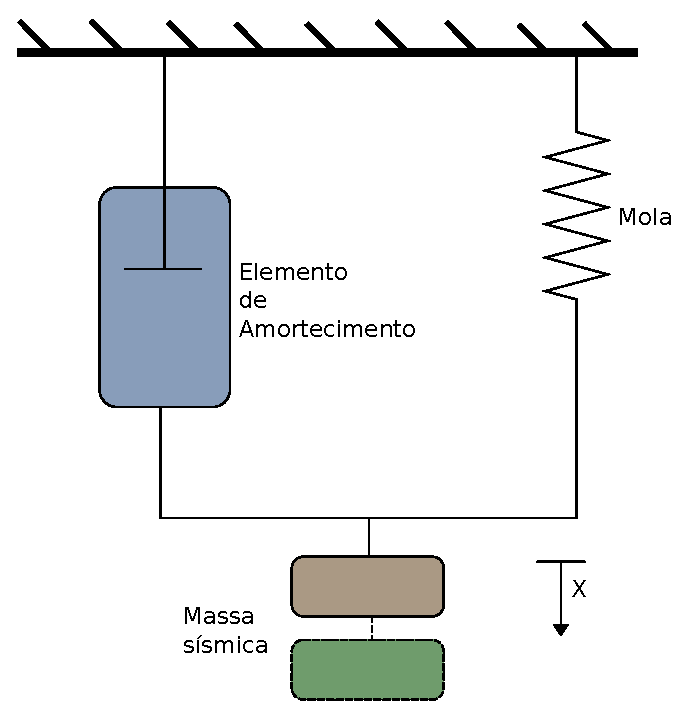
\includegraphics[scale=0.7]{imagens/massamola.eps}
		\caption*{Fonte: \citeonline[p. 271]{INSTRUME}.}
		\end{figure}
	
	Conforme a Figura \ref{fig:modeloAcc}, uma força pode ser aplicada a massa de acordo com a segunda lei de Newton, e o esquema pode ser modelado conforme \cite{INSTRUME}:
	\begin{equation}
		\frac{x(s)}{a(s)} = \frac{1}{ 	s^2 + \frac{b}{m} + s\frac{K}{m}},
		\label{eq:laplace}
	\end{equation}
	em que $s$ representa o operador de Laplace, $x$ o deslocamento da massa de sua posição de repouso, $a$ a aceleração a ser mensurada, $b$ o coeficiente de amortecimento, $m$ a massa destinada ao movimento e $K$ a constante da mola.
	
	Os acelerômetros são encontrados em diversos tamanhos e tecnologias, entre eles os piezoelétricos, piezorresistivos e capacitivos. Para reduzir o tamanho do dispositivo,são aplicadas técnicas da área de microeletrônica, resultando em um dispositivo classificado como sistema
	microeletromecânico ou MEMS (Micro-Electro-Mechanical System). \cite{INSTRUME}.

	\subsection{Eixos de rotação}
Conforme \citeonline{NASA} uma aeronave em pleno voo irá rotacionar em torno do seu centro de gravidade, que é o ponto de onde se localiza a massa média da aeronave. É possível definir um sistema de coordenadas tridimensional baseado no centro de gravidade onde, cada eixo é perpendicular a outros dois eixos. Logo é possível definir a orientação pela quantidade de rotação das partes da aeronaves em relação aos eixos principais \cite{NASA}. Na Figura \ref{fig:rotations} observa-se uma aeronave com o sistema de coordenadas baseados nas rotações.
        
        \begin{figure}[H]
        	\vspace{4mm}
            \centering
            \caption{Aeronave com o sistema de coordenadas baseado nas rotações}
            \label{fig:rotations}
            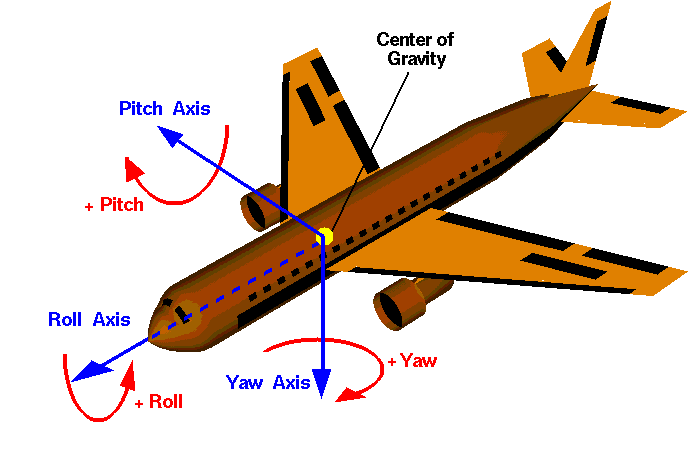
\includegraphics[scale=0.5]{imagens/rotations.png}

            \caption*{Fonte: \citeonline{NASA}.}

        \end{figure}
        
        O eixo nomeado de \textit{Yaw} ($\psi$) é definido como perpendicular as asas do avião, tem origem no centro de gravidade e é direcionado para baixo (via Figura \ref{fig:rotations}). O eixo \textit{Pitch} ($\theta$) é perpendicular ao eixo \textit{Yaw} e paralelo as asas da aeonave, com origem no centro de gravidade e tem a direção das asas.
        O eixo \textit{Roll} ($\phi$) é perpendicular aos outros eixos, com origem no centro de gravidade e é direcionado ao nariz da aeronave.
        
        Observando estes eixos e definindo no sensor inercial, para distinguir as letras que possuem movimento será necessário somente o eixo de rotação \textit{Roll}, como pode ser observado na Figura \ref{fig:mpu_eixos}.
        
        \begin{figure}[H]
        	\vspace{4mm}
            \centering
            \caption{Sensor inercial com o eixo de \textit{Roll} definido}
            \label{fig:mpu_eixos}
            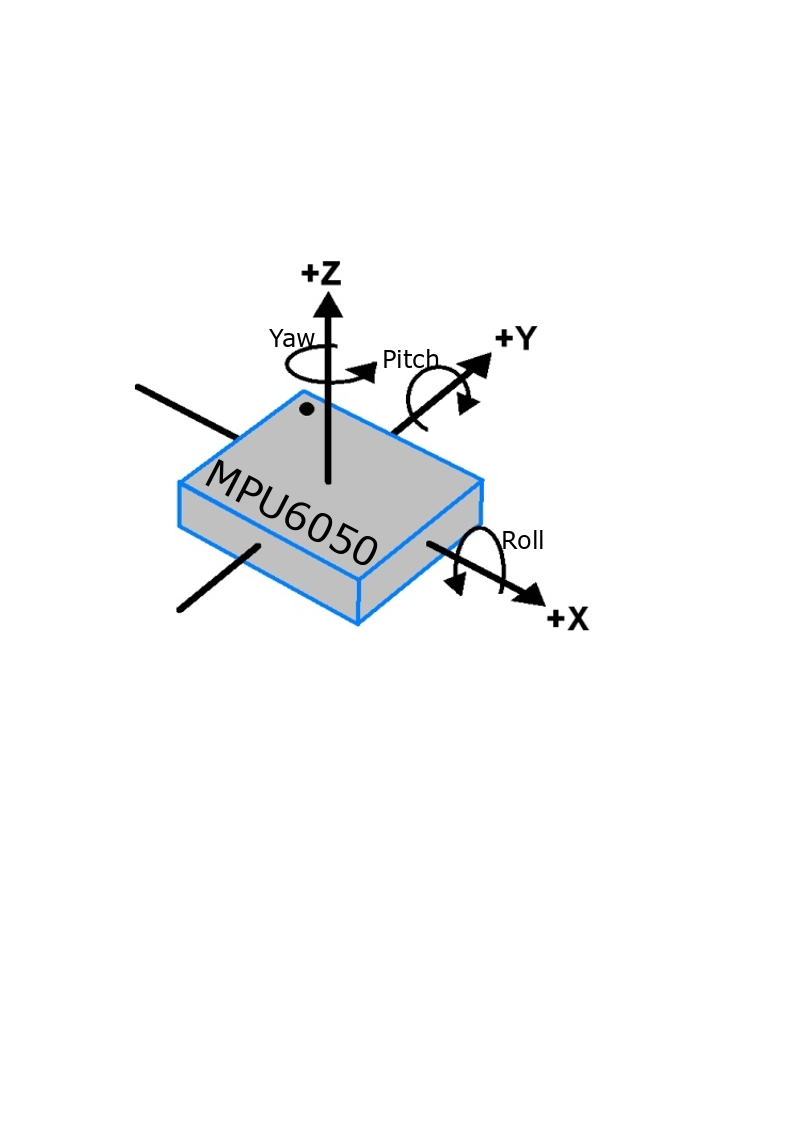
\includegraphics[scale=0.3, trim={4cm 14cm 6cm 7cm}, clip]{imagens/ypr2.png}
            \caption*{Fonte: Adaptado de \citeonline{eixos}.}
        \end{figure}
        
        
        De acordo com \citeonline{nxp:acell}, o acelerômetro dos celulares é utilizado para definir a orientação da tela utilizando o sistema de coordenadas tridimensionais. Logo é possível obter os eixos \textit{Pitch} e \textit{Roll} a partir dos valores dos 3 eixos do acelerômetro.
        
        Assumindo que o acelerômetro é orientado no campo gravitacional da terra $g$ e passa por aceleração linear $a_r$ medido no \textit{frame} de referência da terra $r$, terá uma saída dada por \cite{nxp:acell}:
        \begin{equation}
            G_p = 
            \begin{pmatrix}
                G_{px} \\
                G_{py} \\
                G_{pz}
            \end{pmatrix}    
             = R (g - a_r),
            \label{eq:ROLL1}
        \end{equation}
        onde $R$ é a matriz de rotação que descreve a orientação do acelerômetro com relação as coordenadas da terra.
        
        
        Supõe-se que o acelerômetro não tem aceleração linear ( necessário assumir isso para resolver a Equação \ref{eq:ROLL1} para a matriz de rotação $R$), quando houver presença de aceleração linear será adicionado um erro na estimação da orientação. Também assume-se que a orientação inicial do acelerômetro é plana com o campo gravitacional da terra e alinhado com o eixo $z$. Considerando isso, a saída $G_p$ do acelerômetro é demonstrada por \cite{nxp:acell} (medido em $g$):	
        
        \begin{equation}
            G_p = 
            \begin{pmatrix}
                G_{px} \\
                G_{py} \\
                G_{pz}
            \end{pmatrix}    
             = Rg = R.
             \begin{pmatrix}
                0 \\
                0 \\
                1
             \end{pmatrix}
            \label{eq:ROLL2}
            ,
        \end{equation}
        
    Para determinar os ângulos \textit{Yaw, Pitch} e \textit{Roll}, é necessário descrever as componentes da matriz de rotação $R$. As matrizes de rotação \textit{Yaw}($R_z(\psi)$), \textit{Pitch}($R_y(\theta)$) e \textit{Roll} ($R_x(\phi)$) transformam o vetor $G_p$ sobre uma rotação do sistema de coordenadas da Figura \ref{fig:mpu_eixos}
    para ângulos de \textit{Roll} ($\phi$), \textit{Pitch} ($\theta$), e \textit{Yaw} ($\psi$). Essas matrizes são expressas como \cite{nxp:acell}:
    \begin{equation}
        R_x(\phi) = 
        \begin{pmatrix}
            1 & 0 & 0\\
            0 & cos \phi & sin \phi\\
            0 & -sin \phi & cos \phi
        \end{pmatrix}
        \label{eq:ROLL3}
        ,
    \end{equation}
    
    \begin{equation}
        R_y(\theta) = 
        \begin{pmatrix}
            cos \theta & 0 & -sin \theta \\
            0 & 1 & 1\\
            sin \theta & 0 & cos \theta
        \end{pmatrix}
        \label{eq:ROLL4}
        ,
    \end{equation}
    ,
    \begin{equation}
        R_z(\psi) = 
        \begin{pmatrix}
            cos \psi & sin \psi & 0 \\
            -sin \psi & cos \psi & 0 \\
            0 & 0 & 1
        \end{pmatrix}
        \label{eq:ROLL5}
        .
    \end{equation}
    
    Existem seis possibilidades para ordenar essas três matrizes de rotação. Em princípio, todas são igualmente válidas \cite{nxp:acell}. Considerando isso e inicialmente o valor de $1g$ no eixo $z$, resulta em  \cite{nxp:acell}:
    
    \begin{equation}
        R_{xyz}.
        \begin{pmatrix}
        0 \\ 0 \\ 1
        \end{pmatrix}
        = R_x(\phi) R_y(\theta) R_z(\psi).
        \begin{pmatrix}
            0 \\ 0 \\ 1
        \end{pmatrix}
        \label{eq:ROLL6}
        .
    \end{equation}
    
    Fazendo a substituição e a multiplicação das matrizes das Equações \ref{eq:ROLL3}, \ref{eq:ROLL4}, e \ref{eq:ROLL5} na Equação \ref{eq:ROLL6} demonstra-se que  \cite{nxp:acell}:
    
    \begin{equation}
        \begin{pmatrix}
            cos \theta cos \psi & cos \theta sin \psi & -sin \theta \\
            
            cos \psi sin \theta sin \phi - cos \phi sin \psi & 
            cos\phi cos\psi + sin \theta sin \phi sin \psi &
            cos \theta sin \phi \\
            
            cos \phi cos\psi sin \theta  + sin\phi sin\psi &
            cos \phi sin \theta sin \psi - cos \psi sin \phi &
            cos \theta cos\phi 
            
        \end{pmatrix}
        .
        \begin{pmatrix}
            0 \\ 0 \\ 1
        \end{pmatrix}
        \label{eq:ROLL7}
        ,
    \end{equation}
    efetuando a multiplicação resulta na matriz:
    
    \begin{equation}
    = 
        \begin{pmatrix}
        -sin \theta \\ cos\theta sin \phi \\ cos\theta cos \phi
        \end{pmatrix}
        \label{eq:ROLL8}
        .
    \end{equation}
    
    Reescrevendo \ref{eq:ROLL8} com base no vetor $G_p$ resulta em:

    \begin{equation}
        \frac{G_p}{|| G_p ||}
        = 
        \begin{pmatrix}
            -sin \theta \\ cos\theta sin \phi \\ cos\theta cos \phi
        \end{pmatrix}
        \Rightarrow
        \frac{1}{\sqrt{G_{px}^2 + G_{py}^2 + G_{pz}^2}}
        \begin{pmatrix} 
            G_{px} \\ G_{py} \\ G_{pz} 
        \end{pmatrix}
        =
        \begin{pmatrix}
            -sin \theta \\ cos\theta sin \phi \\ cos\theta cos \phi
        \end{pmatrix}
        \label{eq:ROLL9}
        ,
    \end{equation}
    
    
    Resolvendo \ref{eq:ROLL9} para o eixo necessário para este trabalho, que é o \textit{Roll}, tem-se:
    \begin{equation}
        tan_{xyz} \phi =  \frac{G_{py}}{G_{pz}}
        .
        \label{eq:ROLL10}
    \end{equation}
    
    Utilizando os valores de $G_{py} = 0,082198$ e $G_{pz} = -0,887432$, a resolução de \ref{eq:ROLL10} pode ser tanto $-5.29$ ou $174.71$, uma vez que os valores de \textit{Roll} variam de -180º a 180. Para solucionar este problema se utiliza da função atan2, que automaticamente retorna o ângulo em radianos no quadrante correto baseado no sinal dos dois argumentos \cite{nxp:acell}. Finalmente, chega-se a expressão para calcular o \textit{Roll} do acelerômetro:

    \begin{equation}
        \phi_{xyz} = atan2(G_{py}, G_{pz}).
        \label{eq:ROLL11}
    \end{equation}

\section{Sensores Indutivos}
\label{sec:indutivo}

Como apresentado por \citeonline{INSTRUME}, sensores indutivos são dispositivos sem contato e utilizados geralmente 
para medição de posição. Utilizando o efeito de indução eletromagnética em um corpo condutor, é possível produzir 
corrente elétrica quando o campo magnético é variável ou quando é efetuado movimento em um campo estático. Considerando uma espira 
C, a corrente induzida pode ser representada por \cite{moyses}:

\begin{equation}
  i = \frac{-1}{R} \frac{d \Phi_c}{dt},
  \label{eq:I_indu}
\end{equation}
onde i é a corrente induzida, R é a resistência de uma espira C, e $\frac{d \Phi_c}{dt}$ é a variação de campo que atravessa a 
espira C. A existência dessa corrente na espira está associada uma força eletromotriz (fem) induzida descrita por \cite{moyses}:

\begin{equation}
  \varepsilon = Ri = -\frac{d\Phi_c}{dt},
  \label{eq:fem_ind}
\end{equation}
em que $\varepsilon$ é a fem induzida.
 
 Como neste trabalho são utilizadas pares de bobinas geradoras e sensoras é utilizado o efeito de indução mútua que é 
apresentado por \citeonline{Young}. Considerando duas bobinas vizinhas (vide Figura \ref{fig:Duasbob}). Uma corrente $i_1$ 
circulando na bobina 1 produz campo magnético \textbf{$\overrightarrow{B}$} e um fluxo magnético através da bobina 2. Quando 
$i_1$ varia, o fluxo magnético através da bobina 2 também varia, produzindo uma fem.

\begin{figure}[H]
	\vspace{4mm}
  \centering
  \caption{Exemplo de efeito de indução mútua}
  \label{fig:Duasbob}
  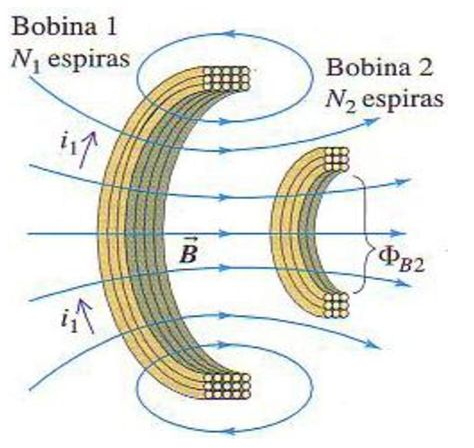
\includegraphics[scale=0.3]{imagens/InducaoMutua.png}
  \caption*{Fonte: \citeonline[p. 317]{Young}.}
\end{figure}


  A fem induzida na bobina 2 pode ser representada em termos da variação de corrente na bobina 1, conforme \cite{Young}:

\begin{equation}
  \varepsilon_2 = -M \frac{di_1}{dt},
  \label{eq:variacao}
\end{equation}
 onde $M$ é conhecida como indução mútua e depende das indutâncias das bobinas 1 e 2, assim como do acoplamento entre elas. Em 
termos de fluxos magnéticos, a indutância mútua pode ser obtida a partir de \cite{Young}:

\begin{equation}
  M =\frac{ N_2 \Phi_{B2}}{i_1} =  \frac{N_1\Phi_{B1}}{i_2},
 \label{eq:indutanciaMutua}
\end{equation}

em que $N_1$ e $N_2$ são os número de espiras das respectivas bobinas, $\Phi_{B1}$ e $\Phi_{B2}$ correspondem aos fluxos magnéticos nas bobinas 1 e 2 respectivamente, $i_1$ e $i_2$ são as correntes de cada uma das bobinas. 

Este princípio da indução é aplicado em transformadores, com circuitos CA para aumentar ou diminuir uma tensão de entrada. Um dos 
problemas 
envolvidos em transformadores é que a potência fornecida pela bobina fonte depende da resistência da fonte de carga do circuito 
conectado a outra bobina \cite{Young}.

Para solucionar este problema, considera-se a condição de ressonância, onde a impedância atinge o seu valor mínimo e a corrente 
atinge o valor máximo. Para isso, é necessário adicionar um capacitor ao circuito da bobina. Desta forma, a frequência de ressonância
do circuito LC é dada por:
\begin{equation}
  f_0 = \frac{1}{2 \pi \sqrt{LC}},
 \label{eq:freqResso}
\end{equation}
$L$ é o indutor e $C$ é o capacitor. A Figura \ref{fig:transform} demonstra o 
esquemático do sensor e gerador projetados para operar em ressonância.\\


\begin{figure}[H]
  \centering
 	\vspace{4mm}
 	    \caption{Topologia dos circuitos de sensoriamento}
 	    \label{fig:transform}
    \begin{circuitikz} 
      \draw
      %circuito esquerda
      (0,0) to [short] (2,0)
      to [C, l_=$C_2$] (2,2)
      to [short] (0,2)
      (2,0) to [short] (4,0)
      to [L,l_=$L_2$] (4,2)
      to [short] (2,2)


      %circuito direita
      (6,2) to [R,l=$R_1$] (8,2)
      to [C, l=$C_1$] (10,2)
      (6,2) to [L, l=$L_1$] (6,0)
      to [short] (10,0)
      ;

      \draw [decorate, decoration={brace, amplitude=10pt, mirror, raise=4pt}, yshift=0pt] (0,0) -- (4,0)  node 
      [midway, yshift=-0.8cm]{sensor};
      \draw [decorate, decoration={brace, amplitude=10pt, mirror, raise=4pt}, yshift=0pt] (6,0) -- (10,0) node 
      [midway, yshift=-0.8cm] {gerador};
    \end{circuitikz}
	
    \caption*{Fonte: \citeonline[p. 67]{RUANI}.}

\end{figure}

Para o projeto do valor de $C$, foi assumida a frequência de ressonância pré-definida de $100\textrm{ }kHz$ e a indutância das bobinas desenvolvidas por 
\citeonline{RUANI}. Isolando-se $C$ em \ref{eq:freqResso} obtem-se:	

\begin{equation}
 C = \frac{1}{4 \pi^2 f_0^2 L}.
 \label{eq:capa}
\end{equation}

\section{Reconhecimento de padrões}
Para \citeonline{Haykim_ingles}, o reconhecimento de padrões é formalmente definido como o processo que um determinado 
sinal/padrão recebido é classificado para uma das classes predefinidas. A Figura \ref{fig:fluxogramadesign}  exibe um diagrama 
dos componentes de um sistema típico de reconhecimento de padrões. Para entender o problema de projeto de um sistema, é 
necessário o entendimento dos problemas que cada um desses componentes resolve \cite{PatternDuda}.\\

\begin{figure}[H]
  
	\centering
	\caption{Modelo de sistemas de classificações de padrões}
	\label{fig:fluxogramadesign}
	\begin{tikzpicture}[node distance=1cm, >=triangle 60,
	estilo/.style={draw, rectangle, minimum width=5cm, minimum height=1cm, text centered, line width=0.07cm}]
		
		\node[draw=none] 			(A)  {entrada};
		\node[draw, estilo, above=of A] 	(B)  {detecção};
		\node[draw, estilo, above=of B] 	(C)  {segmentação};
		\node[draw, estilo, above=of C] 	(D)  {extração de característica};
		\node[draw=red, estilo, above=of D] 	(E)  {classificação};
		\node[draw, estilo, above=of E] 	(F)  {pós-processamento};
		\node[draw=none, above= of F] 		(G)  {decisão};
		
		\node[draw=none, right=of F, xshift=2cm] 			(H)  {custos};
		\node[draw=none, right=of F, yshift=-1cm,xshift=2cm,align=left] 	(I)  {ajustes para \\ contextos};
		\node[draw=none, right=of E, yshift=-1cm,xshift=2cm,align=left] 	(J)  {ajustes para \\ características 
faltantes};
		
		\draw[->, line width=0.03cm]  (A) -- (B);
		\draw[->, line width=0.03cm]  (B) -- (C);
		\draw[->, line width=0.03cm]  (C) -- (D);
		\draw[->, line width=0.03cm]  (D) -- (E);
		\draw[->, line width=0.03cm]  (E) -- (F);
		\draw[->, line width=0.03cm]  (F) -- (G);
		
		\draw[->, gray, line width=0.03cm]  ($(C.south) + (0.8cm, 0)$) -- ($(B.north) + (0.8cm,0)$);
		\draw[->, gray, line width=0.03cm]  ($(D.south) + (0.8cm, 0)$) -- ($(C.north) + (0.8cm,0)$);
		\draw[->, gray, line width=0.03cm]  ($(E.south) + (0.8cm, 0)$) -- ($(D.north) + (0.8cm,0)$);
		\draw[->, gray, line width=0.03cm]  ($(F.south) + (0.8cm, 0)$) -- ($(E.north) + (0.8cm,0)$);			
		
		\draw[->, red, line width=0.03cm]  (H.west) -- ($(F.east) + (0, 0.2cm)$);
		\draw[->, red, line width=0.03cm]  (I.west) -- ($(F.east) - (0, 0.2cm)$);
		\draw[->, red, line width=0.03cm]  ($(I.west) - (0, 0.2cm)$) -- ($(E.east) + (0, 0.2cm)$);
		\draw[->, red, line width=0.03cm]  (J.west) -- ($(E.east) - (0, 0.2cm)$);
	

	\end{tikzpicture}
	\caption*{Fonte: \citeonline{PatternDuda}.}
\end{figure}


A entrada corresponde a um fenômeno que se deseja avaliar. A detecção converte esse fenômeno em um sinal elétrico, por exemplo, sendo representado por um sensor que no caso do presente trabalho corresponde aos sensores indutivos e acelerômetro. As dificuldades variam de acordo com as limitações sensor, tais como resolução, sensividade, ruído, latência
\cite{PatternDuda}.
  A segmentação separa os objetos detectados pelo sensor de outros objetos ou do cenário. Tomando como base o sinal do acelerômetro, a segmentação é utilizada para separar onde começa o sinal de uma letra e onde termina \cite{PatternDuda}.

  O objetivo tradicional da extração de característica é caracterizar um objeto para ser identificado por valores que podem ser 
  mensurados, em que, esses valores são muito similares para objetos de mesma categoria e muito distantes para objetos de 
  categorias diferentes. Isso leva a ideia de procurar características marcantes que são invariantes para transformações de 
entrada \cite{PatternDuda}.

  O papel do componente classificador em um sistema completo é usar as características escolhidas pela extração e atribuir este 
  objeto a uma classe. Como a classificação perfeita é muitas vezes impossível, uma tarefa mais geral do classificador é definir 
  a porcentagem que um objeto pertença a uma classe \cite{PatternDuda}.

  No pós-processamento são levados em conta as considerações, como os efeitos do contexto e o custo dos erros para determinar a 
ação apropriada. Uma simples medida de desempenho é a porcentagem de erros, a qual se refere a quantidade de classificações para 
uma classificação incorreta. Nesta etapa também pode ser analisada a eficiência de se utilizar múltiplos classificadores, 
adicionando um para a detecção dos gestos por uma câmera, por exemplo \cite{PatternDuda}.
  
  
\section{Redes Neurais}
	Conforme \citeonline{Redes_cursopratico}, redes neurais são estruturas baseadas no sistema nervoso dos seres vivos que possuem a capacidade de armazenar e manter conhecimento.

\subsection{Arquitetura de um neurônio}
O neurônio é uma unidade de processamento de informação fundamental para a operação de uma rede neural, sendo a base para redes neurais artificiais \cite{haykin}. Na Figura \ref{fig:neuronio}, pode-se notar a presença de três elementos: o conjunto de pesos sinápticos; função de ativação; e a junção aditiva.
\begin{figure}[H]
	\vspace{4mm}
	\centering
	\caption{Modelo não linear de um neurônio}
	\label{fig:neuronio}
	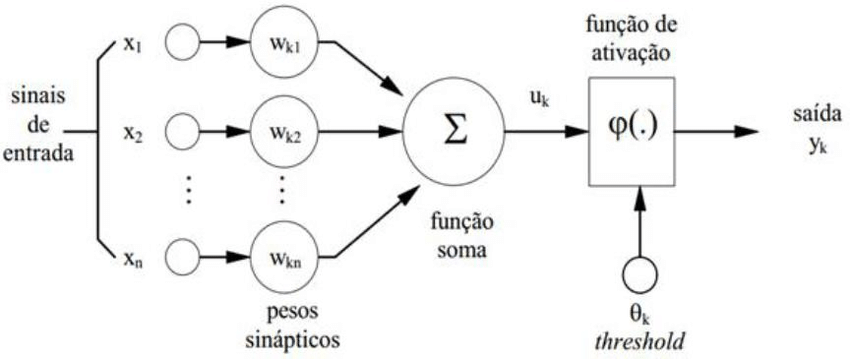
\includegraphics[scale=0.35]{imagens/neuronio}
	\caption*{Fonte: \citeonline[p. 38]{haykin}.}
\end{figure}

De acordo com \citeonline{Redes_cursopratico}, os pesos sinápticos são os valores que servirão para ponderar cada uma das variáveis de entrada da rede, permitindo quantificar as suas relevâncias em relação a funcionalidade do respectivo neurônio. As entradas, após serem ponderadas, são somadas pela junção aditiva ou combinador linear, que é um somador dos valores de entrada ponderados pelos respectivos pesos sinápticos. Esse processo é representado por \cite{haykin}:

\begin{equation}
	u_k = 	\sum_{j=1}^{n}.w_{kj}x_j,
\end{equation}
onde $x_j$ são os sinais de entrada, $w_{kj}$ são os pesos sinápticos, $u_k$ é a saída do combinador linear.

A função de ativação ou função restritiva é aplicada para restringir a amplitude de saída de um neurônio. Tipicamente, a amplitude de saída de um neurônio é escrita como o intervalo unitário fechado $[0, 1]$ ou alternativamente $[-1, 1]$. A função de ativação recebe a saída do combinador linear, conforme \cite{haykin}:

\begin{equation}
	y_l = \varphi(u_k + b_k),
\end{equation}
onde $y_k$ é o sinal de saída do neurônio e $b_k$ é o \textit{bias}. O \textit{bias} tem o efeito de aumentar ou diminuir a entrada líquida da função de ativação \cite{haykin}. O valor do bias é ajustado da mesma forma que os pesos sinápticos. O bias possibilita que um neurônio apresente uma saída não nula mesmo que todas as suas entradas sejam nulas \cite{redesemc}.

\subsection{Funções de ativação}
\label{sec:funcao}
A função de ativação, representada por $\varphi(v)$, define a saída em termos do potencial de ativação $v$. Os principais tipos de funções de ativação consistem da função limiar, representada na Figura \ref{fig:limiar}, e da função sigmoide, mostrada na Figura \ref{fig:sigmoide} \cite{haykin}.

\begin{figure}[H]
	\vspace{4mm}
	\centering
	\caption{Função de ativação limiar}
	\label{fig:limiar}
	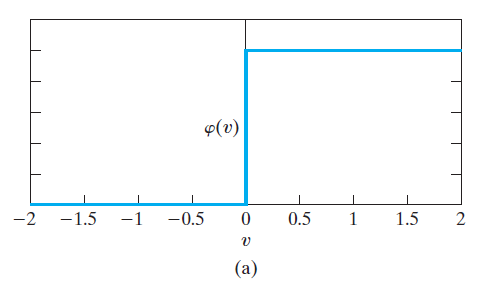
\includegraphics[scale=0.5]{imagens/limiar}
	\caption*{Fonte: \citeonline[p. 39]{haykin}.}
\end{figure}

\begin{figure}[H]
	\vspace{4mm}
	\centering
	\caption{Função de ativação sigmoide}
	\label{fig:sigmoide}
	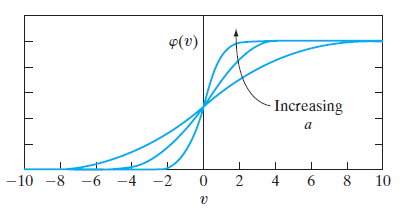
\includegraphics[scale=0.7]{imagens/sigmoide}	
	\caption*{Fonte: \citeonline[p. 39]{haykin}.}
\end{figure}

A função sigmoide é a forma mais comum de função de ativação para a construção de redes neurais artificiais, sendo definida como uma função estritamente crescente que exibe um balanceamento adequado entre comportamento linear e não linear. Dois exemplos de funções de ativação sigmoides são a função logística \cite{haykin}:

\begin{equation}
	\varphi(v) = \frac{1}{1 + exp(-av)},
\end{equation}
e a função tangente hiperbólica:

\begin{equation}
	\varphi(v) = tanh(v).
\end{equation}

\subsection{Arquitetura de uma rede neural}

A arquitetura de uma rede neural artificial define  a forma como seus diversos neurônios estão arranjados, uns em relação aos outros \cite{Redes_cursopratico}.

Nas redes \textit{feedfoward} camada única possuí uma camada de entrada e que se projeta sobre a camada de saída dos neurônios, mas não vice-versa \cite{haykin}. Essa rede é ilustrada na Figura \ref{fig:camadaUnica}.

\begin{figure}[H]
	\vspace{4mm}
	\centering
	\caption{Arquitetura de camada única}
	\label{fig:camadaUnica}
	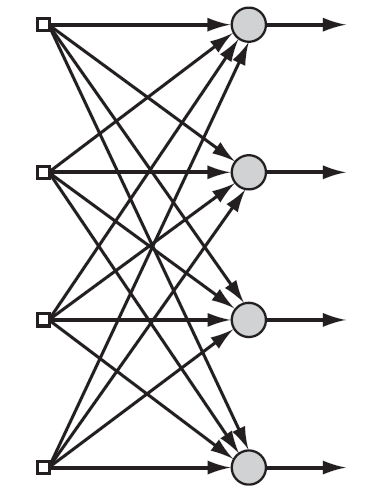
\includegraphics[scale=0.5]{imagens/rede_single}
	\caption*{Fonte: \citeonline[p. 47]{haykin}.}
\end{figure}


De acordo com \citeonline{Redes_cursopratico}, as redes \textit{feedfoward} multicamadas são constituídas de uma ou mais camadas escondidas de neurônios, conforme ilustrado na Figura \ref{fig:camadamultipla}. A função dos neurônios ocultos é intervir entre a entrada externa e a saída da rede de maneira útil. Adicionando-se uma ou mais camadas ocultas, a rede torna-se capaz de extrair características de ordem elevada \cite{haykin}.
\begin{figure}[H]
	\vspace{4mm}
	\centering
	\caption{Arquitetura de múltiplas camadas totalmente conectada}
	\label{fig:camadamultipla}
	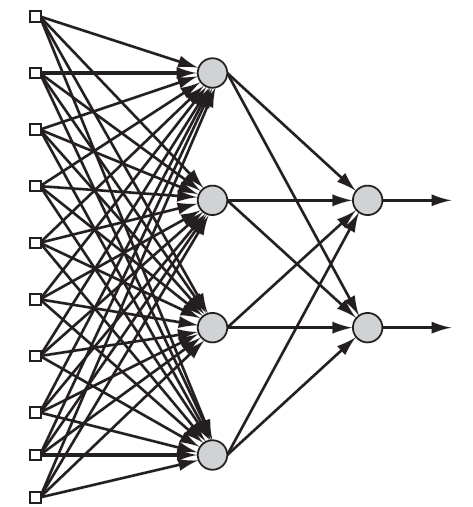
\includegraphics[scale=0.5]{imagens/rede_fully}
	\caption*{Fonte: \citeonline[p. 48]{haykin}.}
\end{figure}

\subsection{Aprendizagem supervisionada}
Conforme \citeonline{Redes_cursopratico}, a estratégia de treinamento supervisionado ou aprendizagem supervisionada consiste em se ter disponível, considerando cada amostra dos sinais de entrada, as respectivas saídas desejadas. Suponha um professor que conhece o ambiente no qual a rede será exposta. Retirando ambos do ambiente e expondo-os ao um vetor de treinamento, o professor é capaz de fornecer a saída correta para a rede neural. Então os parâmetros da rede são ajustados sob a influência combinada do vetor de treinamento e do sinal de erro. O sinal de erro é a diferença entre a resposta desejada e a resposta da rede \cite{haykin}.

Esse ajuste é feito passo a passo, transferindo o conhecimento do professor para a rede, da forma mais completa possível, e quando essa condição é alcançada, pode-se dispensar o professor e deixar a rede neural atuar sozinha \cite{haykin}.

\begin{figure}[H]
	\vspace{4mm}
	\centering
	\caption{Diagrama de aprendizado supervisionado}
	\label{fig:aprendizado}
	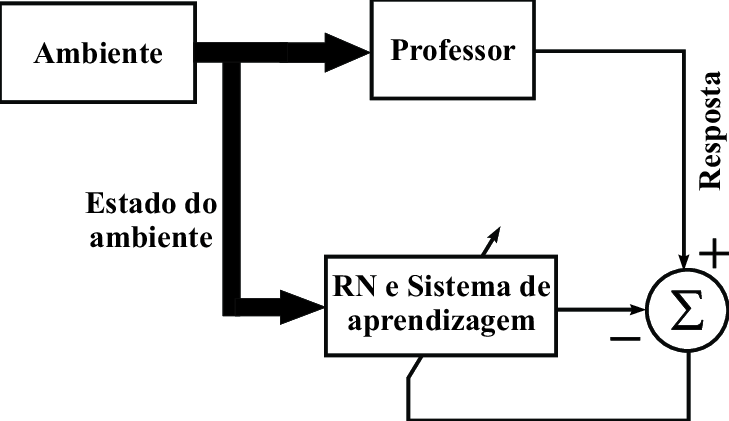
\includegraphics[scale=0.3]{imagens/aprendizado}
	\caption*{Fonte: \citeonline[p. 88]{haykin}.}
\end{figure}

\subsection{O algoritmo \textit{backpropagation}}
Em resumo, o algoritmo de retropropagação pode ser descrito em cinco etapas:

\begin{enumerate}
	\item Inicialização: arbitram-se valores aleatórios aos pesos sinápticos e níveis de \textit{bias}, em uma distribuição uniforme, cuja média deve ser zero \cite{redesemc}.

\item Apresentação dos exemplos: apresenta-se uma época de exemplos a rede. Para cada exemplo, realiza-se uma propagação dos sinais e a retropropagação dos erros com a correção dos pesos e níveis de \textit{bias} \cite{redesemc}.

\item Propagação: aplica-se à camada de entrada da rede o vetor de sinais de entrada e calcula-se a saída para todos os neurônios até a camada de saída, em seguida se calcula o erro para cada neurônio de saída \cite{redesemc}.

\item Retropropagação: calcula-se os ajustes dos pesos daquela camada bem como o \textit{bias}, os quais devem ser somados com os valores atuais. O processo segue até se ajustar os valores de pesos e \textit{bias} da camada de entrada \cite{redesemc}.

\item Iteração: apresentam-se novas épocas de exemplos de treinamento para a rede de forma aleatória até que seja satisfeito o critério de parada \cite{redesemc}.

\end{enumerate}


%Materiais e Metodos
\chapter{Materiais e Métodos}
Neste capítulo são apresentados os materiais necessários para o desenvolvimento deste projeto bem como todos os procedimentos seguidos para levar os resultados apresentados.

\section{Materiais}
    No presente trabalho foram utilizados diversos materiais e ferramentas computacionais, sendo que os principais compreendem:
	\begin{itemize}
		\item Placa de desenvolvimento com microcontrolador STM32F103C8T6;
		\item Módulo \textit{display} LCD 16x2 HD44780;
		\item Luva de sensores construída manualmente;
		\item Sensor inercial MPU-6050;
		\item Circuito condicionador de sinal;
		\item IDE de programação para família de microcontroladores STM32(Atollic);
		\item Depurador/programador ST-Link/V2;
		\item Interpretador da linguagem Python.
	\end{itemize}

	
	\subsection{Placa de desenvolvimento com microcontrolador STM32F103C8T6}
	
		A referida placa de desenvolvimento, ilustrada na Figura \ref{fig:micro}, possui um microcontrolador ARM-Cortex M3  de 32 bits com 20kB de memória SRAM e e 64 kB de memória flash. Ainda contém2 conversores A/D (Analógico para digital) de 12 bits, 3 temporizadores de propósito geral e até 37 portas de entrada e saída tolerantes a 5V \cite{STM32F103}.
        
        \begin{figure}[H]
            \centering
            \caption{Microcontrolador STM32F103C8T6}
            \label{fig:micro}
            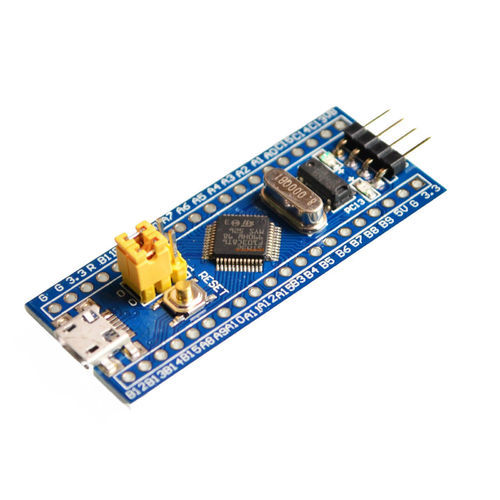
\includegraphics[scale=0.5]{imagens/micro.jpg}
            \caption*{Fonte: \citeonline{indiamart}.}

        \end{figure}
        
	\subsection{Módulo \textit{display} LCD 16x2 HD44780}
	
	    O módulo HD44780 \textit{display} de matrizes de pontos feito é com cristal liquido que pode reproduzir alfanuméricos, caracteres japoneses e símbolos customizados. Pode ser configurado para operar com transferência de 8 bits ou 4 bits. Todas as operações efetuadas para manipulação do \textit{display} são feitas na memória do controlador interno, sendo fornecido um driver transforma as informações escritas na memória para a tela de cristal liquido. O referido \textit{display} tem compatibilidade de pinagem com outros lcds de 16x2 para ser facilmente trocado caso haja necessidade. A baixa tensão de operação (2.7V até 5.5V) permite que o \textit{display} seja utilizado em sistemas ligados a bateria \cite{hitachi}.
    	Na Figura \ref{fig:hd44780} está o \textit{display} HD44780.
    	
    	\begin{figure}[H]
    	    \centering
     	    \caption{\textit{Display} LCD 16x2 de cristal líquido HD44780}
      	    \label{fig:hd44780}
    	    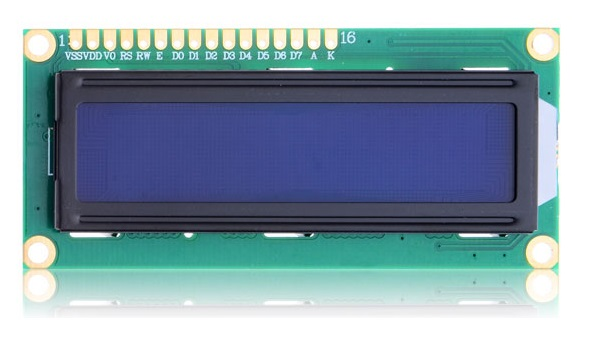
\includegraphics[scale=0.5]{imagens/hd44780.jpg}
    	    \caption*{Fonte: \citeonline{filipeflopHD}.}

    	\end{figure}
	
	\subsection{Sensor inercial MPU-6050}
    	O dispositivo MPU6050 é um sensor inercial de 6 eixos integrados que combina 3 eixos de giroscópio e 3 eixos de acelerômetro, e conta com um processador digital de movimentos, isso tudo em  um encapsulamento de 4x4x0,9 mm. Utilizado com comunicação I2C, o sensor aceita entradas de um compasso externo de 3 eixos para retornar uma fusão de coordenadas de movimento de 9 eixos \cite{mpu6050}.
        
        O dispositivo MPU6050 também possui internamente 3 conversores A/D (Analógico para digital) de 16 bits para giroscópio e 3 conversores A/D para acelerômetro afim de converter as entradas analógicas dos sensores. A escala de operação do acelerômetro é programável e pode ser escolhida entre  ±2g, ±4g, ±8g, e ±16g. O mesmo ocorre para o giroscópio, que tem as escalas de operação de ±250, ±500, ±1000, e ±2000°/sec \cite{mpu6050}. A Figura \ref{fig:mpu6050} ilustra a placa com o sensor MPU-6050 utilizada no presente projeto.

        \begin{figure}[H]
        	\vspace{4mm}
            \centering
            \caption{Sensor inercial MPU6050}
            \label{fig:mpu6050}
            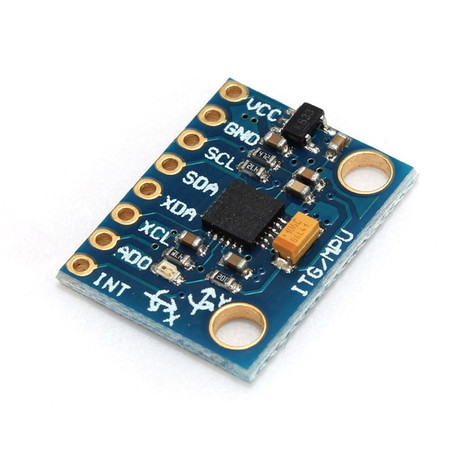
\includegraphics[scale=0.3]{imagens/mpu6050.jpg}
            \caption*{Fonte: \citeonline{filipeflopHD}.}

        \end{figure}
        
        
        \subsection{Conjunto de luva e circuito de condicionamento de sinais}
        A luva sensora, demonstrada na Figura \ref{fig:luva}, contém as bobinas sensoras e geradoras, todas ligadas ao um conector. 
\begin{figure}[H]
   	\vspace{4mm}
   	\centering
   	\caption{Luva sensora desenvolvida por \citeonline{RUANI}}
   	\label{fig:luva}
   	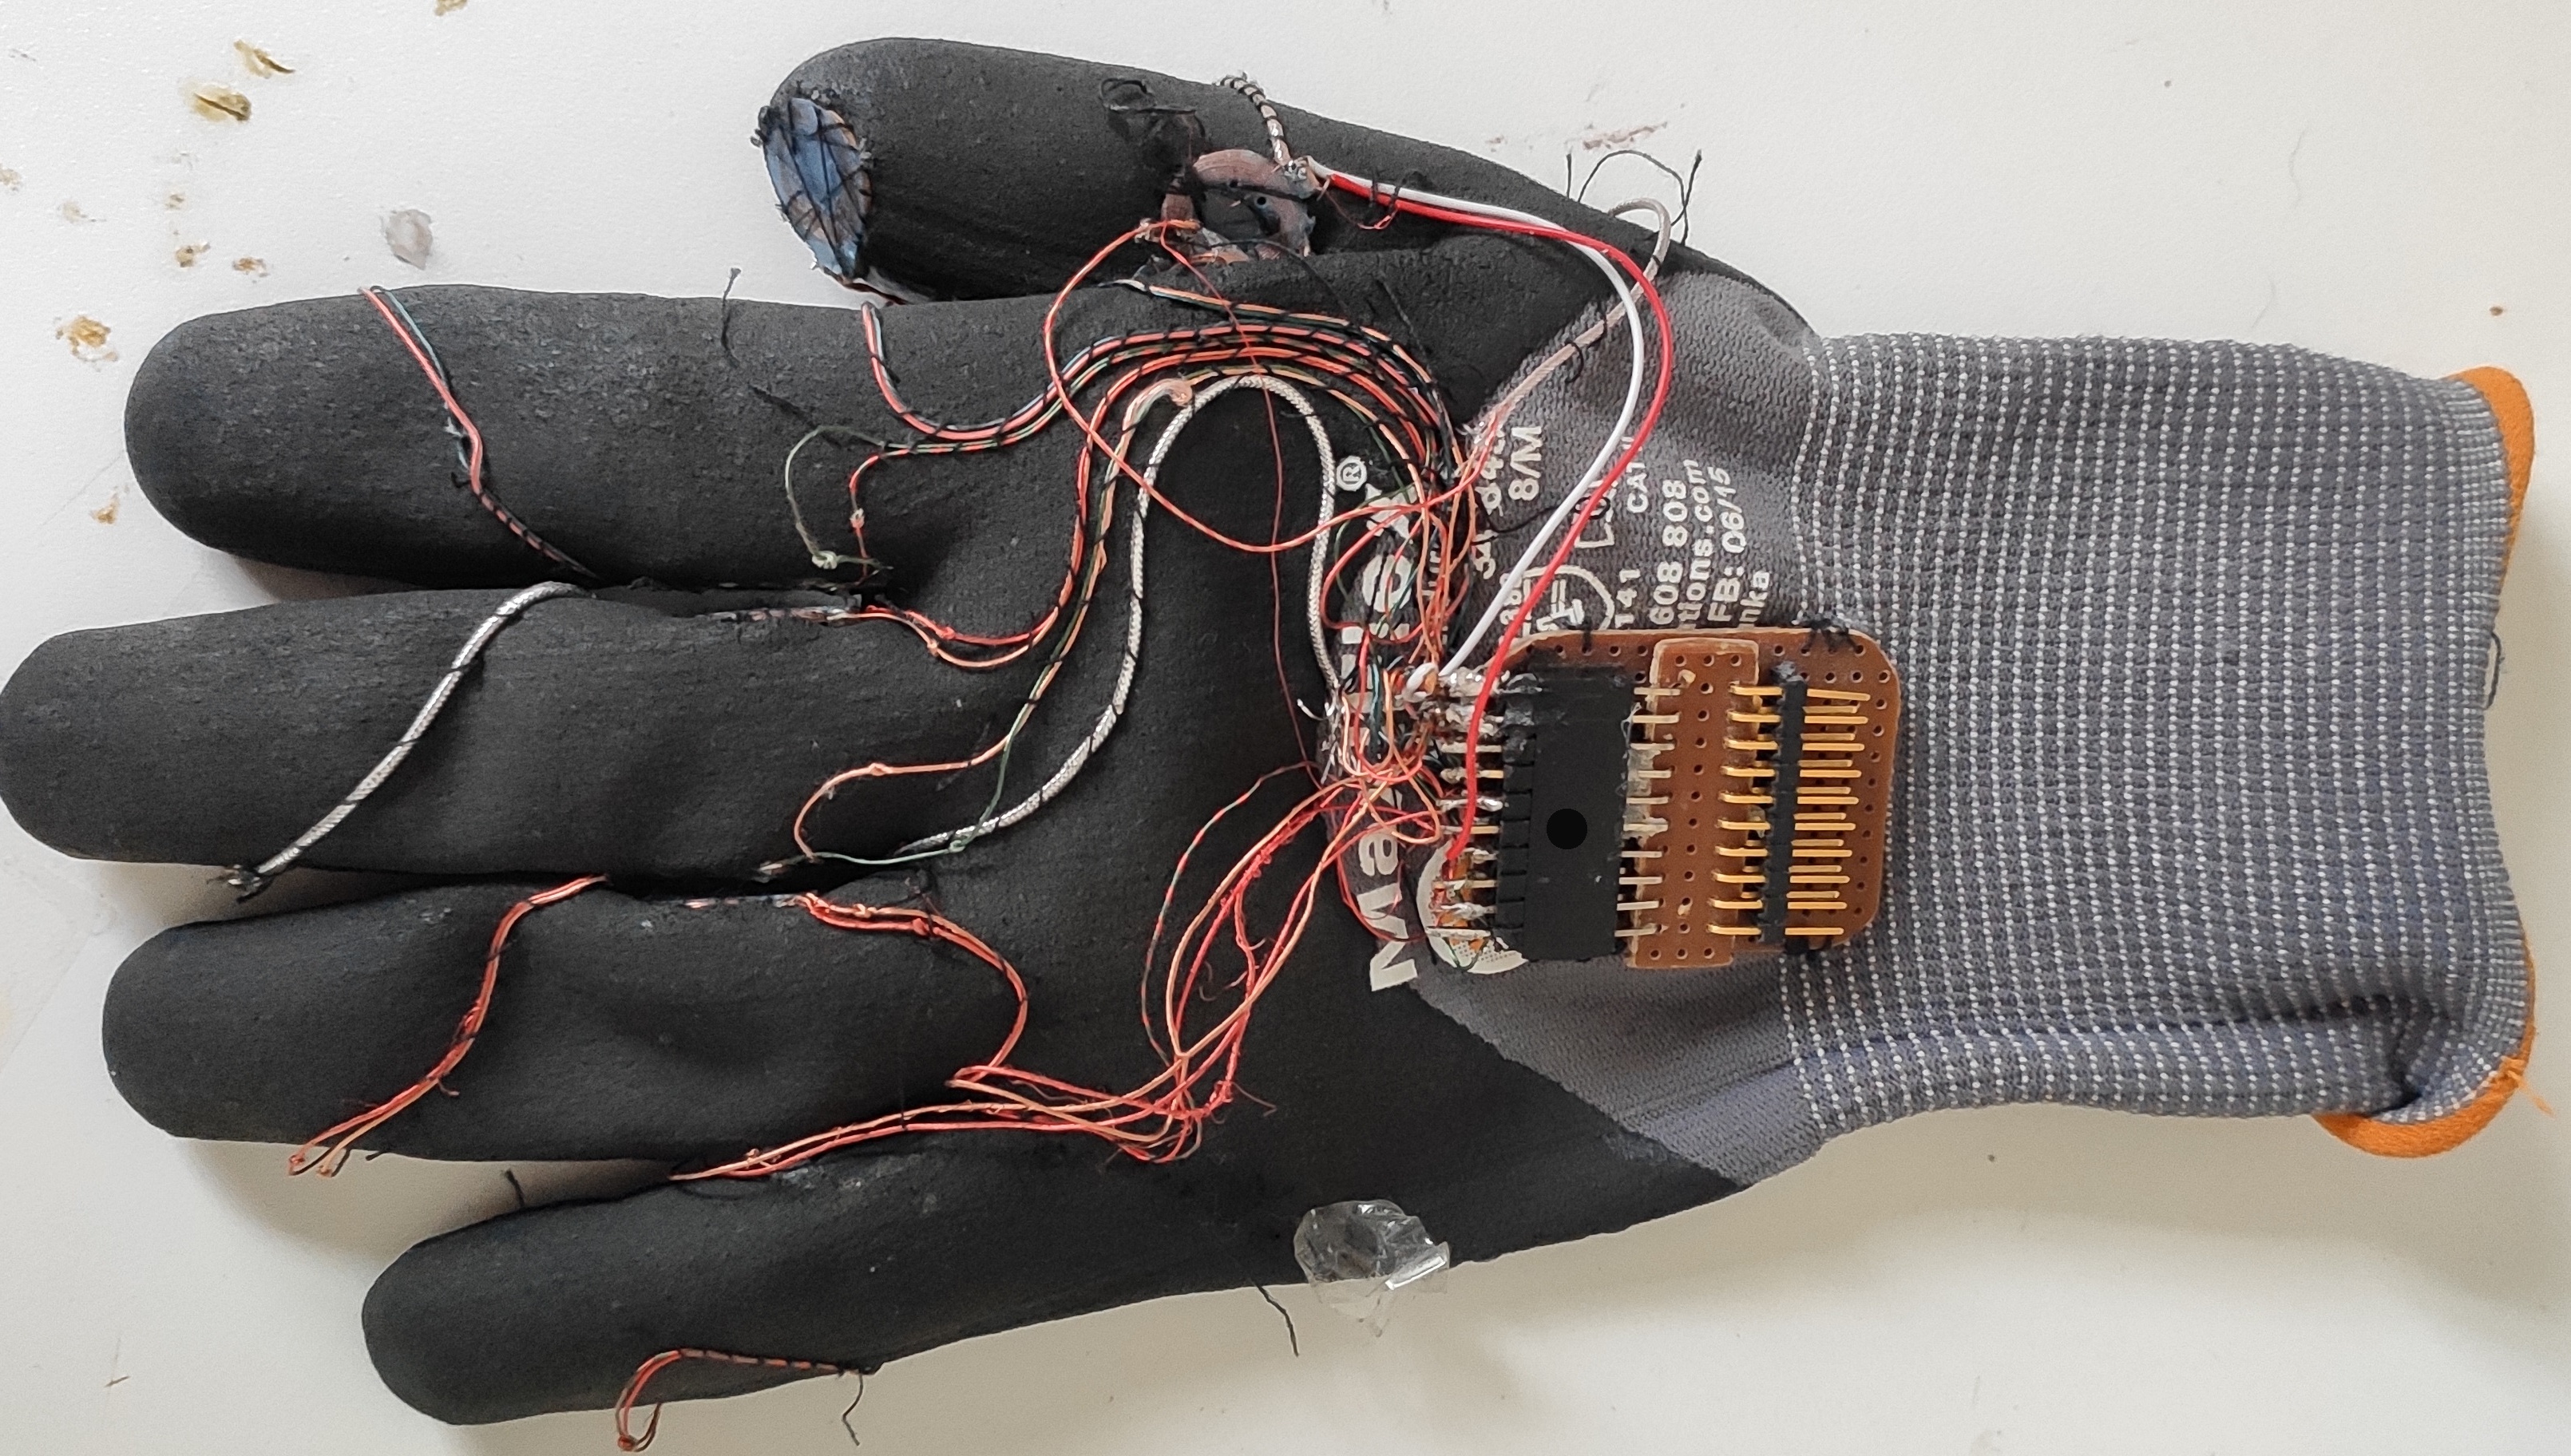
\includegraphics[scale=0.10]{imagens/luva_so.jpg}
   	\caption*{Fonte: Autoria própria.}
\end{figure}

A luva e conectada a placa de processamento de sinais das bobinas da Figura \ref{fig:placa1}. O funcionamento desta placa foi demonstrado na sessão \ref{sec:placa}. 

\begin{figure}[H]
   	\vspace{4mm}
   	\centering
   	\caption{Placa para recepção e processamento dos sinais vindos do sensor indutivo}
   	\label{fig:placa_in1}
   	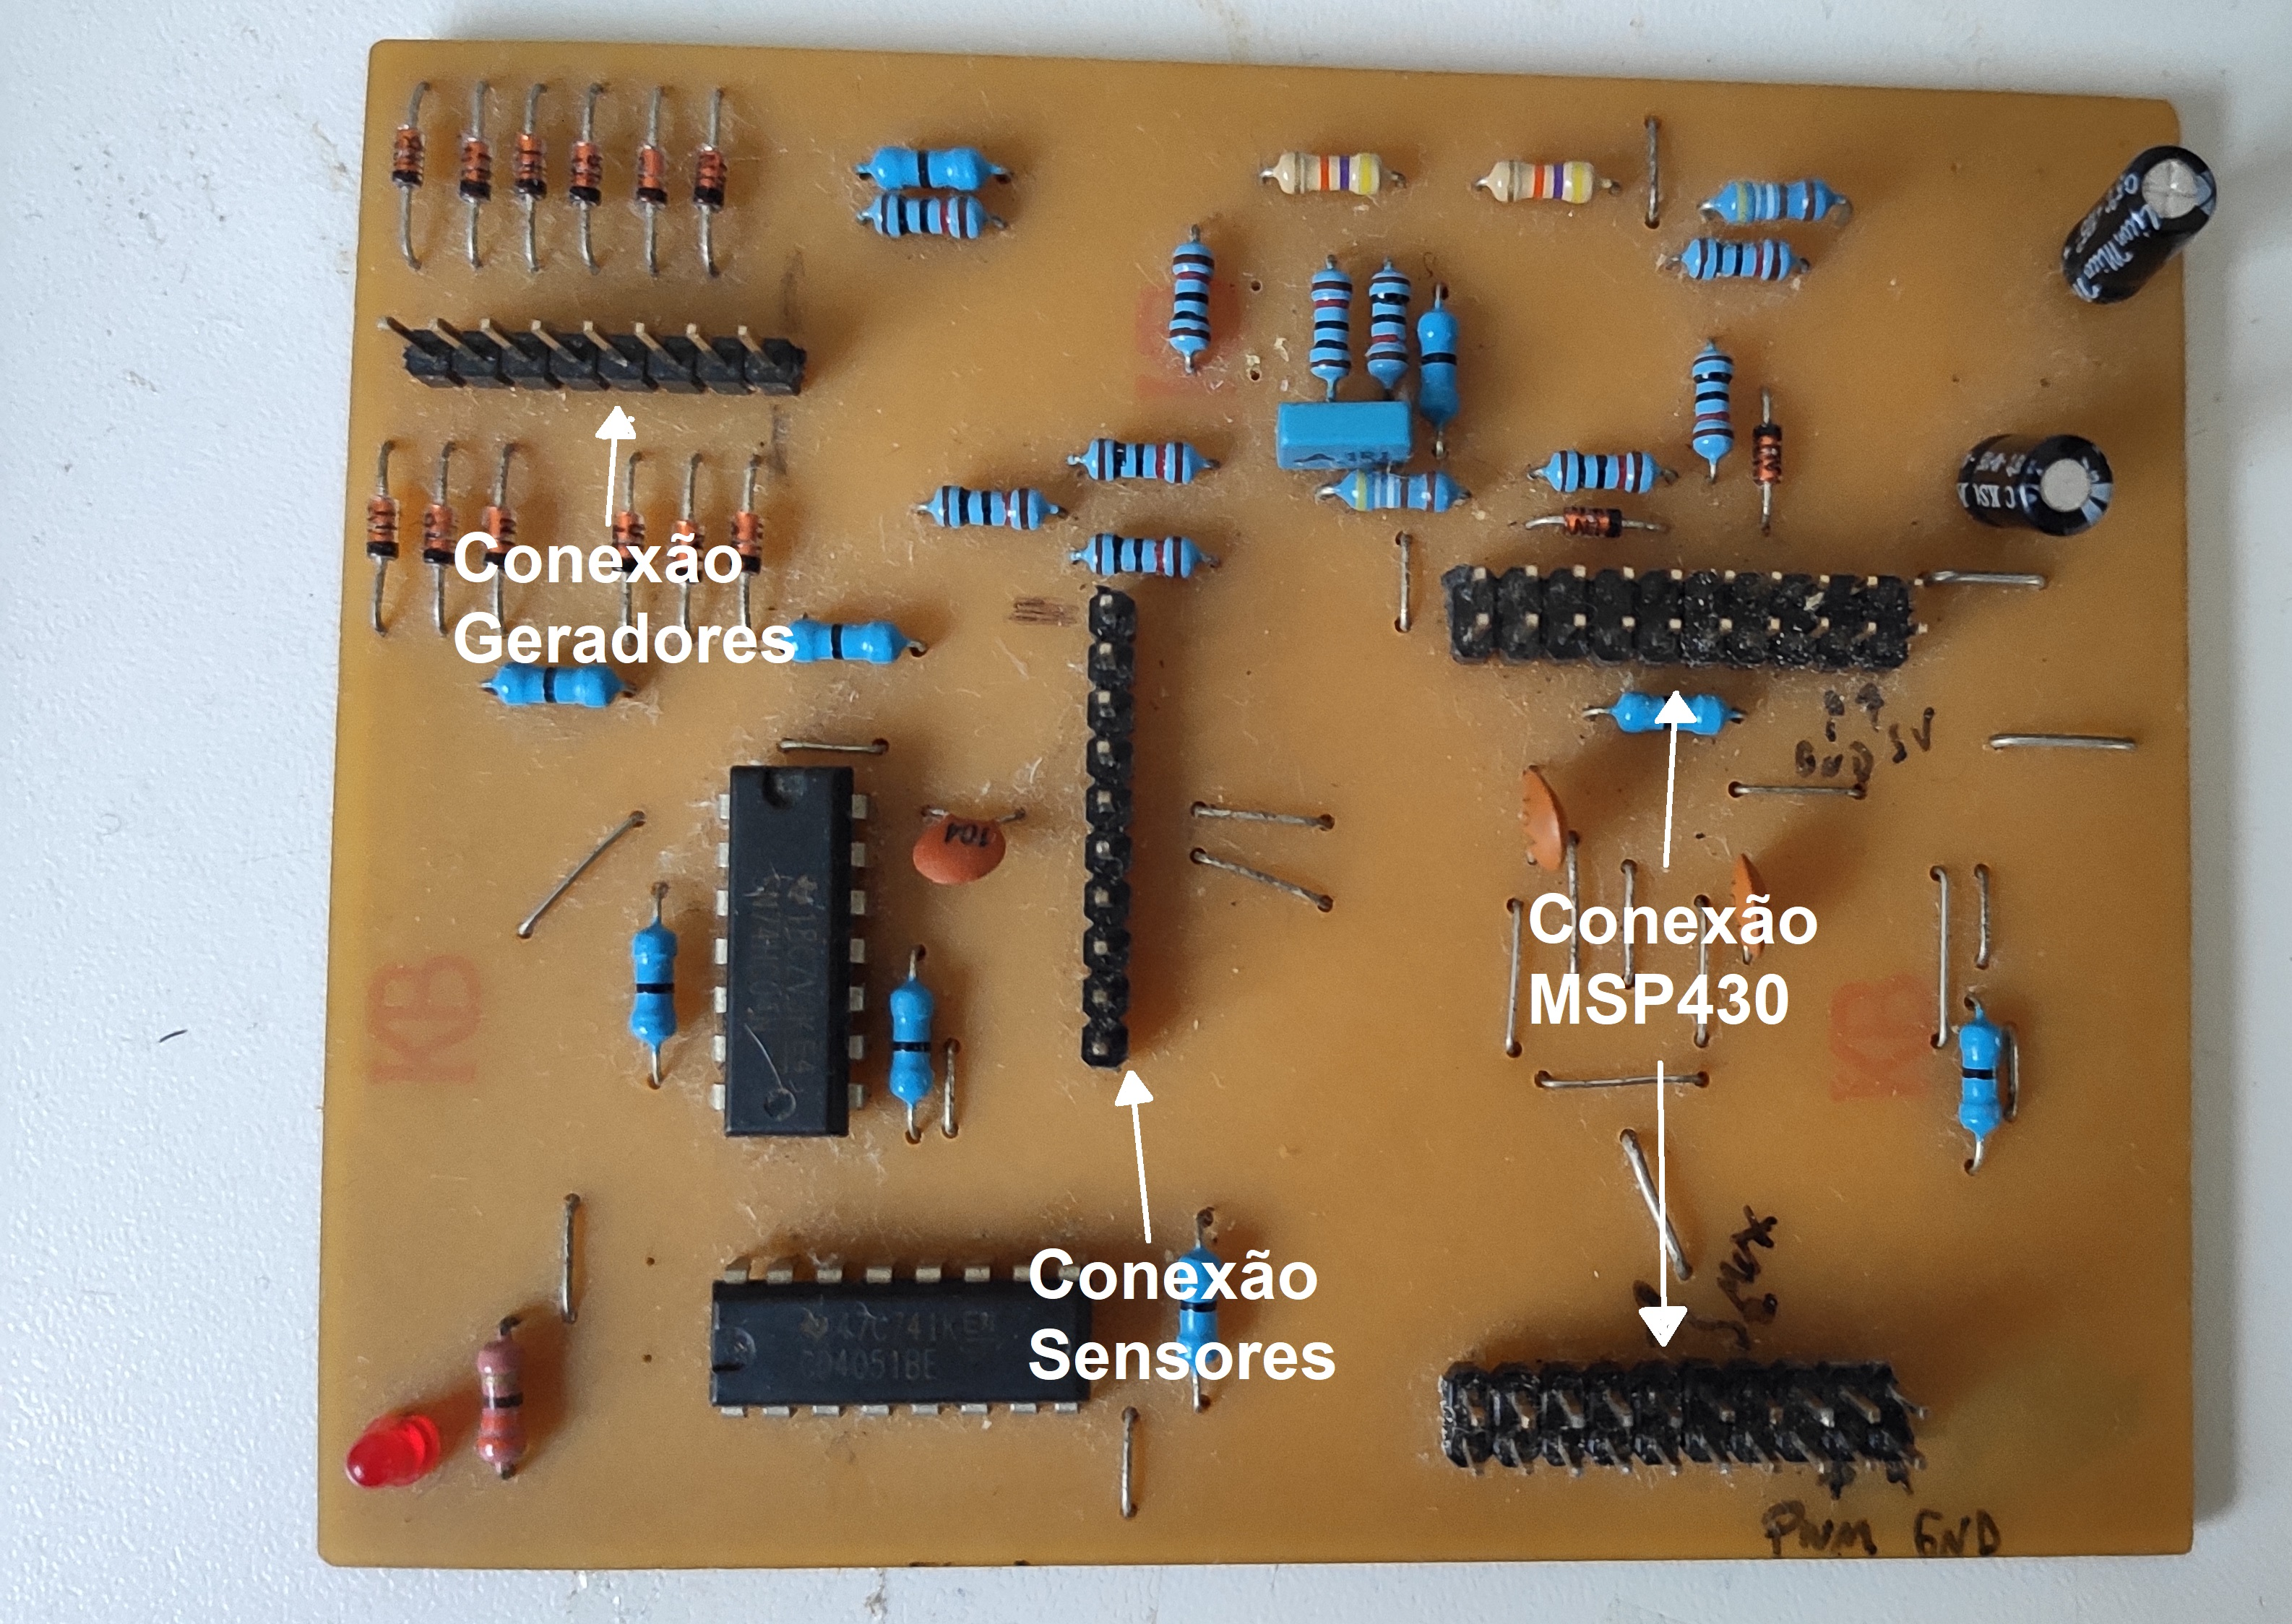
\includegraphics[scale=0.10]{imagens/placa_ruani.jpg}
   	\caption*{Fonte: Autoria própria.}
\end{figure}
	
A conexão é para o microcontrolador MSP430F5529, onde será encaixada uma placa de adaptação para o microcontrolador STM32F103C8T6.        
\section{Método}
A metodologia deste trabalho foi separada em compreensão do funcionamento e transferência do código para o novo microcontrolador, implementação do sensor inercial, processamento dos sinais, treinamento das redes neurais, e implementação das redes já treinadas no microcontrolador.

\subsection{Transferência do trabalho para o novo microcontrolador}
\label{sec:transf}
Primeiramente, foi necessário a análise do sistema já implementado em um trabalho anterior para conhecer o funcionamento como um todo.
Sendo feito a análise da resposta dos sensores indutivos, e fluxo do programa implementado. Após analisado o código, a estrutura física da luva, e funcionamento do sistema de condicionamento de sinais, foi feita a implementação no novo microcontrolador ARM. Foi utilizado o \textit{software} STM32CubeMX, para realizar as configurações dos periféricos de forma visual. A Figura \ref{fig:cubePinagem} mostra os pinos configurados no \textit{software}.

\begin{figure}[H]
	\centering
	\vspace{4mm}
		\caption{Pinos do microcontrolador configurados no \textit{software} STM32CubeMX}
			\label{fig:cubePinagem}
	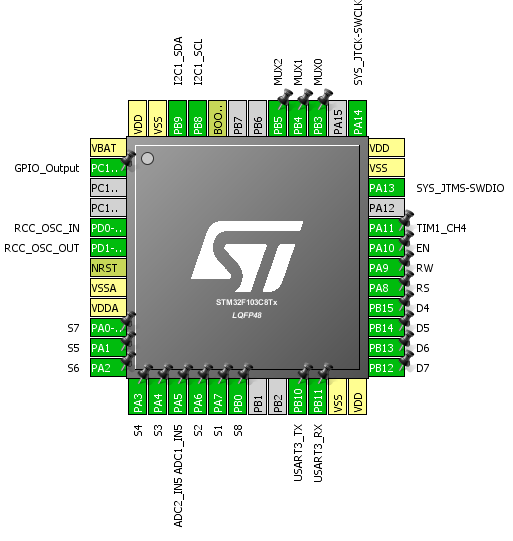
\includegraphics[scale=0.7]{imagens/pinagem_microcontrolador}
	\caption*{Fonte: Autoria Própria.}

\end{figure}

Como o microcontrolador proposto para este trabalho possui uma frequência de \textit{clock} maior que aquele utilizado por \citeonline{RUANI}, foi necessário descobrir a frequência de \textit{clock} ideal para alimentar as bobinas geradoras. Utilizando um \textit{software} chamado STM32Studio, pelo qual é possível monitorar variáveis em tempo real pelo computador, foi monitorada uma bobina sensora para alcançar o seu valor máximo quando o mais próximo possível da bobina geradora. Para isso, foi feito um pequeno teste com cada par sensor/gerador variando a frequência na bobina geradora de 95 $kHz$ até 105 $kHz$. Ao obter o valor máximo, este valor de frequência é deixado fixo para esse par.

\begin{figure}[H]
	\vspace{4mm}
	\centering
	\caption{Fluxograma que detalha a rotina desenvolvida para calibrar os sensores indutivos}
	\label{fig:fluxograma_calibragem_ind}
	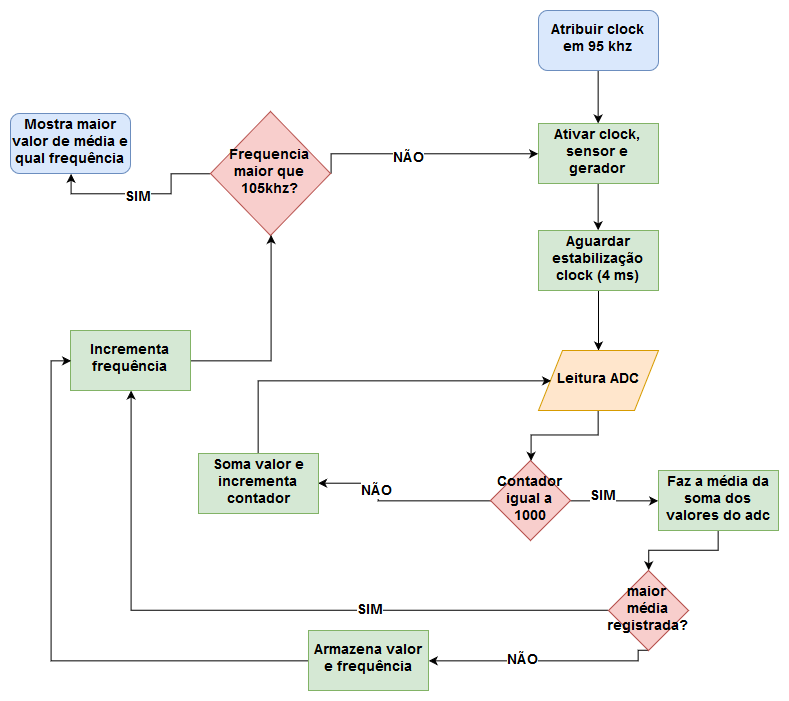
\includegraphics[scale=0.5]{imagens/calibrarIndutivo}	
	\caption*{Fonte: Autoria Própria.}
\end{figure}

Após configurados os valores para cada par sensor/gerador, foi feito o gesto que representa a letra A em LIBRAS, e o resultado obtido nos sensores indutivos pode ser observado no gráfico da Figura \ref{fig:sensores_letra_a}.

\begin{figure}[H]
	\vspace{4mm}
	\centering
	\caption{Valor dos sensores indutivos ao fazer o gesto da letra A em LIBRAS no software STM32Studio}
	\label{fig:sensores_letra_a}
	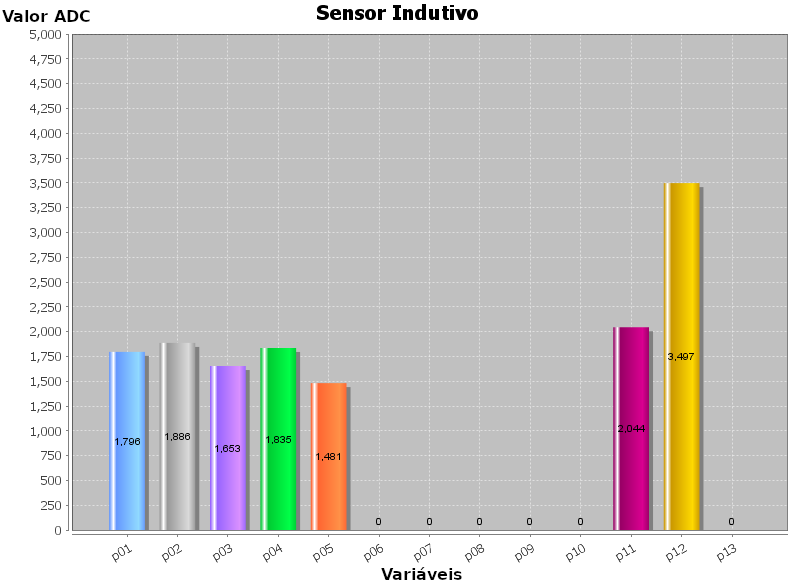
\includegraphics[scale=0.7]{imagens/LETRA_A_STMSTUDIO}
	\caption*{Fonte: Autoria Própria.}
\end{figure}

A relação de sensores e geradores com as variáveis exibidas na Figura \ref{fig:sensores_letra_a} é exibida na Tabela \ref{tab:relacao_sgv}.

\begin{table}[H]
	\vspace{4mm}
	\centering
	\caption{Relação de sensores e geradores com as variáveis da Figura \ref{fig:sensores_letra_a}}
	\label{tab:relacao_sgv}
	\resizebox{\textwidth}{!}{%
		\begin{tabular}{|l|l|l|l|l|l|l|l|l|l|l|l|l|l|}
			\hline
			\textbf{Variável} & p01 & p02 & p03 & p04 & p05 & p06 & p07 & p08 & p09 & p10 & p11 & p12 & p13 \\ \hline
			\textbf{Sensor} & S1 & S2 & S3 & S4 & S5 & S5 & S1 & S2 & S3 & S6 & G4 & G5 & G6 \\ \hline
			\textbf{Gerador} & G1 & G1 & G1 & G1 & G1 & G2 & G3 & G3 & G3 & G3 & S6 & S7 & S8 \\ \hline
		\end{tabular}%
	}
	\vspace{4mm}
	\caption*{Fonte: Autoria Própria.}
\end{table}

Na Figura \ref{tab:relacao_sgv} percebe-se que a medida p13 não está marcando um valor válido. Isso se deve ao fato do sensor/gerador terem dado defeito constantemente. Então foi analisada a necessidade deste sensor e foi decidido não utilizá-lo.
A rotina para a coleta dos dados de cada par sensor/gerador tem o funcionamento descrito pelo fluxograma da Figura \ref{fig:fluxograma_rotina_coleta}.
\begin{figure}[H]
	\vspace{4mm}
	\centering
	\caption{Fluxograma que detalha o funcionamento da rotina de coleta de dados do sensor indutivo.}
	\label{fig:fluxograma_rotina_coleta}
	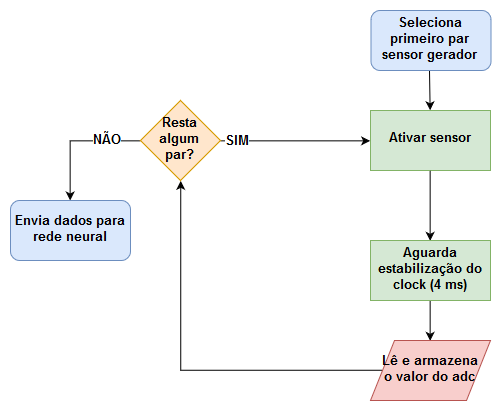
\includegraphics[scale=0.6]{imagens/rotinaColetaIndutivo}
	\caption*{Fonte: Autoria Própria.}
\end{figure}

A implementação da rotina de coleta de dados é exibida no Codigo \ref{cod:Indutivo}.

Após toda a codificação, foi testado o funcionamento com os mesmos valores da rede neural que foi implementada no trabalho anterior desenvolvido por \citeonline{RUANI}. Ao retirar um dos sensores indutivos, a entrada da rede neural implementada pelo \citeonline{RUANI} teria uma resposta errada, sendo. Considerando isto e também a diferença de periférico ADC do microcontrolador MSP430, utilizado no trabalho anterior, para o ADC do microcontrolador deste trabalho (STM32F103), foi decidido modificar a rede neural.

Porém, a resposta não estava satisfatória, devido a diferença dos periféricos A/D de um microcontrolador para outro. Então foi decidido refazer a rede neural.

O laço principal do \textit{firmware} é demonstrado no Código \ref{cod:mainloop}, onde é feita a coleta dos sensores indutivos, enviado para serial caso solicitado, e classificada a letra.

Para a implementação do \textit{display}, foi feito um código baseado na implementação de \cite{gihutDisplay}.

\subsection{Placa de adaptação para novo microcontrolador}
Para não refazer a placa toda, foi feita uma placa de adaptação para o novo microcontrolador, que possui como única função encaixar na placa de processamento de sinais e direcionar os pinos para os pinos corretos do stm32.

\begin{figure}[H]
	\vspace{4mm}
	\centering
	\caption{Vista das ligações da placa de adaptação para o microcontrolador stm32f103c8t6}
	\label{fig:placa2}
	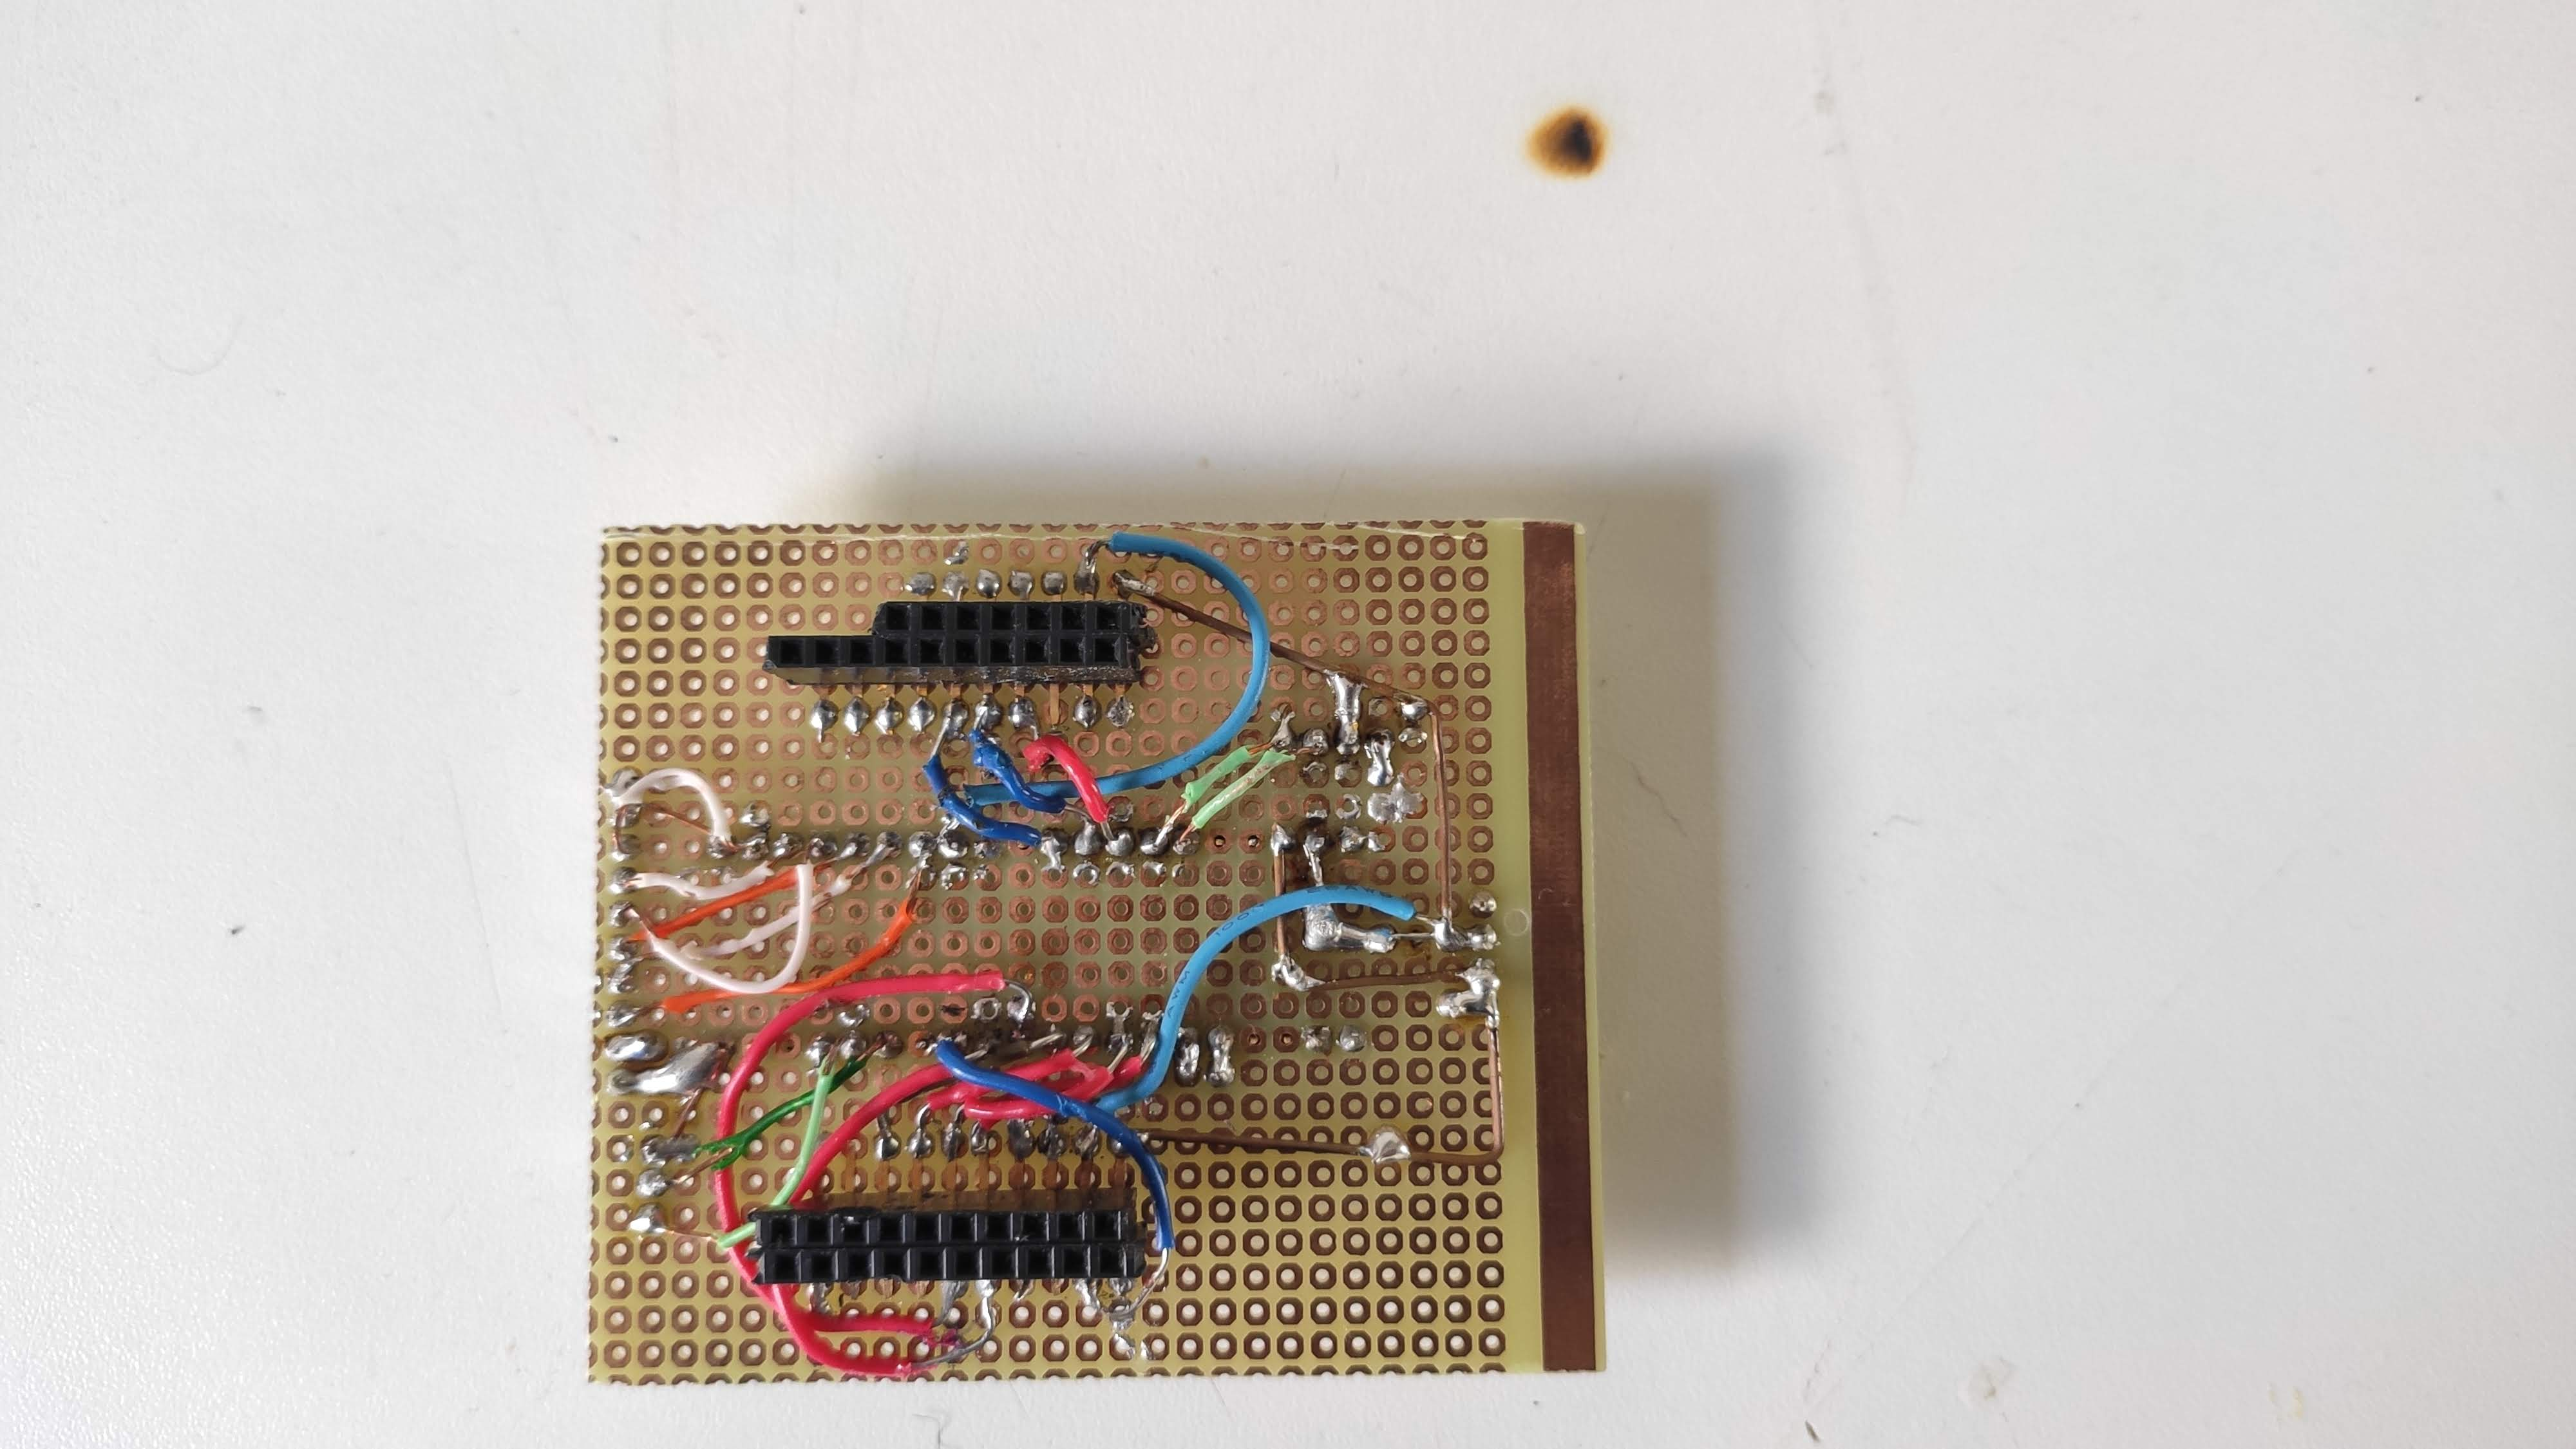
\includegraphics[scale=0.12, trim={20cm 2cm 45cm 15cm}, clip]{imagens/placa2}
	\caption*{Fonte: Autoria Própria.}
\end{figure}
Como demonstrado nas Figura \ref{fig:placa2}, a placa foi feita a partir de uma placa ilhada de contatos pela facilidade de fazer as ligações sem precisar de muito planejamento e software para produzi-la.

O posicionamento dos componentes da placa pode ser visto na Figura \ref{fig:placa1}. A placa conta com barras de pinos para ligar o \textit{display}, barra de pinos para conectar a interface serial e comunicar com o computador, barra de pinos para conectar o sensor inercial MPU6050, e também a barra de pinos para a alimentação das placas.

\begin{figure}[H]
	\vspace{4mm}
	\centering
	\caption{Vista de cima da placa de adaptação para o microcontrolador stm32f103c8t6}
	\label{fig:placa1}
	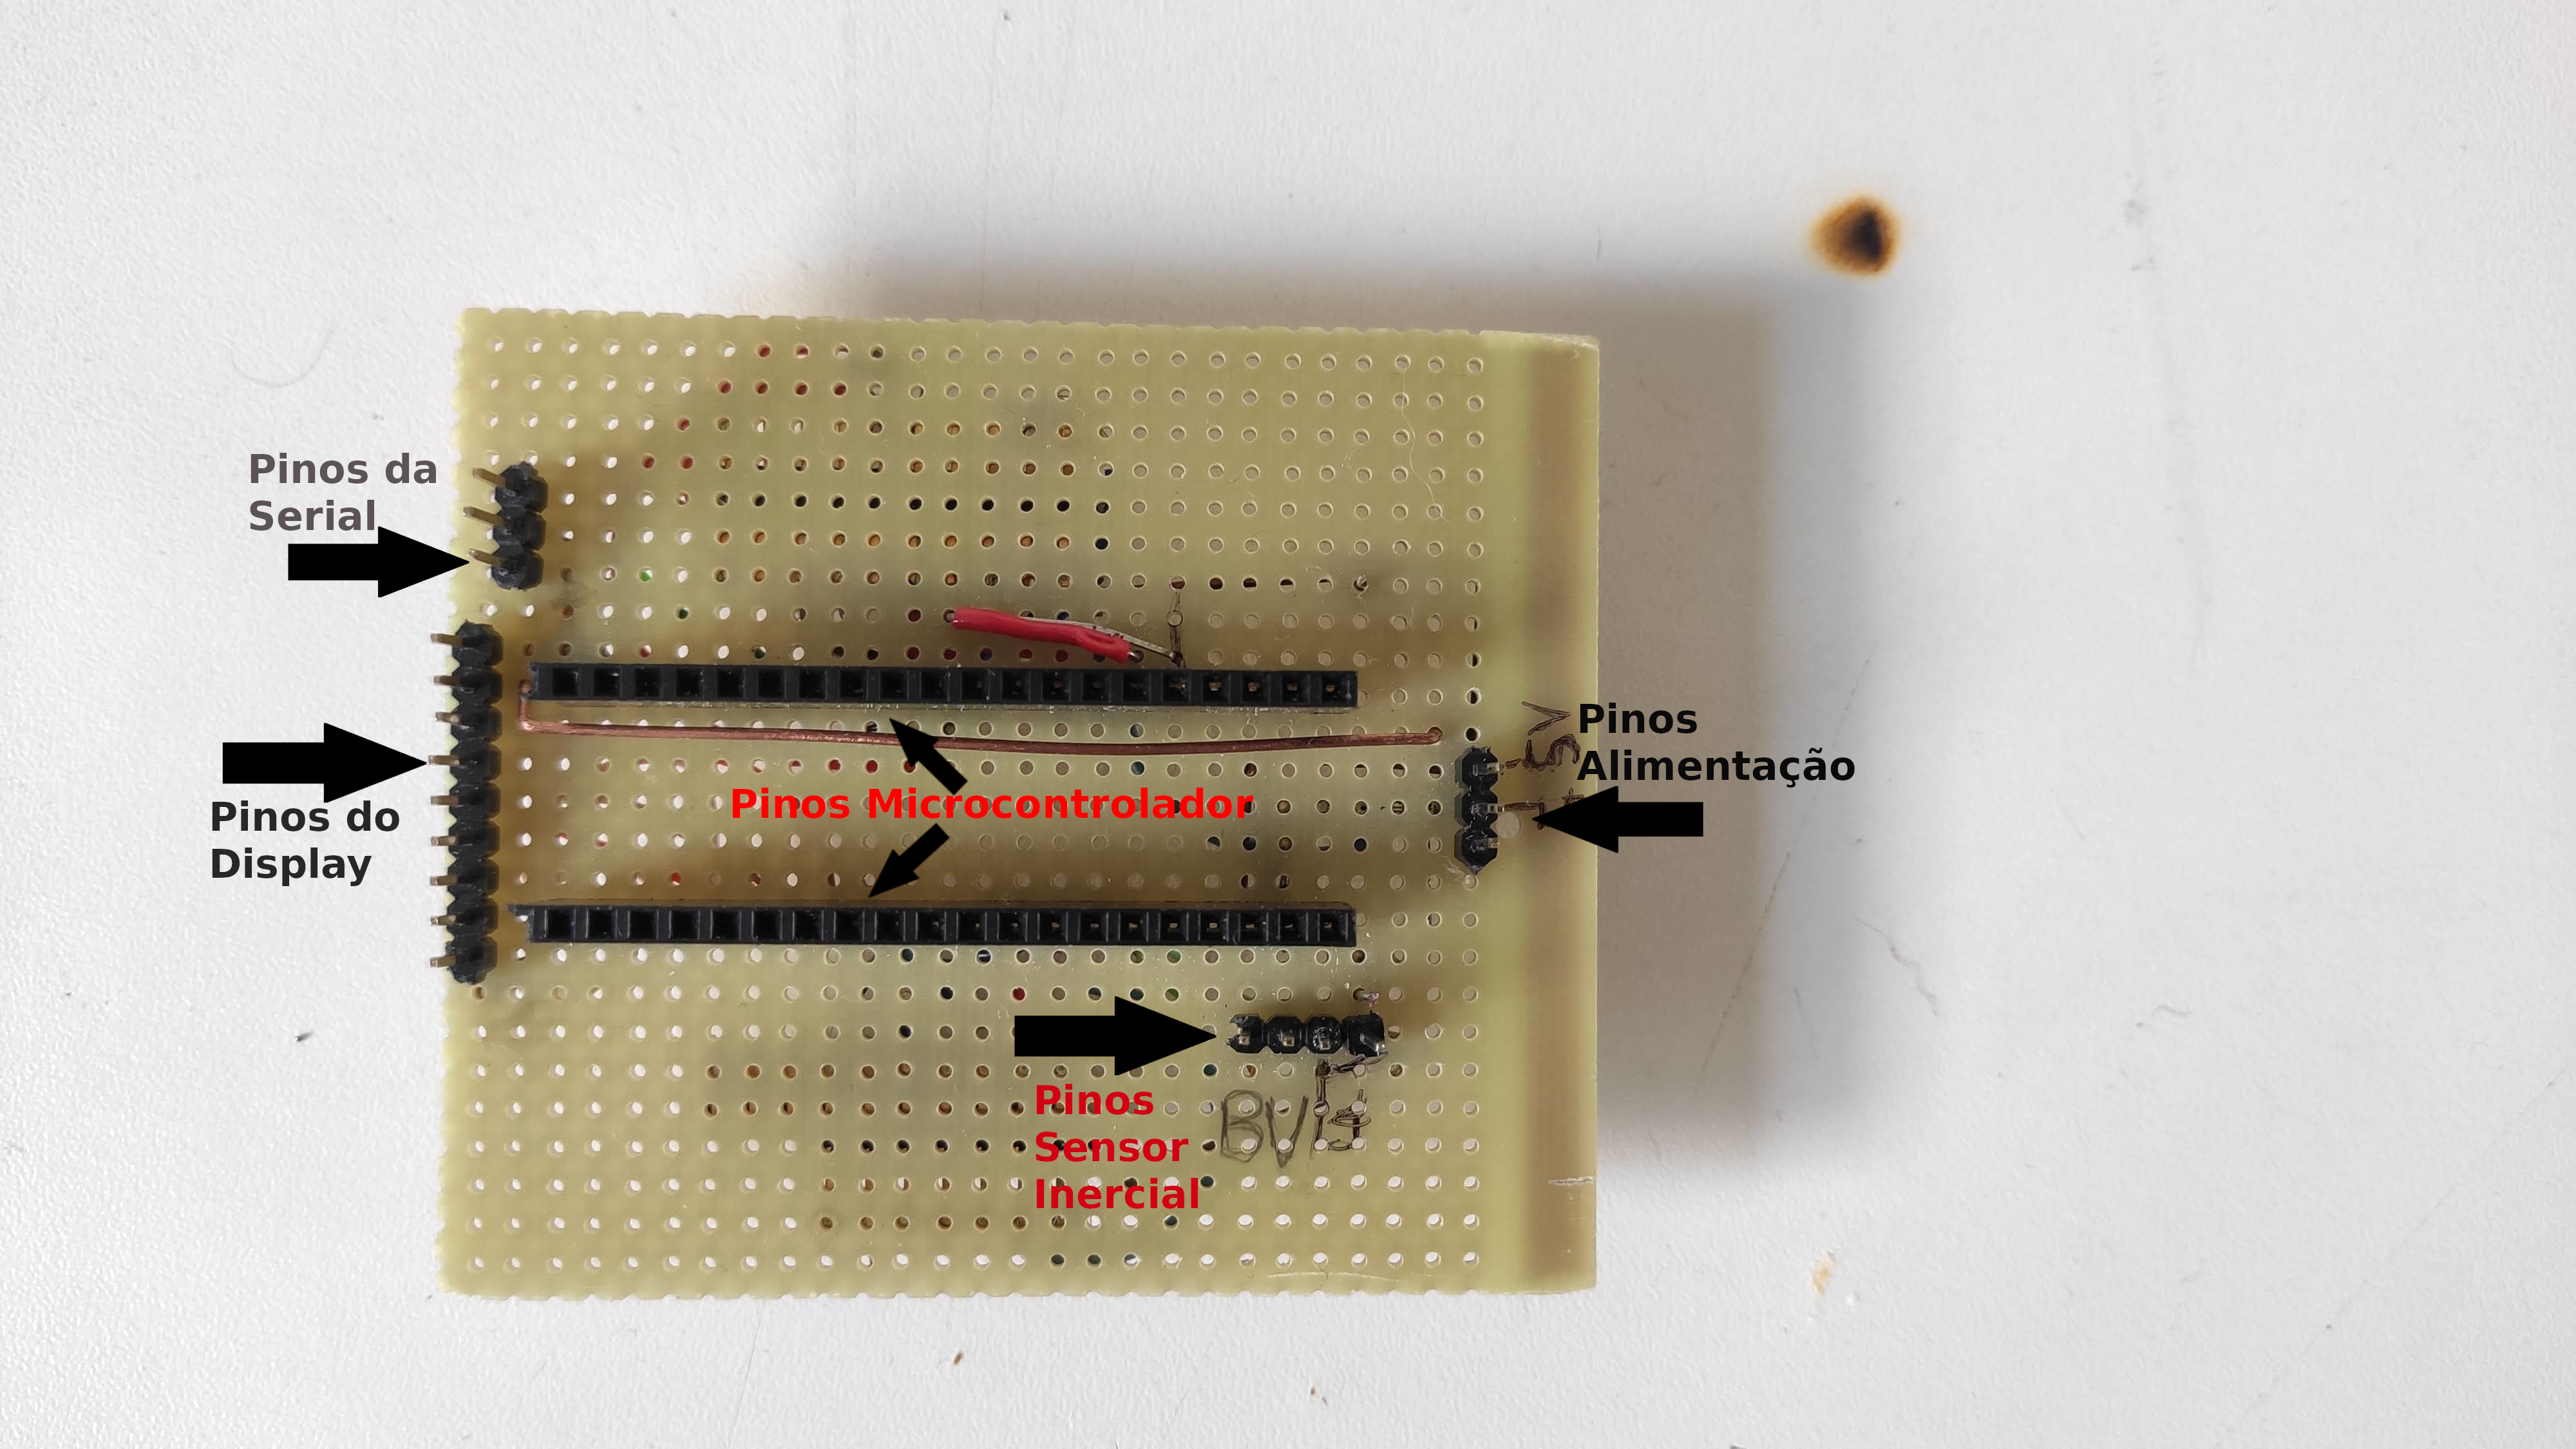
\includegraphics[scale=0.5, trim={2.5cm 3cm 8cm 4cm}, clip]{imagens/placa1}	
	\caption*{Fonte: Autoria Própria.}
\end{figure}

\subsection{Configuração sensor MPU6050 e Processamento de sinais}
Está sessão detalha a configuração do sensor MPU6050 e explica como foi feita o processamento dos sinais vindos do sensor. 	
\subsubsection{Configuração e calibração do sensor MPU-6050}
O sensor inercial, utilizando comunicação de circuitos inter-integrados ou I²C, sendo necessário o uso e configuração de uma interface serial neste padrão no microcontrolador.

 A biblioteca de abstração de hardware (HAL) disponibilizada pela fabricante do microcontrolador facilita a configuração de periféricos, necessitando apenas de poucas funções para configurar. Utilizando o \textit{datasheet} do sensor MPU6050, foi identificada a sequência de passos para iniciar, calibrar e ler os valores. Para calibrar o acelerômetro, são estimados os valores de \textit{offsets} necessários para o funcionamento do sensor. Esses valores variam para cada placa fabricada. Então foi desenvolvida uma rotina de calibração para o sensor. O sensor deve ser posicionado em uma superfície plana com o eixo Z em 90 graus com a superfície, como é exibido na Figura \ref{fig:MPU_Calb}.

\begin{figure}[H]
	\vspace{4mm}
	\centering
	\caption{Posicionamento da MPU6050 e seus eixos para a calibração}
	\label{fig:MPU_Calb}
	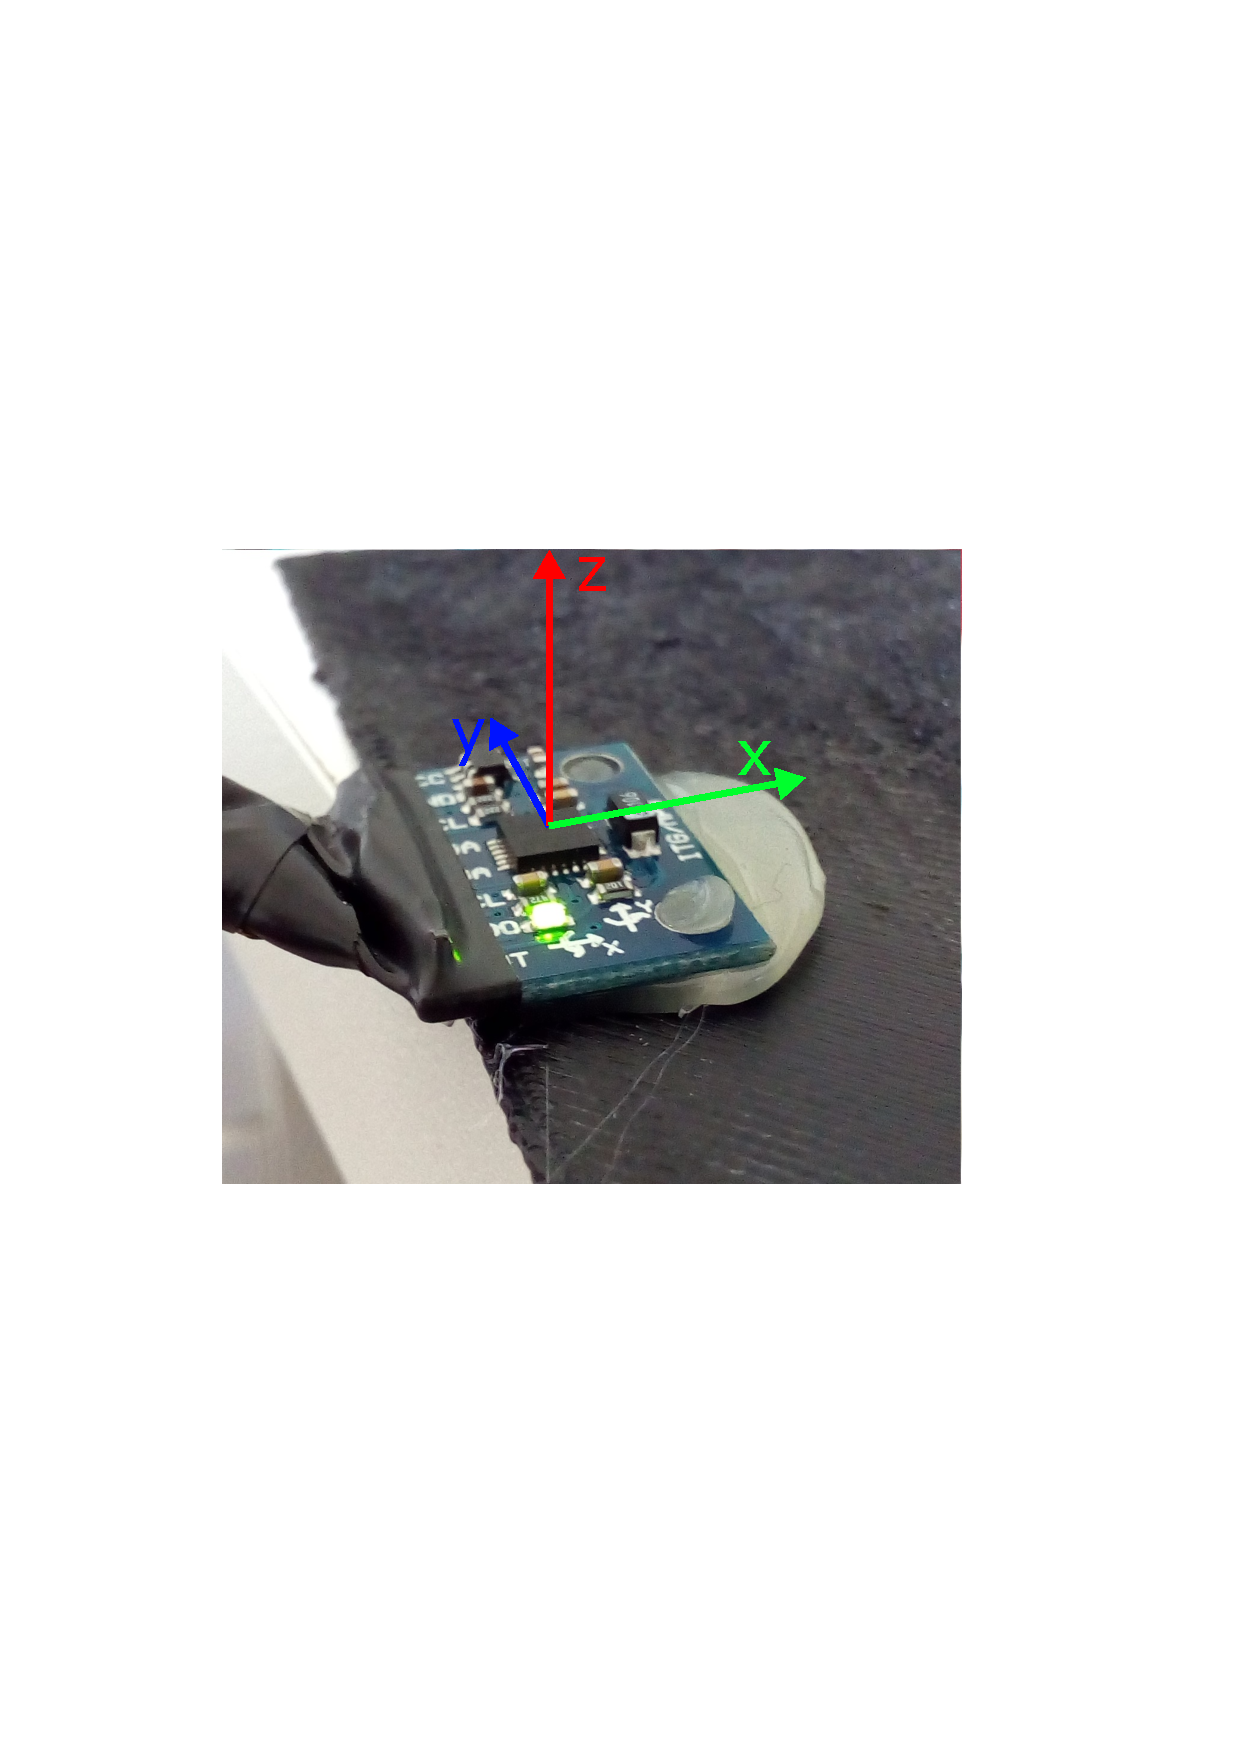
\includegraphics[scale=0.7, trim={5cm 10cm 7cm 9.3cm}, clip]{imagens/mpu_calib.pdf}
	\caption*{Fonte: Autoria Própria.}
\end{figure}

Para este trabalho, foi utilizado somente o acelerômetro para a detecção dos movimentos.

\subsubsection{Letras conflitantes e processamento dos sinais}
Observando todas as letras do alfabeto de LIBRAS (Figura \ref{fig:alfabeto}), nota-se que algumas letras tem o mesmo posicionamento de mãos, sendo apenas diferenciadas pelo movimento. Essas são: J e I; P, K e H; e X e Z; No trabalho anterior desenvolvido por \citeonline{RUANI}, foram deixadas de fora as letras com movimento (X, K, H, e J). Para reconhecer todas as letras, foi utilizado o acelerômetro para detecção de movimento.
Ao incluir detecção de movimento, as letras que contém a mesma posição de mão, como as letras J e I, tornam-se conflitantes, mesmo que a letra I não contenha movimento, porque a posição de mão dela é igual ao da letra J. O mesmo ocorre com as letras P, K, e H, onde a letra P não contém movimento e as letras H e K usam movimento.

 O trabalho do acelerômetro do sensor inercial é detectar esse movimento ocorrido. Na Figura \ref{fig:letrasMov}, são exibidas apenas as letras com movimentação. Posicionando o eixos de coordenadas do sensor inercial na luva como demonstrado na Figura \ref{fig:LuvaMPU}.

\begin{figure}[H]
	\vspace{4mm}
	\centering
	\caption{Posicionamento do sensor inercial na luva com eixo de coordenadas.}
	\label{fig:LuvaMPU}
	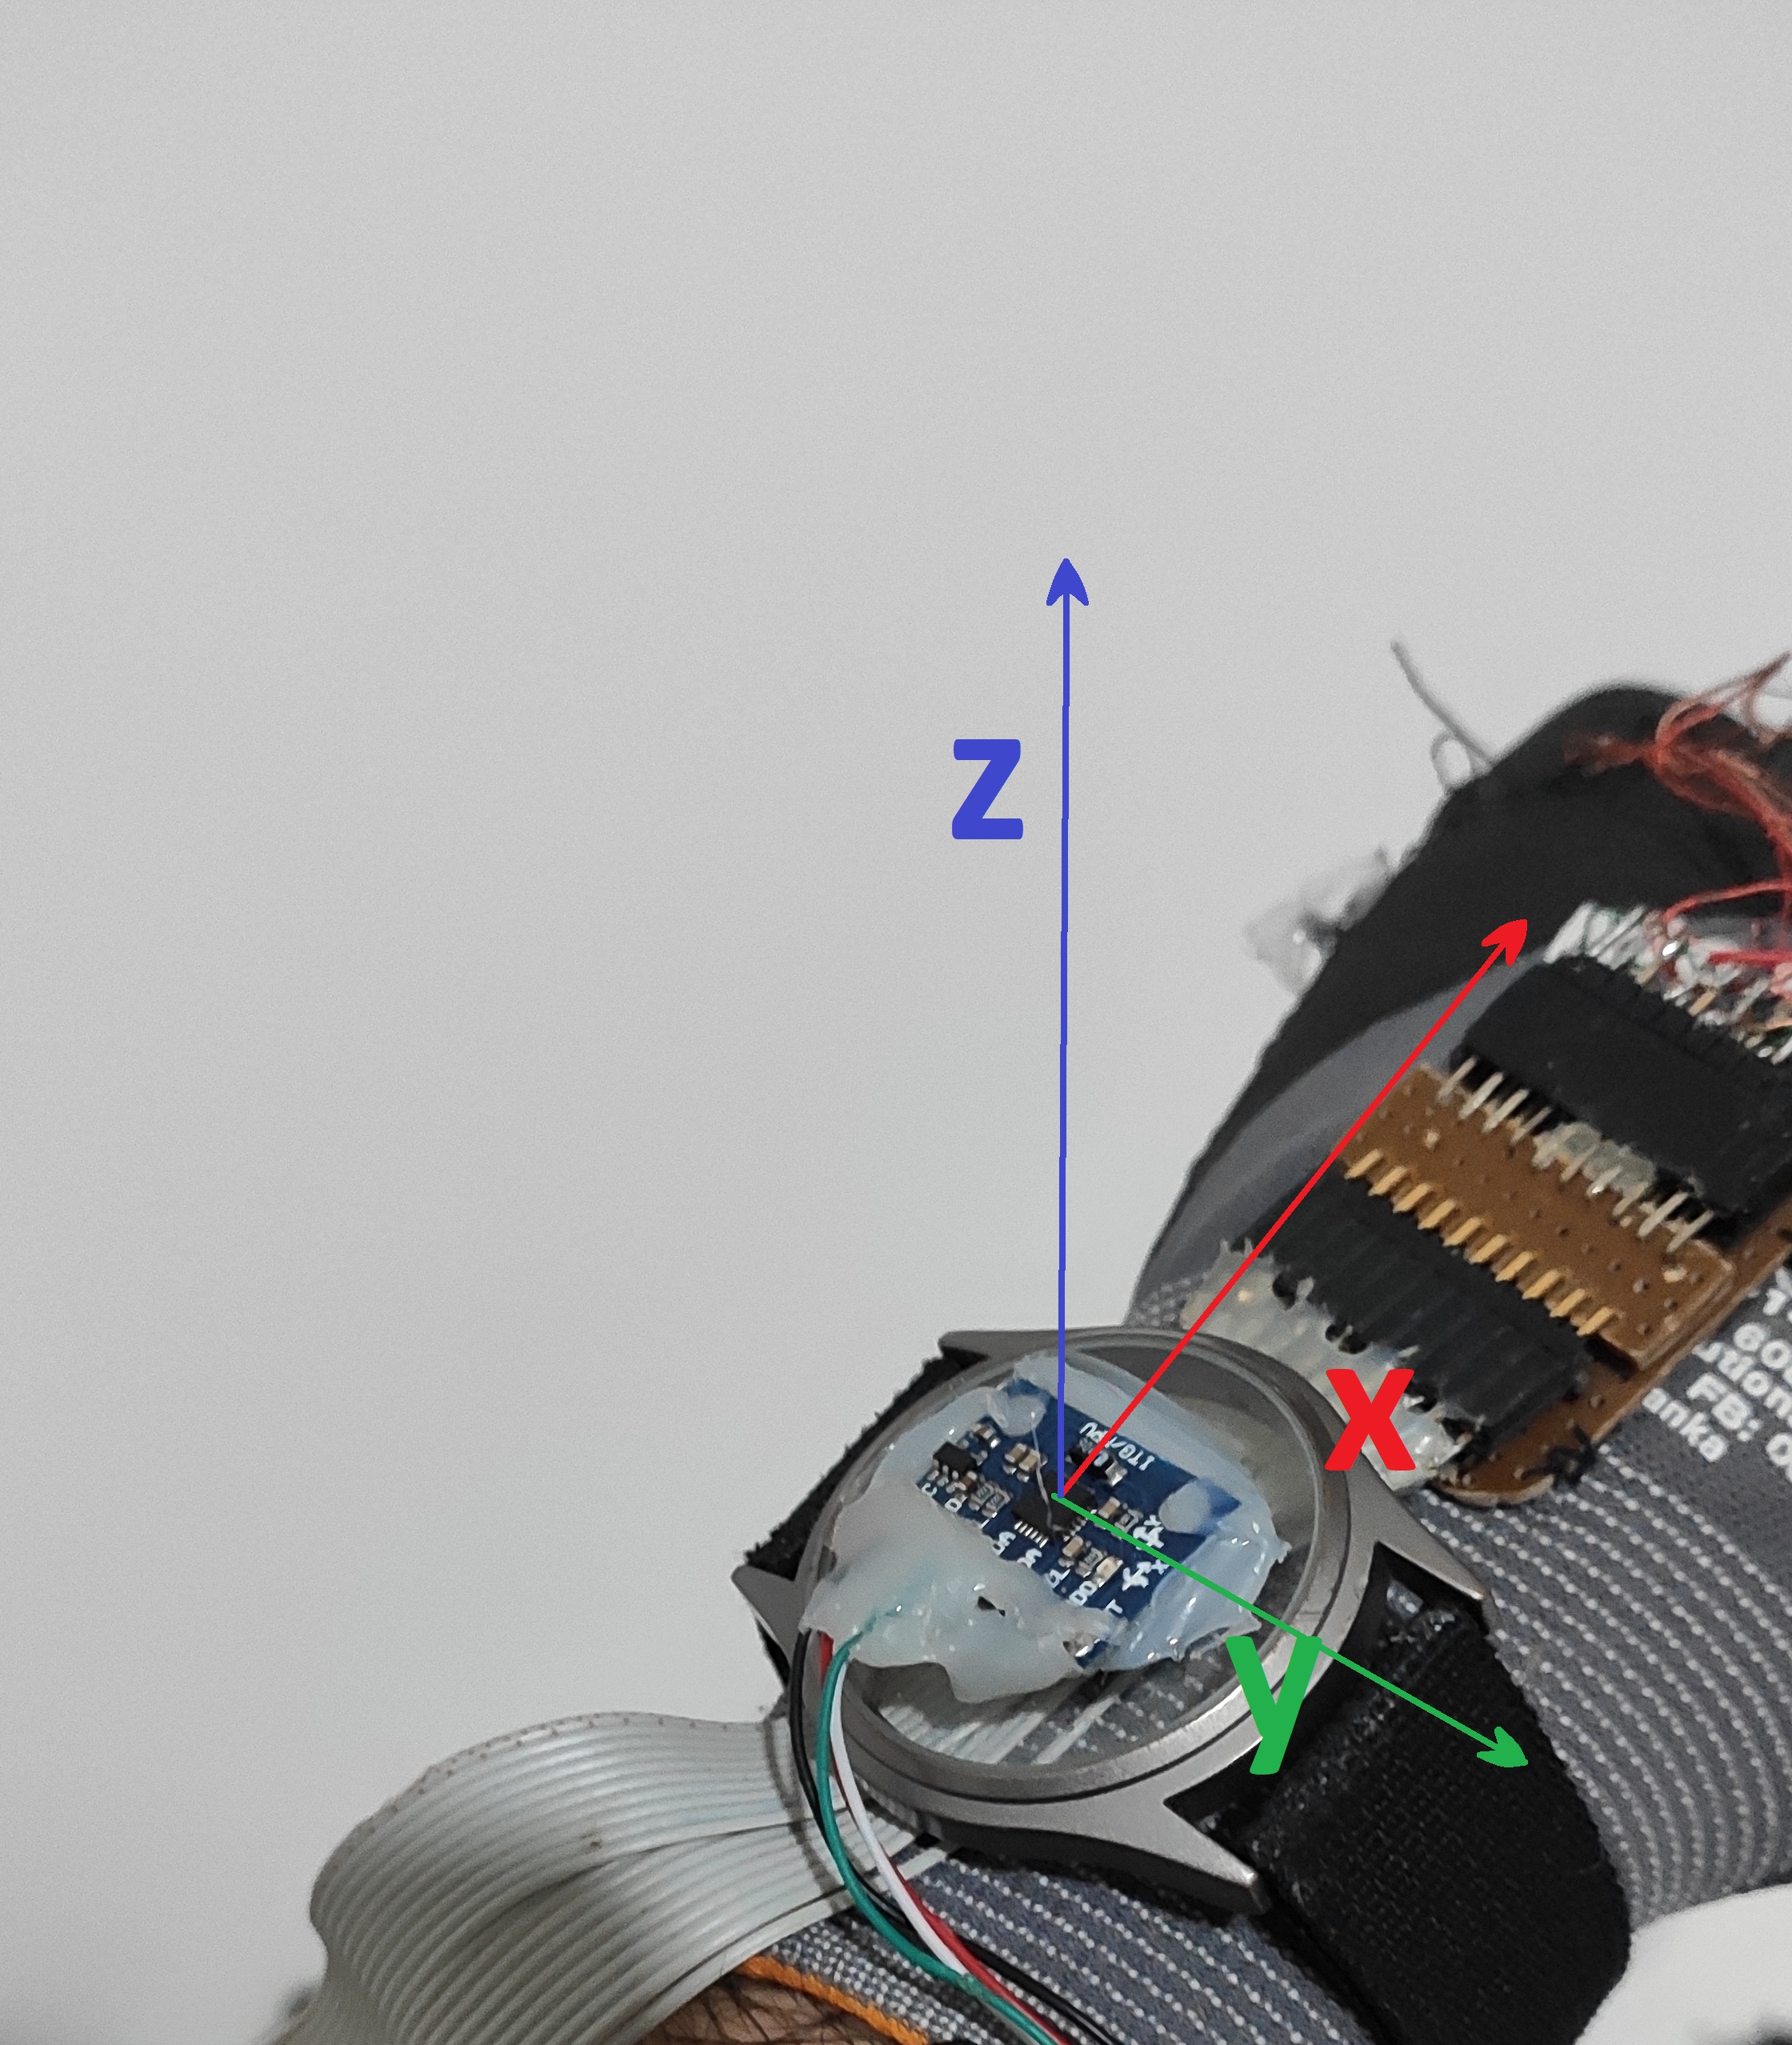
\includegraphics[scale=0.1]{imagens/luvaComMput}
	\caption*{Fonte: Autoria Própria.}
\end{figure}

Para detectar os movimentos das letra exibidas na Figura \ref{fig:letrasMov}, foram utilizadas as 3 coordenadas do acelerômetro ($x, y,$ e $z$), e a coordenada de rotação Roll.

\begin{figure}[H]
	\vspace{4mm}
	\centering
	\caption{Letras do alfabeto de libras que contém movimento.}
	\label{fig:letrasMov}
	
\includegraphics[scale=0.2]{imagens/letras_movimento}	
	\caption*{Fonte: Autoria Própria.}
\end{figure}

Os sinais provenientes da luva são os doze pares sensor/gerador. O sinal lido das bobinas pelo ADC já está processado, somente necessitando normalizar. E também os sinais vindos do acelerômetro.

Para captar o movimento, foi definido uma janela de tempo de $500$ $ms$, que é o tempo necessário para fazer o movimento de uma letra. Na Figura \ref{fig:espec_ACC} pode ser visto os sinais do acelerômetro no período de $500$ $ms$.

\begin{figure}[H]
	\vspace{4mm}
	\centering
	\caption{Gráficos dos sinais do acelerômetro, amostrando $500$ $ms$.}
	\label{fig:espec_ACC}
	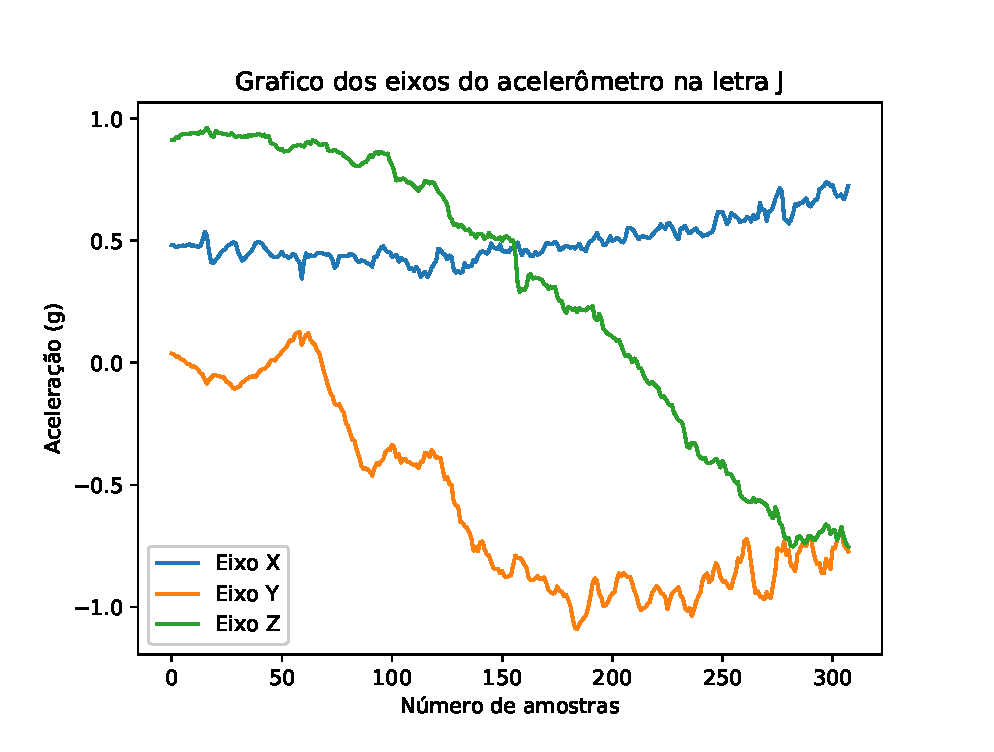
\includegraphics[scale=0.45]{imagens/espectro_acc.eps}
	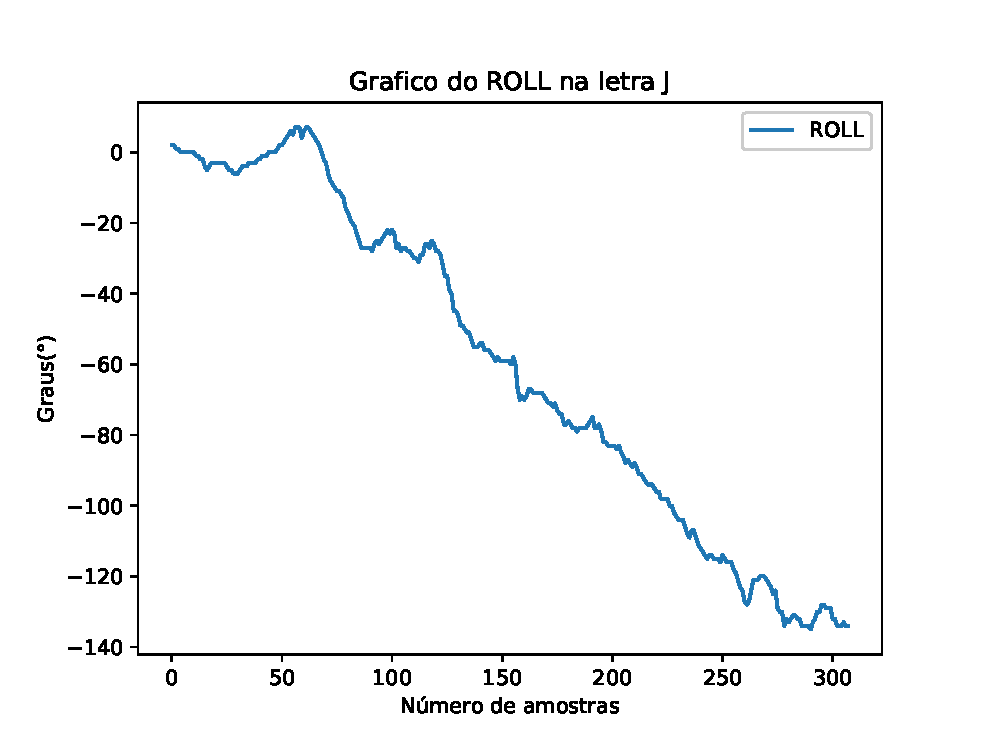
\includegraphics[scale=0.45]{imagens/roll_acc.eps}	
	\caption*{Fonte: Autoria Própria.}
\end{figure}

Essa janela de tempo é dividida em 10 pedaços, e a cada $50$ $ms$, são coletados os dados dos eixos do sensor inercial, e sempre a amostra mais velha dos dados é descartada, fazendo com que a janela de $500$ $ms$ deslize no tempo. Um exemplo de como será a janela pode ser visto na Figura \ref{fig:janela}.

\begin{figure}[H]
	\vspace{4mm}
	\centering
	\caption{Janela de amostras}
	\label{fig:janela}
	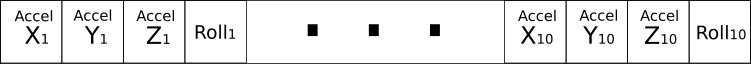
\includegraphics[scale=0.7]{imagens/janela.png}
	\caption*{Fonte: Autoria Própria.}
\end{figure}

\subsection{Redes Neurais Implementadas}

Para manter o foco na solução sugerida por este trabalho, foram separadas as letras em dois grupos: letras sem conflito, e as letras conflitantes.
As letras sem conflito são aquelas que somente o sensor indutivo consegue classificar, sem a necessidade do sensor inercial. E as letras conflitantes são as quais tem a necessidade de utilizar o sensor inercial como diferencial entre elas. As letras consideradas conflitantes são P, H, K, I, J, Z, X.
Considerando esses dois grupos, foram feitas duas redes neurais. A posição de mão das letras conflitantes entram na classificação das não conflitantes, mas só é exibido um resultado quando é executada a segunda classificação com os dados do sensor inercial.

\subsubsection{Rede Neural para os sensores indutivos}
Como já mencionado na subseção \ref{sec:transf}, a rede neural que trata dos sinais provenientes dos sensores indutivos (pares de bobinas sensora/geradora) foi refeita, ao retirar um dos sensores indutivos, uma das entradas sempre será zero afetando o desempenho do sistema.

As características são bem definidas como sendo cada par de bobinas sensora/geradora da luva. Foi criada um Perceptron Multi Camada (MLP) com 21 neurônios de camada oculta, utilizando a função de ativação tangente hiperbólica (Sessão \ref{sec:funcao}). 

O treinamento foi feito com um conjunto de 50 amostras de cada letra, onde 75\% para treinamento e 25\% para teste da rede. Esse processo de divisão dos dados é feito com uma mistura na ordem dos dados. Para permanecer parecida com a rede implementada no trabalho anterior, foi utilizada a mesma quantia de neurônios de camada oculta (21 neurônios).

O código \ref{cod:rede1} foi elaborado para o treinamento, obtendo uma taxa de acerto de 96,36\% ao final do treinamento e teste. \hspace{20pt}

Os dados dos sensores de cada letra feita foi armazenada em arquivos, e a função arruma\_dados é responsável por juntar esses dados em uma matriz de características. Após as características são redimensionadas para ficar no intervalo da função de ativação de $[-1, 1]$. Após isso é feita a divisão dos dados em vetores de teste e treino, (x\_train e x\_test). Então é feito o treino chamando a função \textit{fit} do \textit{MLPClassifier}. O resultado da classificação é visualizado com a função \textit{predict}, na qual usa o vetores de teste para comparar a classificação feita pela rede e a resposta real.

Para efetivamente fazer a classificação, é implementado o método \textit{feedfoward}, utilizando os pesos obtidos no treinamento. Resultando no Código \ref{cod:feedforward1}.

Após a classificação, para transformar o número em uma letra é utilizada uma função de pós-processamento descrita no Código \ref{cod:pos1}.

Nas letras de retorno pode-se notar os números 1, 2, e 3. Essas são as classes de pose de mão que são das letras conflitantes, esse é a ligação com a outra rede neural implementada, ou seja, não são exibidos esses números no \textit{display}.

\subsubsection{Rede Neural sensor inercial}
Considerando os dados já processados, foram colhidos pela serial e inseridos no código em Python para treinamento da rede. As características
são elas que são 10 pedaços de tempo em que cada pedaço tem 4 valores. Foram colhidos 25 amostras de cada movimento, incluindo uma posição sem movimento. No Código \ref{cod:rede2}, está demonstrado o treinamento da rede responsável pelo acelerômetro. Foi utilizado a função de ativação tangente hiperbólica. Utilizando 80 \% dos dados para treino e 20 \% para teste separados aleatoriamente.
 
 
A função \textit{LoadFromCsv} carrega os amostras dos arquivos e reúne em um vetor de características. Então esses dados são redimensionados para se adequar a função de ativação que é o intervalo de $[-1, 1]$. Então são separados os conjuntos de treino e teste para executar a função \textit{fit} que treina a rede neural. A função \textit{predict} compara os valores reais de classificação com os valores classificados e retorna o valor de acerto da rede treinada.

A função de \textit{feedfoward} implementada é a mesma do Código \ref{cod:feedforward1}, mudando apenas o pesos. O pós-processamento também só alterando o vetor de classes de saída que são as do Código \ref{cod:feedfor2}.

A função que faz a ligação das duas redes neurais é descrita no Código \ref{cod:classify}, onde são os dados do sensor indutivo são tratados e classificados. Caso a classificação seja uma das classes das letras conflitantes (1, 2, ou 3), então é acionado o acelerômetro para detectar o movimento e depois ele é classificado. No diagrama da Figura \ref{fig:fluxograma_trabalho_todo} está o detalhado o \textit{firmware} desenvolvido.
\begin{figure}[H]
	\centering
	\caption{Fluxograma que descreve o comportamento do \textit{firmware} a ser desenvolvido.}
	\label{fig:fluxograma_trabalho_todo}
	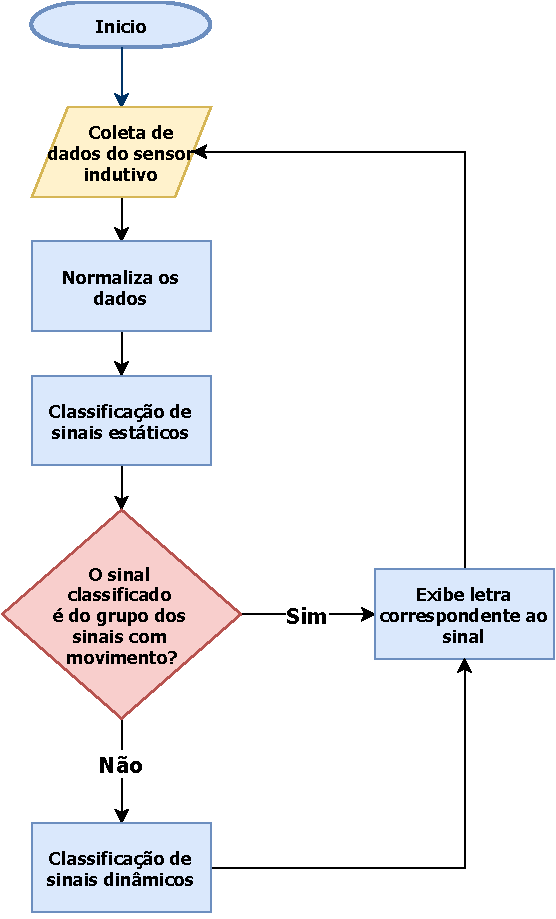
\includegraphics[scale=0.8]{imagens/fluxograma_trabalho_todo.pdf}	
	\caption*{Fonte: Autoria Própria.}
\end{figure}
\chapter{Resultados}
Neste capítulo são demonstrados os resultados obtidos após o desenvolvimento do projeto.
\section{Sistema completo}

 O sistema completado é demonstrado na Figura \ref{fig:luvaMontada}.

\begin{figure}[H]
	\centering
	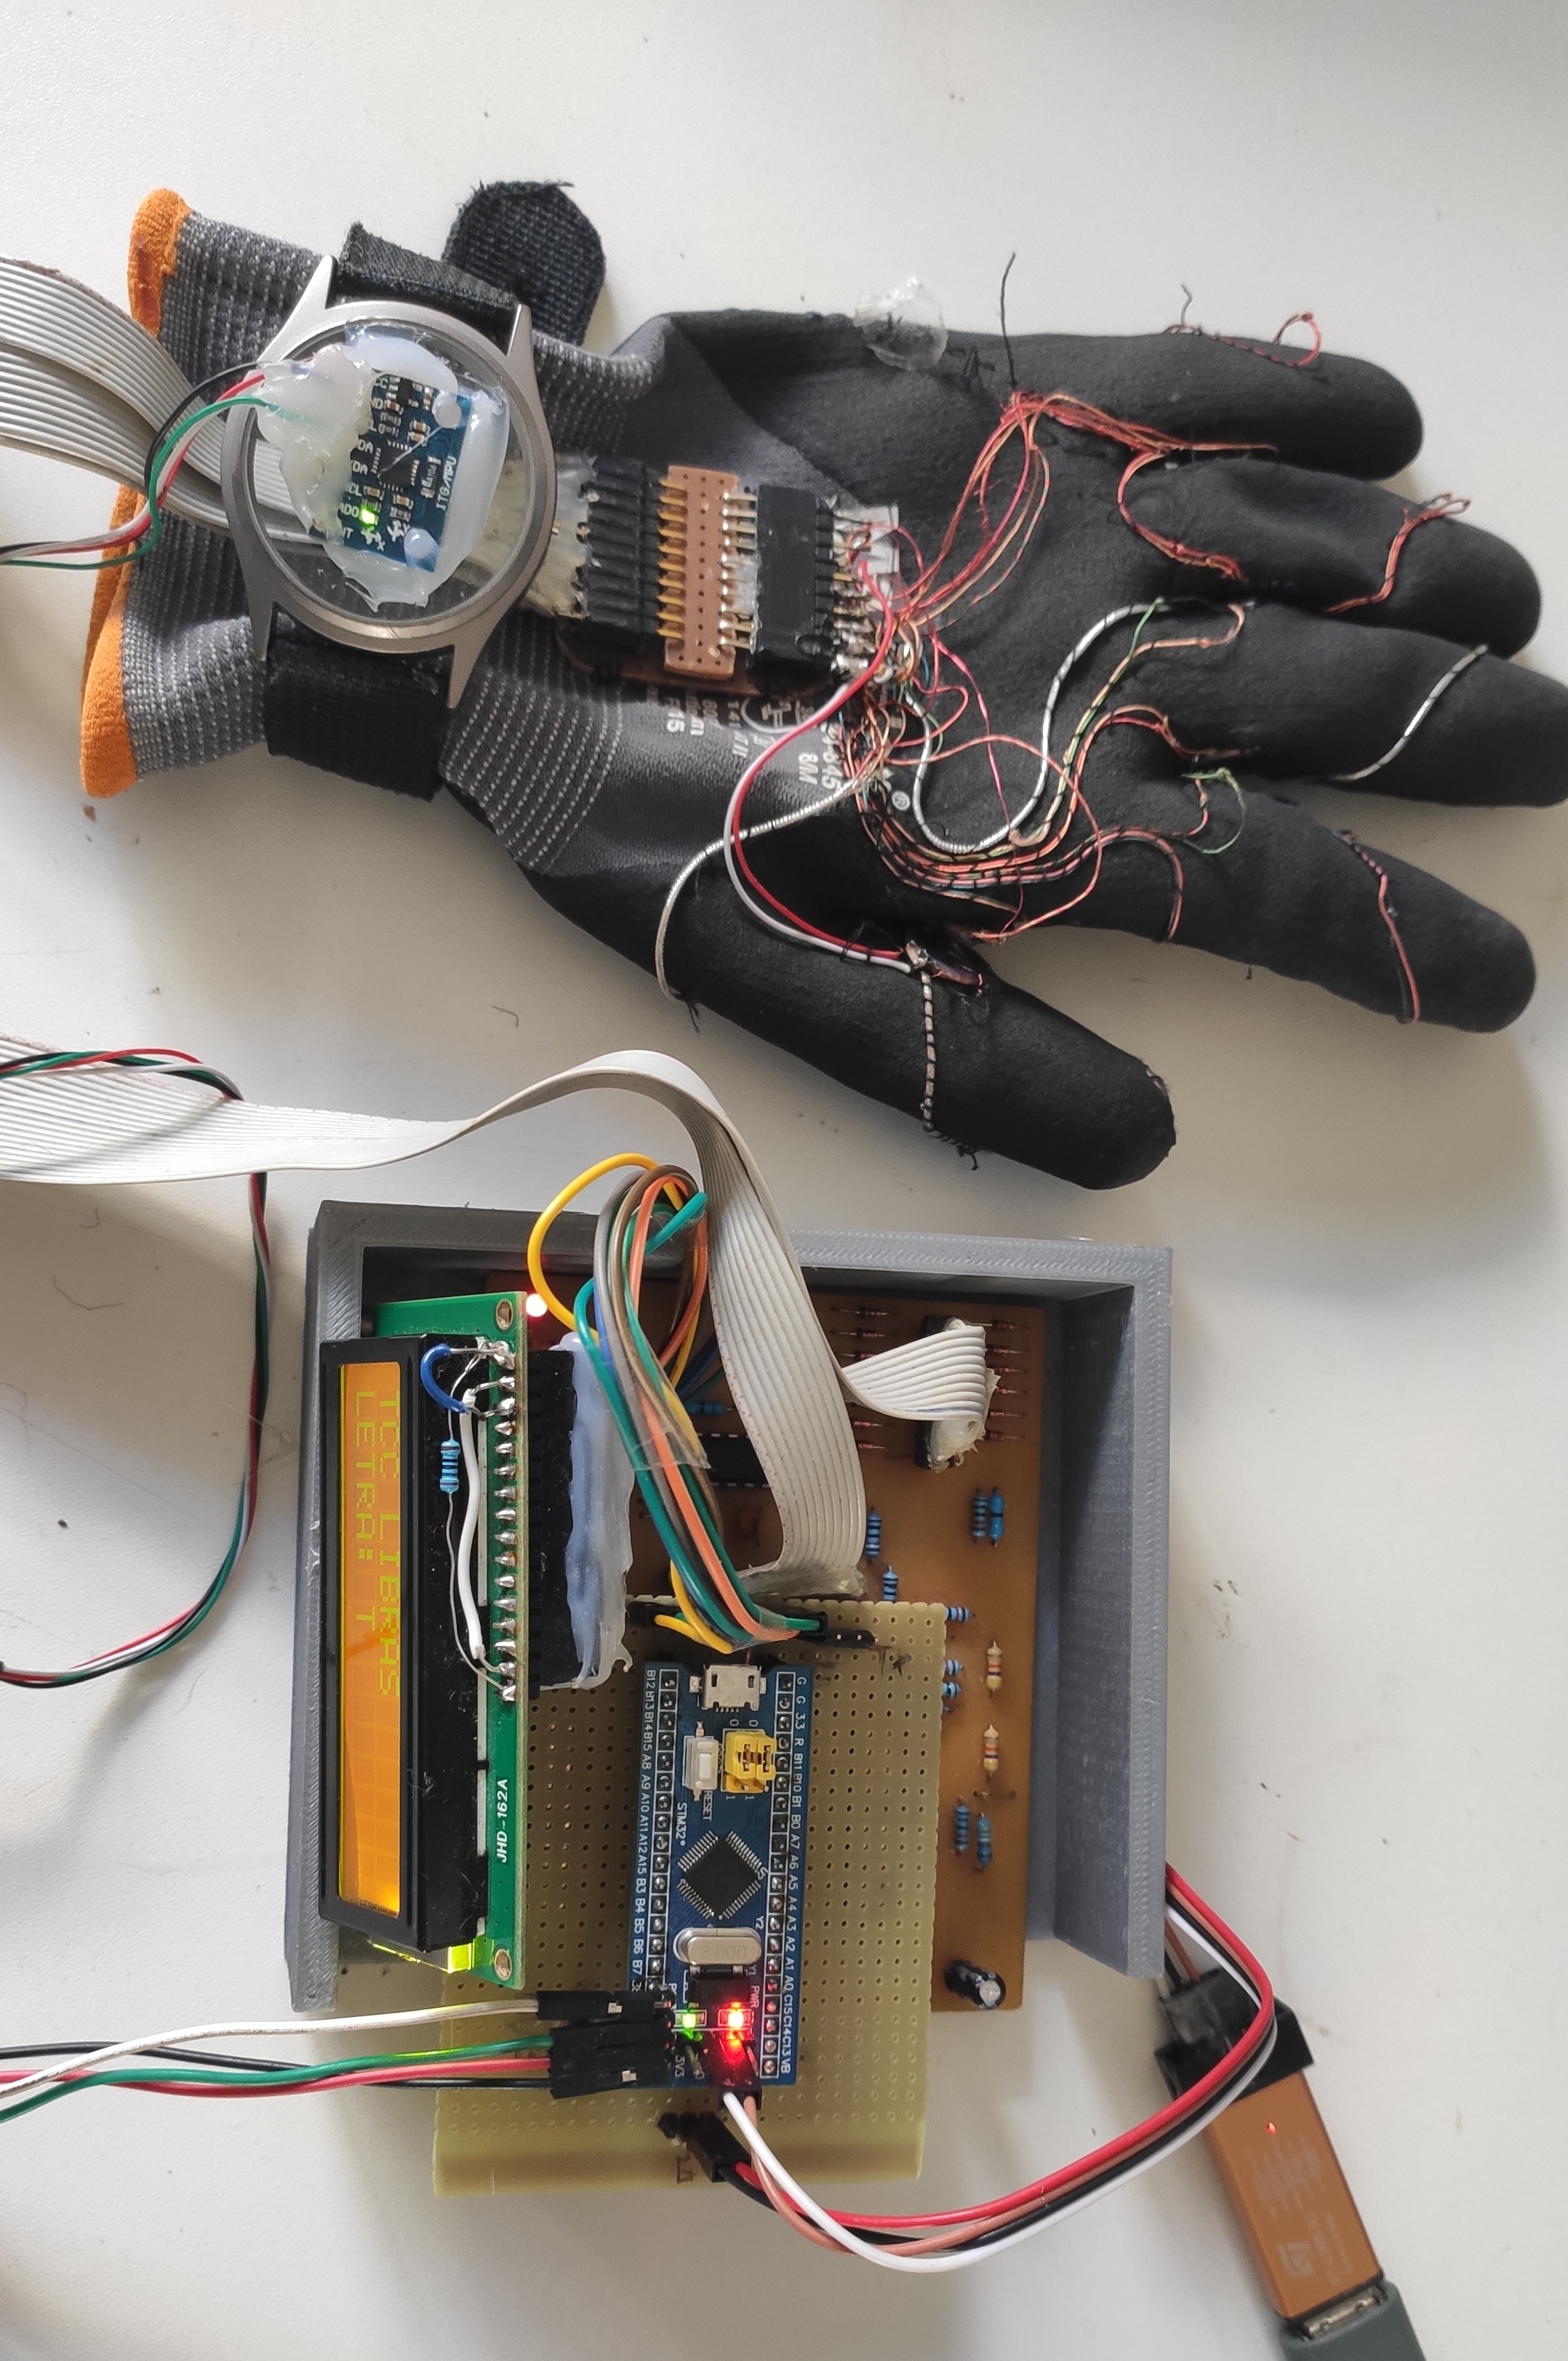
\includegraphics[scale=0.1]{imagens/conjuntoFinal.jpg}
	\caption{Conjunto ao final do trabalho.}
	\label{fig:luvaMontada}
\end{figure}

A Figura \ref{fig:letraC} apresenta uma demonstração da luva formando a letra C e também o \textit{display} mostrando a classificação correta da letra.

\begin{figure}[H]
	\centering
	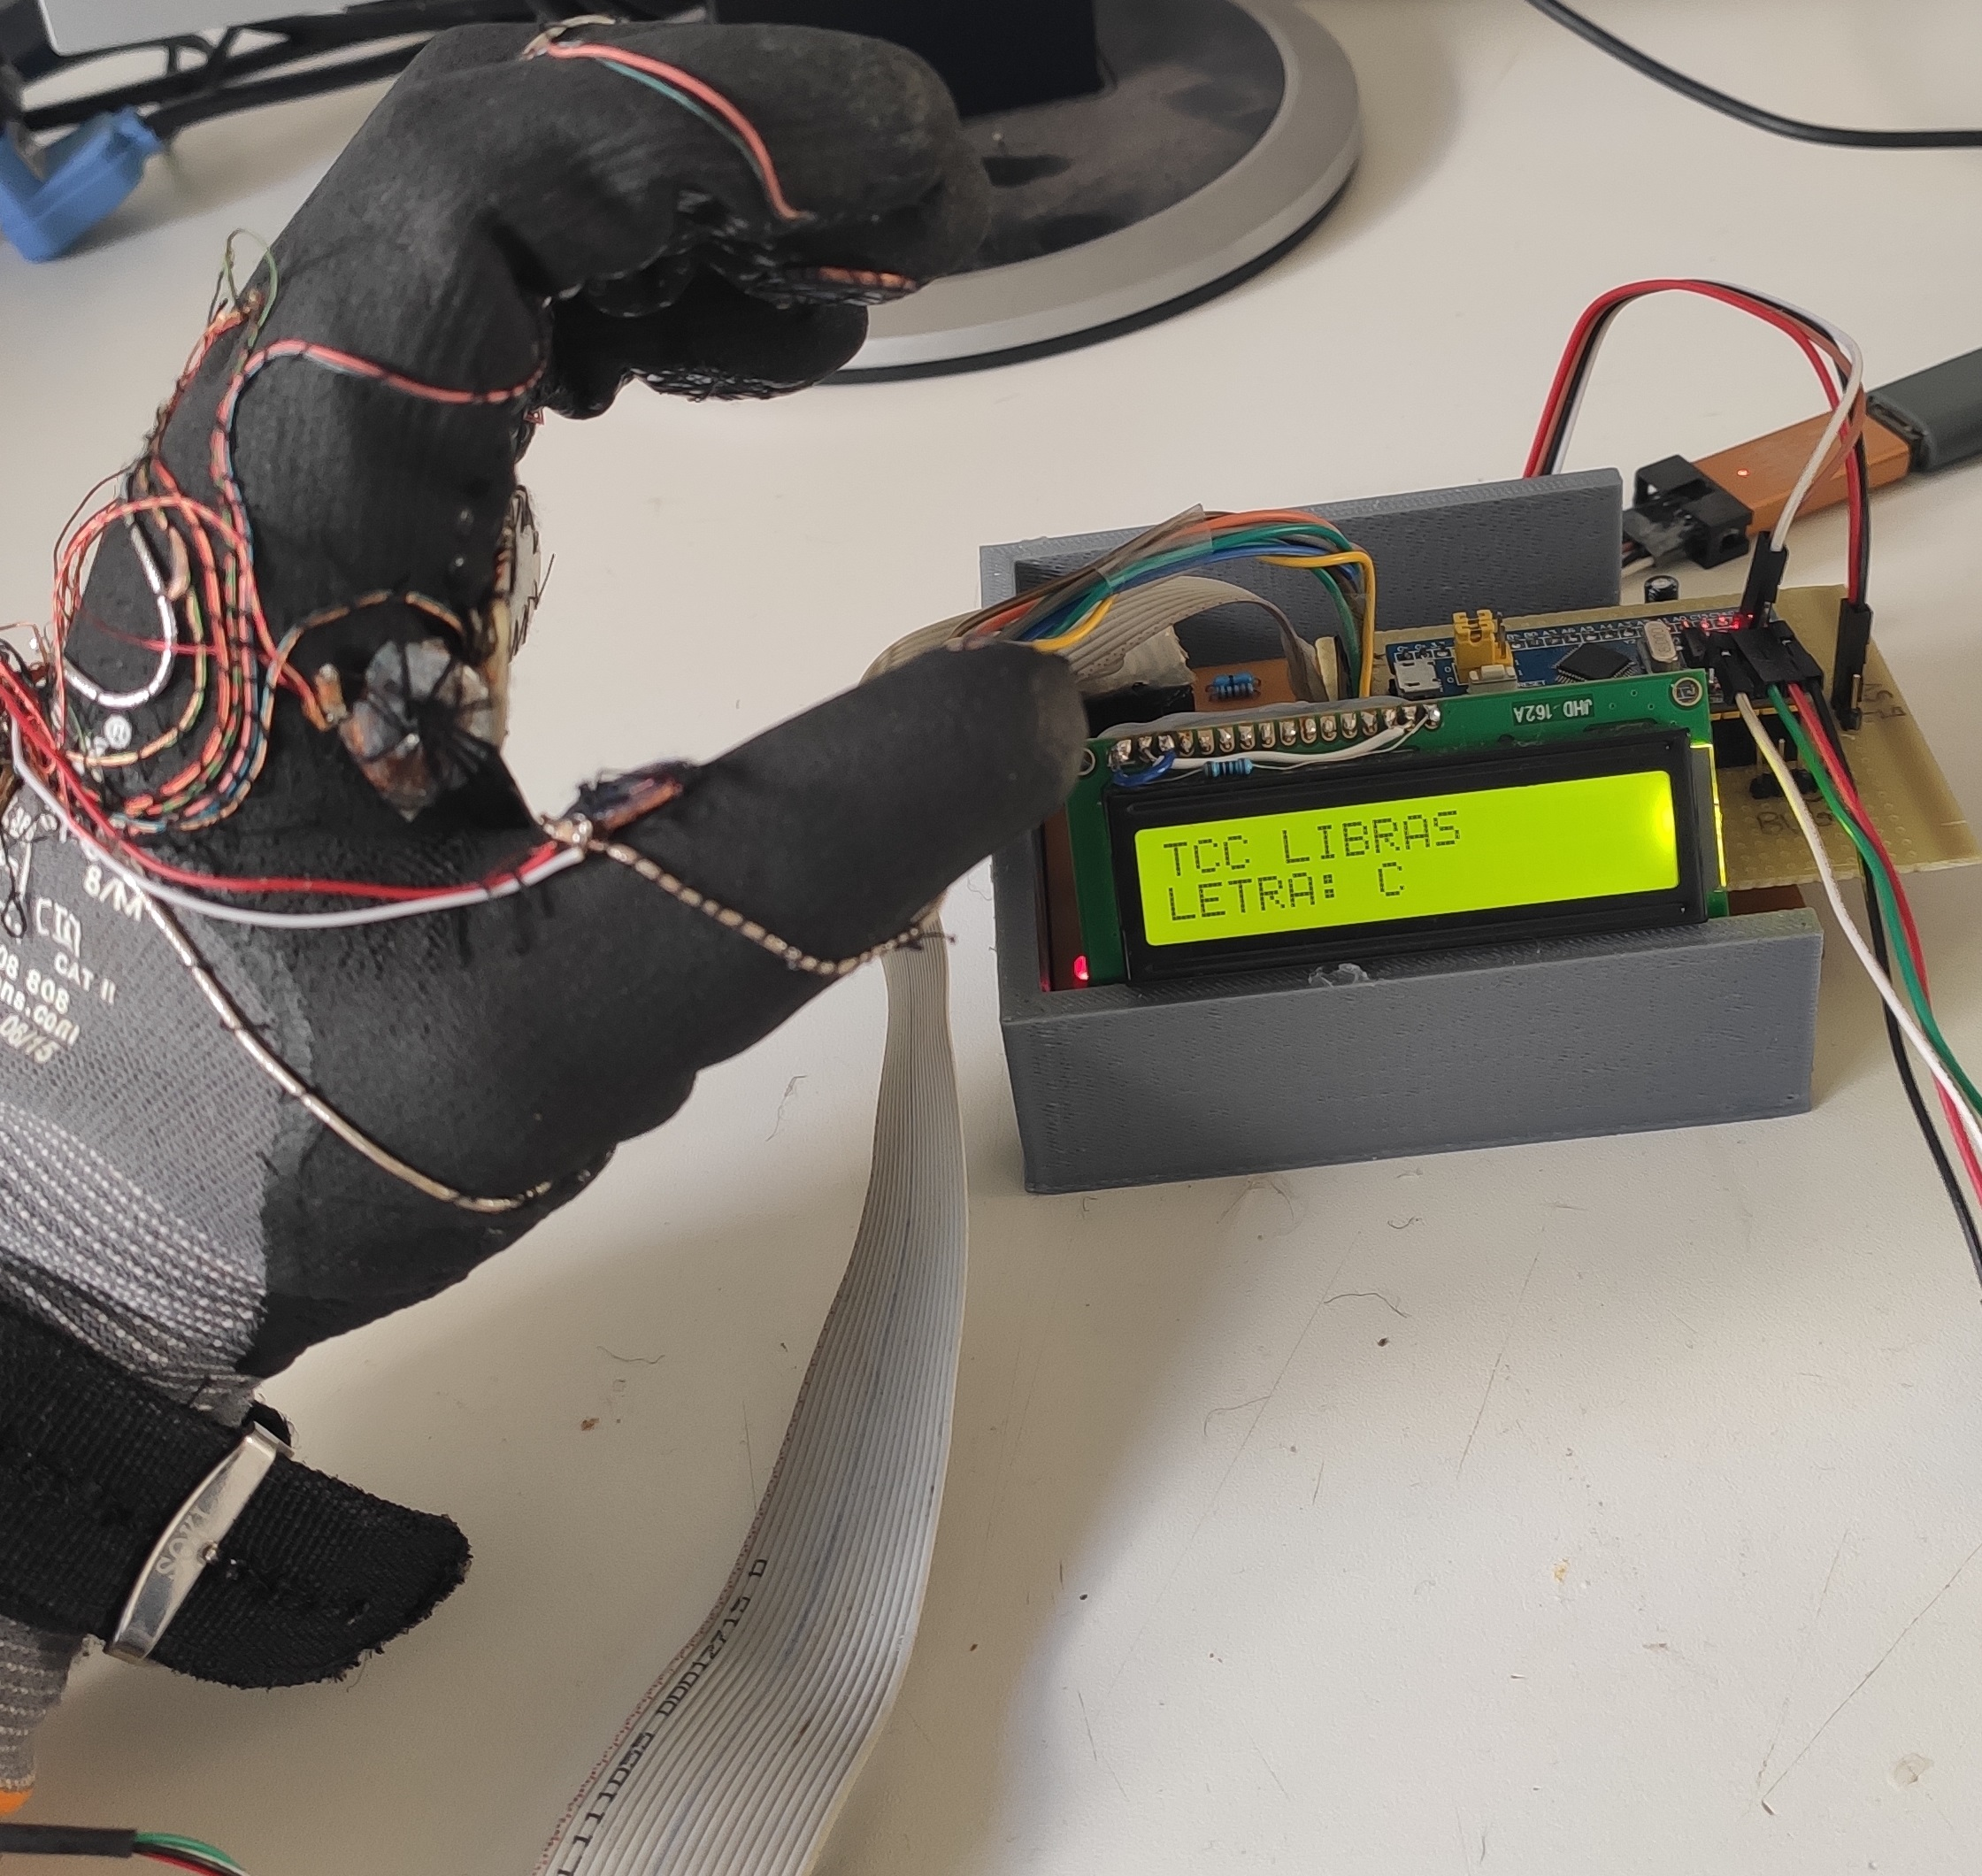
\includegraphics[scale=0.15]{imagens/LetraCLuva.jpg}
	\caption{Demonstração da letra C.}
	\label{fig:letraC}
\end{figure}



 Esse grupo de letras já era classificado no trabalho anterior, mas como a rede foi refeita, ela deve ser validada. Na Tabela \ref{tab:confusaosemconf}, está a matriz de confusão dessa rede refeita, onde foram testada cada letra dez vezes em sequência aleatória.

\begin{table}[H]
	\centering
	\resizebox{\textwidth}{!}{%
		\begin{tabular}{cl|l|l|l|l|l|l|l|l|l|l|l|l|l|l|l|l|l|l|l|}
			\cline{3-21}
			\multicolumn{1}{l}{} &  & \multicolumn{19}{c|}{Classe Predita} \\ \cline{3-21} 
			\multicolumn{1}{l}{} & \textbf{} & \textbf{A} & \textbf{B} & \textbf{C} & \textbf{D} & \textbf{E} & \textbf{F} & \textbf{G} & \textbf{L} & \textbf{M} & \textbf{N} & \textbf{O} & \textbf{Q} & \textbf{R} & \textbf{S} & \textbf{T} & \textbf{U} & \textbf{V} & \textbf{W} & \textbf{Y} \\ \hline
			\multicolumn{1}{|c|}{\multirow{19}{*}{\begin{tabular}[c]{@{}c@{}}C\\ l\\ a\\ s\\ s\\ e\\ \\ R\\ e\\ a\\ l\end{tabular}}} & \textbf{A} & 15 &  &  &  &  &  &  &  &  &  &  &  &  &  &  &  &  &  &  \\ \cline{2-21} 
			\multicolumn{1}{|c|}{} & \textbf{B} &  & 13 & 2 &  &  &  &  &  &  &  &  &  &  &  &  &  &  & \multicolumn{1}{c|}{} &  \\ \cline{2-21} 
			\multicolumn{1}{|c|}{} & \textbf{C} &  &  & 15 &  &  &  &  &  &  &  &  &  &  &  &  &  &  &  &  \\ \cline{2-21} 
			\multicolumn{1}{|c|}{} & \textbf{D} &  &  & 2 & 13 &  &  &  &  &  &  &  &  &  &  &  &  &  &  &  \\ \cline{2-21} 
			\multicolumn{1}{|c|}{} & \textbf{E} &  &  &  &  & 12 &  &  &  &  &  &  &  &  & 3 &  &  &  &  &  \\ \cline{2-21} 
			\multicolumn{1}{|c|}{} & \textbf{F} &  &  &  &  &  & 15 &  &  &  &  &  &  &  &  &  &  &  &  &  \\ \cline{2-21} 
			\multicolumn{1}{|c|}{} & \textbf{G} &  &  &  &  &  &  & 14 & 1 &  &  &  &  &  &  &  &  &  &  &  \\ \cline{2-21} 
			\multicolumn{1}{|c|}{} & \textbf{L} &  &  &  &  &  &  &  & 13 &  &  &  &  &  & 2 &  &  &  &  &  \\ \cline{2-21} 
			\multicolumn{1}{|c|}{} & \textbf{M} &  & 2 &  &  &  &  &  &  & 13 &  &  &  &  &  &  &  &  &  &  \\ \cline{2-21} 
			\multicolumn{1}{|c|}{} & \textbf{N} &  &  &  &  &  &  &  &  &  & 15 &  &  &  &  &  &  &  &  &  \\ \cline{2-21} 
			\multicolumn{1}{|c|}{} & \textbf{O} &  &  &  &  &  &  &  &  &  &  & 15 &  &  &  &  &  &  &  &  \\ \cline{2-21} 
			\multicolumn{1}{|c|}{} & \textbf{Q} &  &  &  &  &  &  &  &  &  &  &  & 13 &  & 2 &  &  &  &  &  \\ \cline{2-21} 
			\multicolumn{1}{|c|}{} & \textbf{R} &  &  &  &  &  &  &  &  &  &  &  &  & 15 &  &  &  &  &  &  \\ \cline{2-21} 
			\multicolumn{1}{|c|}{} & \textbf{S} &  &  &  &  &  &  &  &  &  &  &  &  &  & 15 &  &  &  &  &  \\ \cline{2-21} 
			\multicolumn{1}{|c|}{} & \textbf{T} &  &  &  &  &  &  &  &  &  &  &  &  &  &  & 15 &  &  &  &  \\ \cline{2-21} 
			\multicolumn{1}{|c|}{} & \textbf{U} &  &  &  &  &  &  &  &  &  &  &  &  & 3 &  &  & 12 &  &  &  \\ \cline{2-21} 
			\multicolumn{1}{|c|}{} & \textbf{V} &  &  &  &  &  &  &  &  &  &  &  &  &  &  &  & 1 & 14 &  &  \\ \cline{2-21} 
			\multicolumn{1}{|c|}{} & \textbf{W} &  &  &  &  &  &  &  &  &  &  &  &  &  &  &  &  & 2 & 13 &  \\ \cline{2-21} 
			\multicolumn{1}{|c|}{} & \textbf{Y} & 1 &  &  &  &  &  &  &  &  &  &  &  &  &  &  &  &  &  & 14 \\ \hline
		\end{tabular}%
	}
	\caption{Matriz de confusão das letras sem conflito}
	\label{tab:confusaosemconf}
\end{table}

Contanto todos os erros obtidos da Tabela \ref{tab:confusaosemconf}, temos um total de 21 vezes que uma classe foi classificadas erroneamente. Obtendo um total de 92,63\% de acerto, muito próximo dos 96,36\% de resultado do treinamento.


Agora para as letras conflitantes, como já explicado, a rede neural feita para classificar os movimentos obteve os resultados demonstrados pela Tabela \ref{tab:confusaoconf}.
\begin{table}[H]
	\centering
	\begin{tabular}{cc|c|c|c|c|c|c|c|}
		\cline{3-9}
		&  & \multicolumn{7}{c|}{Classe Predita} \\ \cline{3-9} 
		& \textbf{} & \textbf{I} & \textbf{J} & \textbf{K} & \textbf{H} & \textbf{P} & \textbf{Z} & \textbf{X} \\ \hline
		\multicolumn{1}{|c|}{\multirow{7}{*}{\begin{tabular}[c]{@{}c@{}}R\\ e\\ a\\ l\end{tabular}}} & \textbf{I} & 15 &  &  &  &  &  &  \\ \cline{2-9} 
		\multicolumn{1}{|c|}{} & \textbf{J} & 3 & 10 & 2 &  &  &  &  \\ \cline{2-9} 
		\multicolumn{1}{|c|}{} & \textbf{K} &  &  & 12 &  & 3 &  &  \\ \cline{2-9} 
		\multicolumn{1}{|c|}{} & \textbf{H} &  &  &  & 13 & 2 &  &  \\ \cline{2-9} 
		\multicolumn{1}{|c|}{} & \textbf{P} &  &  &  &  & 15 &  &  \\ \cline{2-9} 
		\multicolumn{1}{|c|}{} & \textbf{Z} &  &  &  &  &  & 15 &  \\ \cline{2-9} 
		\multicolumn{1}{|c|}{} & \textbf{X} &  &  &  &  &  & 6 & 9 \\ \hline
	\end{tabular}
	\caption{Matriz de confusão das letras conflitantes}
	\label{tab:confusaoconf}
\end{table}

Considerando a matriz das letras conflitantes da Tabela \ref{tab:confusaoconf}, temos 88,7\% de acerto, um percentual bom comparado aos 100\% aos do resultado do treinamento no código em Python.

Reunindo o resultado das duas redes, tem-se um percentual de 88,7\% de acerto. Esses 11,3 \% de erro são justificados por vários fatores. Um deles são os pontos cegos dos sensores indutivos como \citeonline{RUANI} descreve nos em seus resultados que podem ser resolvidos modificando a posição dos sensores e adicionando mais sensores indutivos. Também se deve ao fato de se estar utilizando somente o acelerômetro na classificação, onde poderia obter maior precisão utilizando giroscópio. A abordagem de janela deslizante funcionou bem, mas para uma classificação mais efetiva seria necessário uma abordagem de um algoritmo de aprendizagem de máquina que considera o tempo para aumentar essa taxa de acerto.

\chapter{Conclusões}

	O presente trabalho resultou em aprimoramento em um sistema de reconhecimento de letras do alfabeto de LIBRAS, permitindo detectar letras que contém movimento e completando as letras identificáveis pelo sistema. O código foi portado, obviamente com alterações para funcionar corretamente e a coleta dos dados do sensor inercial e as redes neurais funcionaram. A única coisa que não foi possível cumprir foi o teste com outros usuários para validar o funcionamento do sistema.


    A luva, a qual já havia sido construída em um trabalho anterior, possui fios e sensores expostos e frágeis. Então o manuseio da luva teve que ser bem delicado pois os fios das bobinas sempre soltavam, necessitando reparos. Uma solução pra isso em um trabalho futuro seria trocar a luva e esconder a fiação. Também escolher uma luva mais flexível, pois em alguns sinais é necessário fazer um pouco de força para a sinalização correta da letra, o que também pode vir a danificar os sensores. A comunicação I2C utilizada com o sensor inercial se mostrou pouco robusta por causa do tamanho do cabo (inicialmente 60 cm), que teve que ser reduzido para não causar tantos problemas de comunicação.
    
    Com relação ao microcontrolador, este foi suficiente para a demanda de processamento. Apesar disso, devido a abordagem de \textit{software} com \textit{background/foreground}, foi necessário temporizar e diminuir a frequência que se capturava os sinais. Como a aplicação é sensível ao tempo, seria interessante aplicar um \textit{protothread} ou um sistema operacional de tempo real para eliminar algumas esperas ocupadas.
    
    Para trabalhos futuros, como identificar sinais de LIBRAS simbolizam palavras e utilizam apenas uma mão e sem expressões faciais, seria necessário uma analise sobre o sensor inercial, trocando algumas posições de sensores para as características da rede neural ficarem mais marcantes. Para o processamento dos dados do sensor inercial poderia ser estudado e implementado o código que o microcontrolador do sensor já realiza os cálculos dos ângulos de rotação(\textit{Pitch, Yaw}) e se aplicar um sensor inercial de 9 ou 10 graus de liberdade para melhorar a precisão dos sinais lidos do sensor inercial.

    Caso seja a intenção de implementar sinais com duas mãos, seria necessário outra luva, mas a demanda de tempo para a leitura das duas poderia ser elevada. Por isso deve-se utilizar a abordagem da luva com mais tipos de sensores, por exemplo alguns sensores resistivos de flexão, que são lidos mais rapidamente e simples de interpretar, juntamente com sensores inerciais de 9 ou 10 graus de liberdade.
    
    E  por fim, para implementar um sistema completo para identificar sinais e expressões faciais, seria necessário implementar processamento de imagem.
    

\sigla{12}{asdasdas}


\apendice
\chapter{Códigos desenvolvidos}
	Os códigos desenvolvidos neste trabalho estão disponíveis em \citeonline{gitmeu}.
	
	O Código \ref{cod:start} inicia os periféricos utilizados neste trabalho, também inicia o sensor inercial e o \textit{display}. Ao iniciar, são necessários 10 segundos de espera para o funcionamento correto, essa espera é exibido no \textit{display}. Após a espera, é iniciado o sensor inercial e o código entra no laço principal.
\begin{figure}[H]
	\begin{lstlisting}[breaklines, style=CStyle, , frame=single, caption=Rotina de inicialização do projeto,  label=cod:start]
void StartProjeto(void) {
	ind_set_tim(&htim1);
	ind_set_adc(&hadc1);
	i2c_init(&hi2c1);
	tim4_init(&htim4);
	uart_init(&huart3);
	uart_receive_it(&uart_d, 1);
	lcd16x2_init(LCD16X2_DISPLAY_ON_CURSOR_OFF_BLINK_OFF);
	lcd16x2_puts("Iniciando Sensor MPU");
	for(uint8_t i = 0; i < 10; i++) {
		HAL_Delay(1000);
		lcd16x2_clrscr();
		lcd16x2_puts("Iniciando em ");
		lcd16x2_gotoxy(0, 1);
		lcd16x2_putc(i + 49);
	}	
	lcd16x2_putc(result);
	if(!i2c_device_ready(MPU_ADDR)) {
		asm("NOP");
		while(1);
	}	
	mpu_init(&mpu);
	mpu.acc_res = ACC_SENS_2;
	mpu_set_offset_acc_x(ACC_OFF_X);
	mpu_set_offset_acc_y(ACC_OFF_Y);
	mpu_set_offset_acc_z(ACC_OFF_Z);
	lcd16x2_clrscr();
	lcd16x2_gotoxy(0, 0);
	lcd16x2_puts("TCC LIBRAS\nLETRA: -");
}
	\end{lstlisting}
	\caption*{Fonte: Autoria própria.}
\end{figure}
	
	O Código \ref{cod:Indutivo} faz a coleta dos sensores indutivos, selecionando um dos 12 pares de sensor/gerador e ativando o \textit{clock}. Após 4 $ms$ é feita a leitura do conversor A/D (Analógico para Digital). O valor desta leitura é armazenado em um vetor.
\begin{figure}[H]
\begin{lstlisting}[style=CStyle, breaklines, frame=single, caption=Rotina de coleta de dados do sensor indutivo,  label=cod:Indutivo]
void feedTheInductiveSensor(void) {
	for(uint8_t i = 0; i < 12; i++) {
		ind_set_ger(ger[i]);
		ind_set_sen(sen[i]);
		ind_set_pwm(pwm[i]);
		HAL_Delay(5);
		ind_start_conversion();
		while(!ind_get_conv_finish());
		valores[i] = ind_get_conv_value();
	}
}
\end{lstlisting}
\caption*{Fonte: Autoria própria.}
\end{figure}

No Código \ref{cod:mainloop}, é demonstrado o laço principal do programa. Antes de entrar no laço, são iniciados os periféricos e variáveis na função \textit{StartProjeto},  e repete-se a captura dos dados do sensor indutivo e realiza-se a classificação. Uma interface serial foi configurada para a transferência dos dados do microcontrolador para o computador para treinamento de rede neural. E quando um dado chega na interface serial, a função \textit{sendToSerial} é chamada para mandar os dados dos sensores.

\begin{figure}[H]
\begin{lstlisting}[style=CStyle, breaklines, frame=single, caption=Laço principal do \textit{firmware},  label=cod:mainloop]
int main(void) 
{
	StartProjeto();
	while (1)
	{
		feedTheInductiveSensor();
		if(xSemSerial) {
			sendToSerial();
		}
		classifyLetter();
	}
}
\end{lstlisting}
\caption*{Fonte: Autoria própria.}
\end{figure}

O Código \ref{cod:rede1} é o treinamento da rede neural para os sensores indutivos em Python, onde é utilizado 75\% dos dados para treinamento e 25\% dos dados para teste.
\begin{figure}[H]
\begin{lstlisting}[breaklines, frame=single, caption=Treinamento da rede neural dos sensores indutivos em Python, style=CStyle, label=cod:rede1]
def treinamento(activation, hidden_layers, verbose=False):
	caracteristicas = arruma_dados()
	scaler = pre.MinMaxScaler(feature_range=(-1,1))
	scaler.fit(caracteristicas)
	caracteristicas = scaler.transform(caracteristicas)
	
	x_train, x_test, y_train, y_test = train_test_split(caracteristicas, classes, test_size=0.25)
	clf = MLPClassifier(hidden_layer_sizes=(hidden_layers,), activation=activation, max_iter=1500, shuffle=True, n_iter_no_change=100)
	
	clf.fit(x_train, y_train)
	y_pred = clf.predict(x_test)
	
	return clf
\end{lstlisting}
\caption*{Fonte: Autoria própria.}
\end{figure}

Para a implementação do código da rede treinando no microcontrolador, o Código \ref{cod:defines1} exibe a quantia de entradas, o número de camadas ocultas e o número de saídas da rede. Também são exibidos todos os pesos e os \textit{bias} da rede treinada.

\begin{figure}[H]
	\begin{lstlisting}[breaklines, frame=single, caption=Definições da rede neural dos sensores indutivos, style=CStyle, label=cod:defines1]
#define NUMBER_OF_INPUTS               12
#define NUMBER_OF_HIDDEN               21
#define NUMBER_OF_OUTPUTS              22
float weightInputHidden[NUMBER_OF_INPUTS][NUMBER_OF_HIDDEN] {...};
float weightHiddenOutput[NUMBER_OF_HIDDEN][NUMBER_OF_OUTPUTS] = {...};
float biasHidden[NUMBER_OF_HIDDEN] = {...};
float biasOutput[NUMBER_OF_OUTPUTS] = {...};
	\end{lstlisting}
	\caption*{Fonte: Autoria própria.}
\end{figure}
	
	No Código \ref{cod:feedforward1}, é apresentada a rotina de \textit{feedforward} dos sensores indutivos, os valores dos sensores são a entrada, e baseado nos pesos treinados da rede neural, é dado um resultado da classificação.
	
\begin{figure}[H]
\begin{lstlisting}[breaklines, frame=single, caption=\textit{Feedforward implementado no microcontrolador}, style=CStyle, label=cod:feedforward1]
void classSystemPredict(float * entrada, float * saida) {
	float oculta[NUMBER_OF_HIDDEN];
	float sum = 0;
	
	for(int i = 0; i < NUMBER_OF_HIDDEN; i++) {
		sum = 0;
		for(int ii = 0; ii < NUMBER_OF_INPUTS; ii++) {
		sum += entrada[ii] * weightInputHidden[ii][i];
		}
		oculta[i] = tanhf(sum + biasHidden[i]);
	}
	
	for(int i = 0; i < NUMBER_OF_OUTPUTS; i++) {
		float sum = 0;
		for(int ii = 0; ii < NUMBER_OF_HIDDEN; ii++) {
		sum += oculta[ii] * weightHiddenOutput[ii][i];
		}
		saida[i] = tanhf(sum + biasOutput[i]);
	}
}
\end{lstlisting}
\caption*{Fonte: Autoria própria.}
\end{figure}
	
	\begin{figure}[H]
	
	O pós-processamento da rede neural dos sensores indutivos é feito verificando qual foi a saída com o maior valor, variando de 0 a 0,99. A classe com o maior valor é a saída da rede. 
\begin{lstlisting}[breaklines, frame=single, caption=Pós processamento da rede neural dos sensores indutivos, style=CStyle, label=cod:pos1]
char classSystemPostProcess(float * saidas) {
	float max = 0;
	int ind = 0;
	for (int i = 0; i < NUMBER_OF_OUTPUTS; i++) {
		if(max < saidas[i]) {
			max = saidas[i];
			ind = i;
		}
	}
	char ret[] = {'A', 'B', 'C', 'D', 'E','F', 'G', '1', '2', 'L', 'M', 'N', 'O', 'Q', 'R', 'S', 'T', 'U', 'V', 'W', 'Y', '3'};
	return ret[ind];
}
\end{lstlisting}
\caption*{Fonte: Autoria própria.}
\end{figure}

O Código \ref{cod:rede2} é o treinamento da rede neural para o sensor inercial em Python, onde é utilizado 80\% dos dados para treinamento e 20\% dos dados para teste.
\begin{figure}[H]
\begin{lstlisting}[breaklines, frame=single, caption=Treinamento da rede neural do sensor inercial Python, style=CStyle, label=cod:rede2]
def TrainNeuralNet(data, classes, numberOfHidden, activationFunction, verbose=False):

	xData, yData = LoadDataFromCsv()
	scalledData, dataMin, dataMax = ScaleData(xData)
	xTrain, xTest, yTrain, yTest = train_test_split(data, classes, test_size=0.2)
	MLP = MLPClassifier(hidden_layer_sizes=(numberOfHidden,), activation=activationFunction, max_iter=10000, shuffle=True, n_iter_no_change=1000)
	MLP.fit(xTrain, yTrain)
	
	yPredict = MLP.predict(xTest)
\end{lstlisting}
\caption*{Fonte: Autoria própria.}
\end{figure}

Para a implementação da rede neural para o sensor inercial também são feitas as definições de quantidade de entrada, saída e número de camadas ocultas. O Código \ref{cod:defines2} demonstra essas definições e também os vetores com os pesos da rede já treinada.

\begin{figure}[H]
	\begin{lstlisting}[breaklines, frame=single, caption=Definições da rede neural dos sensores indutivos, style=CStyle, label=cod:defines2]
#define NUMBER_OF_INPUTS_A               40
#define NUMBER_OF_HIDDEN_A               40
#define NUMBER_OF_OUTPUTS_A              5

float weightInputHiddenA[NUMBER_OF_INPUTS_A][NUMBER_OF_HIDDEN_A] {...};
float weightHiddenOutputA[NUMBER_OF_HIDDEN_A][NUMBER_OF_OUTPUTS_A] = {...};
float biasHiddenA[NUMBER_OF_HIDDEN_A] = {...};
float biasOutputA[NUMBER_OF_OUTPUTS_A] = {...};
	\end{lstlisting}
	\caption*{Fonte: Autoria própria.}
\end{figure}

\begin{figure}[H]
\begin{lstlisting}[breaklines, frame=single, caption=Vetor de respostas possíveis do pós processamento da rede neural do sensor inercial, style=CStyle, label=cod:feedfor2]
char ret[] = {'-', 'K', 'J', 'H', 'X'};
\end{lstlisting}
\caption*{Fonte: Autoria própria.}
\end{figure}

 O Código \ref{cod:classify}, exibe a rotina de classificação. Após fazer a leitura dos sensores inerciais, é feita a classificação da letra, caso ela se encaixe nas classes 1, 2, ou 3, é acionada a captura dos dados do sensor inercial e feita a classificação do movimento. Finalmente o resultado é exibido no \textit{display}.
\begin{figure}[H]
\begin{lstlisting}[breaklines, frame=single, caption=Função que executa a classificação das letras, style=CStyle, label=cod:classify]
void classifyLetter(void) {
	lcd16x2_gotoxy(7, 1);
	float input[NUMBER_OF_INPUTS];
	float outpu[NUMBER_OF_OUTPUTS];
	for(uint8_t i = 0; i < NUMBER_OF_INPUTS; i++)
		input[i] = (float)valores[i];
		
	classSystemScaleDataInput(input);
	classSystemPredict(input, outpu);
	result = classSystemPostProcess(outpu);
	HAL_Delay(50);
	if(result == '1' || result == '2' || result == '3') {
		getMpuValues();
		classifyMoviment(result);
	} else {
		lcd16x2_gotoxy(7, 1);
		lcd16x2_putc(result);
	}
}
\end{lstlisting}
\caption*{Fonte: Autoria própria.}
\end{figure}
\bibliographystyle{abnt-alf} 
\bibliography{Refs/Ref}
  
\end{document}

